\documentclass[twoside]{book}

% Packages required by doxygen
\usepackage{fixltx2e}
\usepackage{calc}
\usepackage{doxygen}
\usepackage[export]{adjustbox} % also loads graphicx
\usepackage{graphicx}
\usepackage[utf8]{inputenc}
\usepackage{makeidx}
\usepackage{multicol}
\usepackage{multirow}
\PassOptionsToPackage{warn}{textcomp}
\usepackage{textcomp}
\usepackage[nointegrals]{wasysym}
\usepackage[table]{xcolor}

% Font selection
\usepackage[T1]{fontenc}
\usepackage[scaled=.90]{helvet}
\usepackage{courier}
\usepackage{amssymb}
\usepackage{sectsty}
\renewcommand{\familydefault}{\sfdefault}
\allsectionsfont{%
  \fontseries{bc}\selectfont%
  \color{darkgray}%
}
\renewcommand{\DoxyLabelFont}{%
  \fontseries{bc}\selectfont%
  \color{darkgray}%
}
\newcommand{\+}{\discretionary{\mbox{\scriptsize$\hookleftarrow$}}{}{}}

% Page & text layout
\usepackage{geometry}
\geometry{%
  a4paper,%
  top=2.5cm,%
  bottom=2.5cm,%
  left=2.5cm,%
  right=2.5cm%
}
\tolerance=750
\hfuzz=15pt
\hbadness=750
\setlength{\emergencystretch}{15pt}
\setlength{\parindent}{0cm}
\setlength{\parskip}{3ex plus 2ex minus 2ex}
\makeatletter
\renewcommand{\paragraph}{%
  \@startsection{paragraph}{4}{0ex}{-1.0ex}{1.0ex}{%
    \normalfont\normalsize\bfseries\SS@parafont%
  }%
}
\renewcommand{\subparagraph}{%
  \@startsection{subparagraph}{5}{0ex}{-1.0ex}{1.0ex}{%
    \normalfont\normalsize\bfseries\SS@subparafont%
  }%
}
\makeatother

% Headers & footers
\usepackage{fancyhdr}
\pagestyle{fancyplain}
\fancyhead[LE]{\fancyplain{}{\bfseries\thepage}}
\fancyhead[CE]{\fancyplain{}{}}
\fancyhead[RE]{\fancyplain{}{\bfseries\leftmark}}
\fancyhead[LO]{\fancyplain{}{\bfseries\rightmark}}
\fancyhead[CO]{\fancyplain{}{}}
\fancyhead[RO]{\fancyplain{}{\bfseries\thepage}}
\fancyfoot[LE]{\fancyplain{}{}}
\fancyfoot[CE]{\fancyplain{}{}}
\fancyfoot[RE]{\fancyplain{}{\bfseries\scriptsize Generated by Doxygen }}
\fancyfoot[LO]{\fancyplain{}{\bfseries\scriptsize Generated by Doxygen }}
\fancyfoot[CO]{\fancyplain{}{}}
\fancyfoot[RO]{\fancyplain{}{}}
\renewcommand{\footrulewidth}{0.4pt}
\renewcommand{\chaptermark}[1]{%
  \markboth{#1}{}%
}
\renewcommand{\sectionmark}[1]{%
  \markright{\thesection\ #1}%
}

% Indices & bibliography
\usepackage{natbib}
\usepackage[titles]{tocloft}
\setcounter{tocdepth}{3}
\setcounter{secnumdepth}{5}
\makeindex

% Hyperlinks (required, but should be loaded last)
\usepackage{ifpdf}
\ifpdf
  \usepackage[pdftex,pagebackref=true]{hyperref}
\else
  \usepackage[ps2pdf,pagebackref=true]{hyperref}
\fi
\hypersetup{%
  colorlinks=true,%
  linkcolor=blue,%
  citecolor=blue,%
  unicode%
}

% Custom commands
\newcommand{\clearemptydoublepage}{%
  \newpage{\pagestyle{empty}\cleardoublepage}%
}

\usepackage{caption}
\captionsetup{labelsep=space,justification=centering,font={bf},singlelinecheck=off,skip=4pt,position=top}

%===== C O N T E N T S =====

\begin{document}

% Titlepage & ToC
\hypersetup{pageanchor=false,
             bookmarksnumbered=true,
             pdfencoding=unicode
            }
\pagenumbering{alph}
\begin{titlepage}
\vspace*{7cm}
\begin{center}%
{\Large Vessel \\[1ex]\large 1.\+0 }\\
\vspace*{1cm}
{\large Generated by Doxygen 1.8.13}\\
\end{center}
\end{titlepage}
\clearemptydoublepage
\pagenumbering{roman}
\tableofcontents
\clearemptydoublepage
\pagenumbering{arabic}
\hypersetup{pageanchor=true}

%--- Begin generated contents ---
\chapter{Hierarchical Index}
\section{Class Hierarchy}
This inheritance list is sorted roughly, but not completely, alphabetically\+:\begin{DoxyCompactList}
\item \contentsline{section}{A\+PI}{\pageref{class_a_p_i}}{}
\begin{DoxyCompactList}
\item \contentsline{section}{Backup\+A\+PI}{\pageref{class_backup_a_p_i}}{}
\end{DoxyCompactList}
\item \contentsline{section}{Auth}{\pageref{class_auth}}{}
\item \contentsline{section}{Backup\+A\+P\+I\+Session}{\pageref{class_backup_a_p_i_session}}{}
\item \contentsline{section}{Backup\+Database}{\pageref{class_backup_database}}{}
\item \contentsline{section}{Backup\+:\+:File\+:\+:Backup\+File}{\pageref{class_backup_1_1_file_1_1_backup_file}}{}
\item \contentsline{section}{Backup\+File}{\pageref{class_backup_file}}{}
\item \contentsline{section}{Backup\+L\+D\+AP}{\pageref{class_backup_l_d_a_p}}{}
\item \contentsline{section}{Backup\+Log}{\pageref{class_backup_log}}{}
\item \contentsline{section}{Backup\+Machine}{\pageref{class_backup_machine}}{}
\item \contentsline{section}{Backup\+Session}{\pageref{class_backup_session}}{}
\item \contentsline{section}{Backup\+Upload}{\pageref{class_backup_upload}}{}
\item \contentsline{section}{Backup\+User}{\pageref{class_backup_user}}{}
\item \contentsline{section}{Backup\+:\+:Networking\+:\+:Client}{\pageref{class_backup_1_1_networking_1_1_client}}{}
\item \contentsline{section}{Backup\+:\+:Compression\+:\+:Compressor}{\pageref{class_backup_1_1_compression_1_1_compressor}}{}
\item enable\+\_\+shared\+\_\+from\+\_\+this\begin{DoxyCompactList}
\item \contentsline{section}{Backup\+:\+:Networking\+:\+:Connection}{\pageref{class_backup_1_1_networking_1_1_connection}}{}
\end{DoxyCompactList}
\item \contentsline{section}{Backup\+:\+:Types\+:\+:file\+\_\+data}{\pageref{struct_backup_1_1_types_1_1file__data}}{}
\item \contentsline{section}{Backup\+:\+:Types\+:\+:file\+\_\+directory}{\pageref{struct_backup_1_1_types_1_1file__directory}}{}
\item \contentsline{section}{Backup\+:\+:File\+:\+:File\+Iterator}{\pageref{class_backup_1_1_file_1_1_file_iterator}}{}
\item \contentsline{section}{Backup\+:\+:Types\+:\+:http\+\_\+request}{\pageref{struct_backup_1_1_types_1_1http__request}}{}
\item \contentsline{section}{Backup\+:\+:Types\+:\+:http\+\_\+upload\+\_\+file}{\pageref{struct_backup_1_1_types_1_1http__upload__file}}{}
\item \contentsline{section}{Backup\+:\+:Networking\+:\+:Http\+Request}{\pageref{class_backup_1_1_networking_1_1_http_request}}{}
\item \contentsline{section}{Backup\+:\+:Database\+:\+:Local\+Database}{\pageref{class_backup_1_1_database_1_1_local_database}}{}
\item \contentsline{section}{Backup\+:\+:Logging\+:\+:Log}{\pageref{class_backup_1_1_logging_1_1_log}}{}
\item \contentsline{section}{Backup\+:\+:Networking\+:\+:Server}{\pageref{class_backup_1_1_networking_1_1_server}}{}
\item \contentsline{section}{Backup\+:\+:Compression\+:\+:Tarball}{\pageref{class_backup_1_1_compression_1_1_tarball}}{}
\end{DoxyCompactList}

\chapter{Class Index}
\section{Class List}
Here are the classes, structs, unions and interfaces with brief descriptions\+:\begin{DoxyCompactList}
\item\contentsline{section}{\hyperlink{class_a_p_i}{A\+PI} }{\pageref{class_a_p_i}}{}
\item\contentsline{section}{\hyperlink{class_auth}{Auth} }{\pageref{class_auth}}{}
\item\contentsline{section}{\hyperlink{class_backup_a_p_i}{Backup\+A\+PI} }{\pageref{class_backup_a_p_i}}{}
\item\contentsline{section}{\hyperlink{class_backup_a_p_i_session}{Backup\+A\+P\+I\+Session} }{\pageref{class_backup_a_p_i_session}}{}
\item\contentsline{section}{\hyperlink{class_backup_database}{Backup\+Database} }{\pageref{class_backup_database}}{}
\item\contentsline{section}{\hyperlink{class_backup_1_1_file_1_1_backup_file}{Backup\+::\+File\+::\+Backup\+File} }{\pageref{class_backup_1_1_file_1_1_backup_file}}{}
\item\contentsline{section}{\hyperlink{class_backup_file}{Backup\+File} }{\pageref{class_backup_file}}{}
\item\contentsline{section}{\hyperlink{class_backup_l_d_a_p}{Backup\+L\+D\+AP} }{\pageref{class_backup_l_d_a_p}}{}
\item\contentsline{section}{\hyperlink{class_backup_log}{Backup\+Log} }{\pageref{class_backup_log}}{}
\item\contentsline{section}{\hyperlink{class_backup_machine}{Backup\+Machine} }{\pageref{class_backup_machine}}{}
\item\contentsline{section}{\hyperlink{class_backup_session}{Backup\+Session} }{\pageref{class_backup_session}}{}
\item\contentsline{section}{\hyperlink{class_backup_upload}{Backup\+Upload} }{\pageref{class_backup_upload}}{}
\item\contentsline{section}{\hyperlink{class_backup_user}{Backup\+User} }{\pageref{class_backup_user}}{}
\item\contentsline{section}{\hyperlink{class_backup_1_1_networking_1_1_client}{Backup\+::\+Networking\+::\+Client} }{\pageref{class_backup_1_1_networking_1_1_client}}{}
\item\contentsline{section}{\hyperlink{class_backup_1_1_compression_1_1_compressor}{Backup\+::\+Compression\+::\+Compressor} }{\pageref{class_backup_1_1_compression_1_1_compressor}}{}
\item\contentsline{section}{\hyperlink{class_backup_1_1_networking_1_1_connection}{Backup\+::\+Networking\+::\+Connection} }{\pageref{class_backup_1_1_networking_1_1_connection}}{}
\item\contentsline{section}{\hyperlink{struct_backup_1_1_types_1_1file__data}{Backup\+::\+Types\+::file\+\_\+data} }{\pageref{struct_backup_1_1_types_1_1file__data}}{}
\item\contentsline{section}{\hyperlink{struct_backup_1_1_types_1_1file__directory}{Backup\+::\+Types\+::file\+\_\+directory} }{\pageref{struct_backup_1_1_types_1_1file__directory}}{}
\item\contentsline{section}{\hyperlink{class_backup_1_1_file_1_1_file_iterator}{Backup\+::\+File\+::\+File\+Iterator} }{\pageref{class_backup_1_1_file_1_1_file_iterator}}{}
\item\contentsline{section}{\hyperlink{struct_backup_1_1_types_1_1http__request}{Backup\+::\+Types\+::http\+\_\+request} }{\pageref{struct_backup_1_1_types_1_1http__request}}{}
\item\contentsline{section}{\hyperlink{struct_backup_1_1_types_1_1http__upload__file}{Backup\+::\+Types\+::http\+\_\+upload\+\_\+file} }{\pageref{struct_backup_1_1_types_1_1http__upload__file}}{}
\item\contentsline{section}{\hyperlink{class_backup_1_1_networking_1_1_http_request}{Backup\+::\+Networking\+::\+Http\+Request} }{\pageref{class_backup_1_1_networking_1_1_http_request}}{}
\item\contentsline{section}{\hyperlink{class_backup_1_1_database_1_1_local_database}{Backup\+::\+Database\+::\+Local\+Database} }{\pageref{class_backup_1_1_database_1_1_local_database}}{}
\item\contentsline{section}{\hyperlink{class_backup_1_1_logging_1_1_log}{Backup\+::\+Logging\+::\+Log} }{\pageref{class_backup_1_1_logging_1_1_log}}{}
\item\contentsline{section}{\hyperlink{class_backup_1_1_networking_1_1_server}{Backup\+::\+Networking\+::\+Server} }{\pageref{class_backup_1_1_networking_1_1_server}}{}
\item\contentsline{section}{\hyperlink{class_backup_1_1_compression_1_1_tarball}{Backup\+::\+Compression\+::\+Tarball} }{\pageref{class_backup_1_1_compression_1_1_tarball}}{}
\end{DoxyCompactList}

\chapter{Class Documentation}
\hypertarget{class_vessel_1_1_exception_1_1_aws_exception}{}\section{Vessel\+:\+:Exception\+:\+:Aws\+Exception Class Reference}
\label{class_vessel_1_1_exception_1_1_aws_exception}\index{Vessel\+::\+Exception\+::\+Aws\+Exception@{Vessel\+::\+Exception\+::\+Aws\+Exception}}
Inheritance diagram for Vessel\+:\+:Exception\+:\+:Aws\+Exception\+:\begin{figure}[H]
\begin{center}
\leavevmode
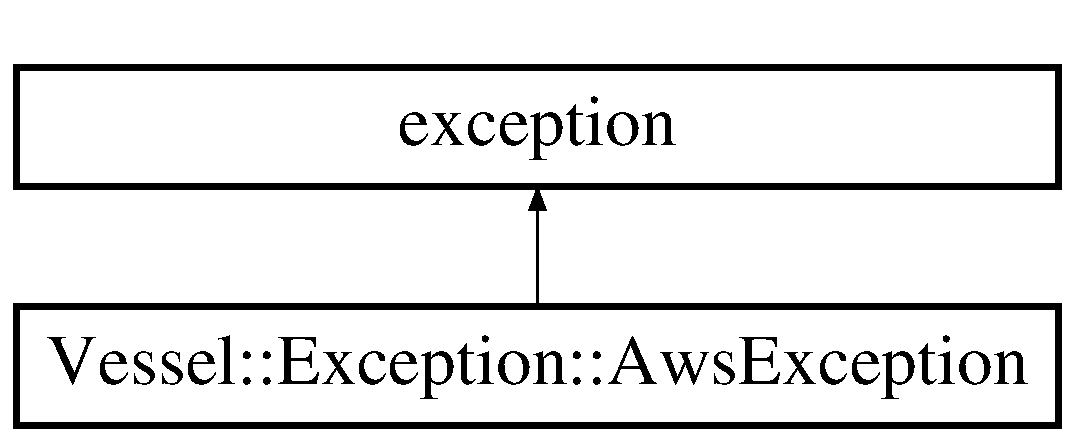
\includegraphics[height=2.000000cm]{class_vessel_1_1_exception_1_1_aws_exception}
\end{center}
\end{figure}
\subsection*{Public Types}
\begin{DoxyCompactItemize}
\item 
\mbox{\Hypertarget{class_vessel_1_1_exception_1_1_aws_exception_a37553d9ce96de364de06b14933d05a74}\label{class_vessel_1_1_exception_1_1_aws_exception_a37553d9ce96de364de06b14933d05a74}} 
enum {\bfseries Error\+Code} \{ \newline
{\bfseries No\+Error} = 0, 
{\bfseries Init\+Failed}, 
{\bfseries Upload\+Failed}, 
{\bfseries Bad\+Response}, 
\newline
{\bfseries Xml\+Parse\+Error}, 
{\bfseries Invalid\+Credentials}, 
{\bfseries Bad\+Signing\+Key}, 
{\bfseries Bad\+Upload\+Id}
 \}
\end{DoxyCompactItemize}
\subsection*{Public Member Functions}
\begin{DoxyCompactItemize}
\item 
\mbox{\Hypertarget{class_vessel_1_1_exception_1_1_aws_exception_a94f2924ba17eaac83338a0ffa5ae77d4}\label{class_vessel_1_1_exception_1_1_aws_exception_a94f2924ba17eaac83338a0ffa5ae77d4}} 
{\bfseries Aws\+Exception} (Error\+Code e, const std\+::string \&msg)
\item 
\mbox{\Hypertarget{class_vessel_1_1_exception_1_1_aws_exception_abe49e7827f65f817810f81d7179c6e56}\label{class_vessel_1_1_exception_1_1_aws_exception_abe49e7827f65f817810f81d7179c6e56}} 
Error\+Code {\bfseries get\+\_\+code} ()
\item 
\mbox{\Hypertarget{class_vessel_1_1_exception_1_1_aws_exception_a75571f88039a35f1b629247c88c0de1a}\label{class_vessel_1_1_exception_1_1_aws_exception_a75571f88039a35f1b629247c88c0de1a}} 
virtual const char $\ast$ {\bfseries what} () const noexcept override
\end{DoxyCompactItemize}


The documentation for this class was generated from the following file\+:\begin{DoxyCompactItemize}
\item 
/home/kyle/cpp/bv-\/backup/include/vessel/aws/aws\+\_\+exception.\+hpp\end{DoxyCompactItemize}

\hypertarget{class_vessel_1_1_networking_1_1_aws_s3_client}{}\section{Vessel\+:\+:Networking\+:\+:Aws\+S3\+Client Class Reference}
\label{class_vessel_1_1_networking_1_1_aws_s3_client}\index{Vessel\+::\+Networking\+::\+Aws\+S3\+Client@{Vessel\+::\+Networking\+::\+Aws\+S3\+Client}}
Inheritance diagram for Vessel\+:\+:Networking\+:\+:Aws\+S3\+Client\+:\begin{figure}[H]
\begin{center}
\leavevmode
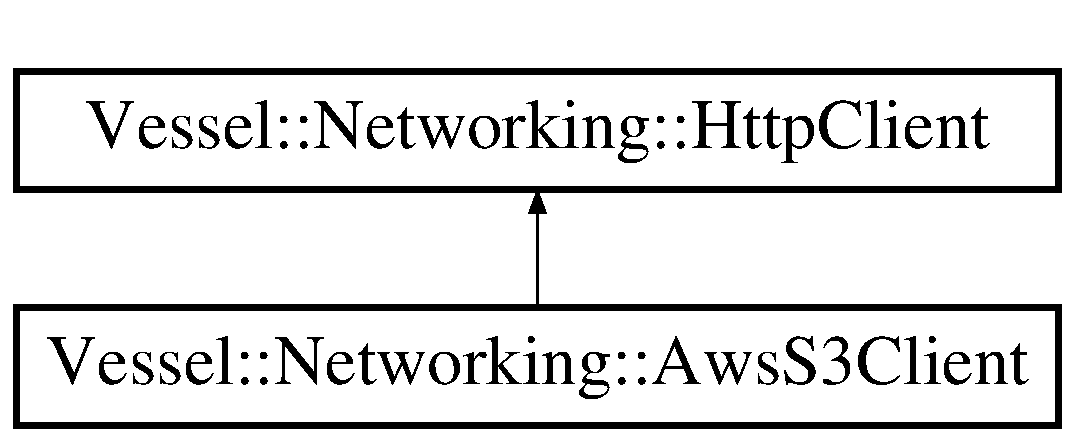
\includegraphics[height=2.000000cm]{class_vessel_1_1_networking_1_1_aws_s3_client}
\end{center}
\end{figure}
\subsection*{Public Types}
\begin{DoxyCompactItemize}
\item 
\mbox{\Hypertarget{class_vessel_1_1_networking_1_1_aws_s3_client_a0dd37e7d17b27a7772cc0534c5bd5537}\label{class_vessel_1_1_networking_1_1_aws_s3_client_a0dd37e7d17b27a7772cc0534c5bd5537}} 
enum {\bfseries Aws\+Flags} \{ \newline
{\bfseries No\+Flags} = 0, 
{\bfseries Reduced\+Redundancy} = 1, 
{\bfseries Multipart} = 2, 
{\bfseries Streaming} = 4, 
\newline
{\bfseries Encrypted} = 6, 
{\bfseries Skip\+Multi\+Init} = 8
 \}
\end{DoxyCompactItemize}
\subsection*{Public Member Functions}
\begin{DoxyCompactItemize}
\item 
\mbox{\Hypertarget{class_vessel_1_1_networking_1_1_aws_s3_client_a298d769b7ef2478a29eb7289039e67e2}\label{class_vessel_1_1_networking_1_1_aws_s3_client_a298d769b7ef2478a29eb7289039e67e2}} 
{\bfseries Aws\+S3\+Client} (const \hyperlink{struct_vessel_1_1_types_1_1_storage_provider}{Storage\+Provider} \&provider)
\item 
\mbox{\Hypertarget{class_vessel_1_1_networking_1_1_aws_s3_client_a50dc6763024104c359dfca61ae3e2f90}\label{class_vessel_1_1_networking_1_1_aws_s3_client_a50dc6763024104c359dfca61ae3e2f90}} 
void {\bfseries set\+\_\+http\+\_\+request} (const \hyperlink{class_vessel_1_1_networking_1_1_http_request}{Http\+Request} \&r)
\item 
bool \hyperlink{class_vessel_1_1_networking_1_1_aws_s3_client_a2e08698221d54ca88ac5055d991eb21f}{init\+\_\+upload} (const \hyperlink{class_vessel_1_1_file_1_1_backup_file}{Backup\+File} \&bf, Aws\+Flags flags=Aws\+Flags\+::\+Reduced\+Redundancy)
\begin{DoxyCompactList}\small\item\em Initializes the A\+WS S3 upload. \end{DoxyCompactList}\item 
\mbox{\Hypertarget{class_vessel_1_1_networking_1_1_aws_s3_client_ab9e7eb4b95cece8a1283d12d9e72b55c}\label{class_vessel_1_1_networking_1_1_aws_s3_client_ab9e7eb4b95cece8a1283d12d9e72b55c}} 
void \hyperlink{class_vessel_1_1_networking_1_1_aws_s3_client_ab9e7eb4b95cece8a1283d12d9e72b55c}{set\+\_\+part\+\_\+size} (size\+\_\+t part\+\_\+size)
\begin{DoxyCompactList}\small\item\em Sets the part size in bytes for multipart uploads. \end{DoxyCompactList}\item 
bool \hyperlink{class_vessel_1_1_networking_1_1_aws_s3_client_ae78ce420213ab93e81b6fee0911c4746}{upload} ()
\begin{DoxyCompactList}\small\item\em Uploads a single file to the A\+WS S3 R\+E\+ST A\+PI. \end{DoxyCompactList}\item 
std\+::string \hyperlink{class_vessel_1_1_networking_1_1_aws_s3_client_a2588b9b6a22ea6610e4a4eddec2973de}{upload\+\_\+part} (int part\+\_\+number, const std\+::string \&upload\+\_\+id)
\begin{DoxyCompactList}\small\item\em Uploads a single file to the A\+WS S3 R\+E\+ST A\+PI. \end{DoxyCompactList}\item 
std\+::string \hyperlink{class_vessel_1_1_networking_1_1_aws_s3_client_add76f620364375f1a54730175e869de9}{complete\+\_\+multipart\+\_\+upload} (const std\+::vector$<$ \hyperlink{struct_vessel_1_1_types_1_1_upload_tag_set}{Upload\+Tag\+Set} $>$ \&etags, const std\+::string \&upload\+\_\+id)
\begin{DoxyCompactList}\small\item\em Completes a multipart upload and returns the E\+Tag for the file upload. \end{DoxyCompactList}\item 
bool \hyperlink{class_vessel_1_1_networking_1_1_aws_s3_client_aa5d5c62b27ceb78262a33d835abaa8be}{upload\+\_\+stream\+\_\+chunk} (int part\+\_\+number, const std\+::string \&prev\+\_\+signature)
\begin{DoxyCompactList}\small\item\em Streaming file upload to the A\+WS S3 R\+E\+ST A\+PI. \end{DoxyCompactList}\item 
std\+::string \hyperlink{class_vessel_1_1_networking_1_1_aws_s3_client_ad606a5dd675054cbf1598d662ff90443}{get\+\_\+last\+\_\+signature} ()
\begin{DoxyCompactList}\small\item\em Returns the signature for the previous upload part. \end{DoxyCompactList}\item 
std\+::string \hyperlink{class_vessel_1_1_networking_1_1_aws_s3_client_af255a5ea67ccd234e90518d149737603}{get\+\_\+upload\+\_\+id} ()
\begin{DoxyCompactList}\small\item\em Returns the upload ID for Multipart uploads. \end{DoxyCompactList}\item 
\mbox{\Hypertarget{class_vessel_1_1_networking_1_1_aws_s3_client_a71ddd6a81d15eec7e5423cee6d064451}\label{class_vessel_1_1_networking_1_1_aws_s3_client_a71ddd6a81d15eec7e5423cee6d064451}} 
void \hyperlink{class_vessel_1_1_networking_1_1_aws_s3_client_a71ddd6a81d15eec7e5423cee6d064451}{set\+\_\+upload\+\_\+id} (const std\+::string \&upload\+\_\+id)
\begin{DoxyCompactList}\small\item\em Sets the upload id of the A\+WS S3 upload. Can be used for resuming uploads or performing other operations. \end{DoxyCompactList}\item 
\mbox{\Hypertarget{class_vessel_1_1_networking_1_1_aws_s3_client_a947727d7f26407fafd7c5987e1a68c88}\label{class_vessel_1_1_networking_1_1_aws_s3_client_a947727d7f26407fafd7c5987e1a68c88}} 
void \hyperlink{class_vessel_1_1_networking_1_1_aws_s3_client_a947727d7f26407fafd7c5987e1a68c88}{set\+\_\+file} (const \hyperlink{class_vessel_1_1_file_1_1_backup_file}{Backup\+File} \&bf)
\begin{DoxyCompactList}\small\item\em Sets a pointer to the Backup\+File. \end{DoxyCompactList}\item 
\mbox{\Hypertarget{class_vessel_1_1_networking_1_1_aws_s3_client_a5dbe469161a506de0a5e6ec74461328a}\label{class_vessel_1_1_networking_1_1_aws_s3_client_a5dbe469161a506de0a5e6ec74461328a}} 
void \hyperlink{class_vessel_1_1_networking_1_1_aws_s3_client_a5dbe469161a506de0a5e6ec74461328a}{remote\+\_\+signing} (bool flag)
\begin{DoxyCompactList}\small\item\em If enabled, the request will be signed remotely via the Vessel A\+PI. Otherwise, a local key file will be used. \end{DoxyCompactList}\item 
\mbox{\Hypertarget{class_vessel_1_1_networking_1_1_aws_s3_client_a96e454d8d46844fcddc7a72e639aa80e}\label{class_vessel_1_1_networking_1_1_aws_s3_client_a96e454d8d46844fcddc7a72e639aa80e}} 
void \hyperlink{class_vessel_1_1_networking_1_1_aws_s3_client_a96e454d8d46844fcddc7a72e639aa80e}{set\+\_\+storage\+\_\+provider} (const \hyperlink{struct_vessel_1_1_types_1_1_storage_provider}{Storage\+Provider} \&provider)
\begin{DoxyCompactList}\small\item\em Sets the internal storage provider for the A\+WS client. Used for key signing. \end{DoxyCompactList}\item 
std\+::string \hyperlink{class_vessel_1_1_networking_1_1_aws_s3_client_a00d6b781a56662ed5e80c9032fe1c380}{get\+\_\+file\+\_\+uri\+\_\+path} ()
\begin{DoxyCompactList}\small\item\em Returns the relative path to the file on the cloud server. \end{DoxyCompactList}\item 
size\+\_\+t \hyperlink{class_vessel_1_1_networking_1_1_aws_s3_client_ae836c56e69d9ac911f660d0c4d8d0ebc}{get\+\_\+current\+\_\+part\+\_\+size} ()
\begin{DoxyCompactList}\small\item\em Returns the total size in bytes of the current part to be uploaded. \end{DoxyCompactList}\end{DoxyCompactItemize}
\subsection*{Friends}
\begin{DoxyCompactItemize}
\item 
\mbox{\Hypertarget{class_vessel_1_1_networking_1_1_aws_s3_client_a65721bc87df7845108fc1d6bffee63f7}\label{class_vessel_1_1_networking_1_1_aws_s3_client_a65721bc87df7845108fc1d6bffee63f7}} 
Aws\+Flags {\bfseries operator$\vert$} (Aws\+Flags a, Aws\+Flags b)
\item 
\mbox{\Hypertarget{class_vessel_1_1_networking_1_1_aws_s3_client_acf095f8ff202c0997eb2c85460498f56}\label{class_vessel_1_1_networking_1_1_aws_s3_client_acf095f8ff202c0997eb2c85460498f56}} 
Aws\+Flags {\bfseries operator \&} (Aws\+Flags a, Aws\+Flags b)
\end{DoxyCompactItemize}
\subsection*{Additional Inherited Members}


\subsection{Member Function Documentation}
\mbox{\Hypertarget{class_vessel_1_1_networking_1_1_aws_s3_client_add76f620364375f1a54730175e869de9}\label{class_vessel_1_1_networking_1_1_aws_s3_client_add76f620364375f1a54730175e869de9}} 
\index{Vessel\+::\+Networking\+::\+Aws\+S3\+Client@{Vessel\+::\+Networking\+::\+Aws\+S3\+Client}!complete\+\_\+multipart\+\_\+upload@{complete\+\_\+multipart\+\_\+upload}}
\index{complete\+\_\+multipart\+\_\+upload@{complete\+\_\+multipart\+\_\+upload}!Vessel\+::\+Networking\+::\+Aws\+S3\+Client@{Vessel\+::\+Networking\+::\+Aws\+S3\+Client}}
\subsubsection{\texorpdfstring{complete\+\_\+multipart\+\_\+upload()}{complete\_multipart\_upload()}}
{\footnotesize\ttfamily std\+::string Vessel\+::\+Networking\+::\+Aws\+S3\+Client\+::complete\+\_\+multipart\+\_\+upload (\begin{DoxyParamCaption}\item[{const std\+::vector$<$ \hyperlink{struct_vessel_1_1_types_1_1_upload_tag_set}{Upload\+Tag\+Set} $>$ \&}]{etags,  }\item[{const std\+::string \&}]{upload\+\_\+id }\end{DoxyParamCaption})}



Completes a multipart upload and returns the E\+Tag for the file upload. 

\begin{DoxyReturn}{Returns}
Completes a multipart upload and returns the E\+Tag for the file upload 
\end{DoxyReturn}
\mbox{\Hypertarget{class_vessel_1_1_networking_1_1_aws_s3_client_ae836c56e69d9ac911f660d0c4d8d0ebc}\label{class_vessel_1_1_networking_1_1_aws_s3_client_ae836c56e69d9ac911f660d0c4d8d0ebc}} 
\index{Vessel\+::\+Networking\+::\+Aws\+S3\+Client@{Vessel\+::\+Networking\+::\+Aws\+S3\+Client}!get\+\_\+current\+\_\+part\+\_\+size@{get\+\_\+current\+\_\+part\+\_\+size}}
\index{get\+\_\+current\+\_\+part\+\_\+size@{get\+\_\+current\+\_\+part\+\_\+size}!Vessel\+::\+Networking\+::\+Aws\+S3\+Client@{Vessel\+::\+Networking\+::\+Aws\+S3\+Client}}
\subsubsection{\texorpdfstring{get\+\_\+current\+\_\+part\+\_\+size()}{get\_current\_part\_size()}}
{\footnotesize\ttfamily size\+\_\+t Vessel\+::\+Networking\+::\+Aws\+S3\+Client\+::get\+\_\+current\+\_\+part\+\_\+size (\begin{DoxyParamCaption}{ }\end{DoxyParamCaption})}



Returns the total size in bytes of the current part to be uploaded. 

\begin{DoxyReturn}{Returns}
Returns the total size in bytes of the current part to be uploaded 
\end{DoxyReturn}
\mbox{\Hypertarget{class_vessel_1_1_networking_1_1_aws_s3_client_a00d6b781a56662ed5e80c9032fe1c380}\label{class_vessel_1_1_networking_1_1_aws_s3_client_a00d6b781a56662ed5e80c9032fe1c380}} 
\index{Vessel\+::\+Networking\+::\+Aws\+S3\+Client@{Vessel\+::\+Networking\+::\+Aws\+S3\+Client}!get\+\_\+file\+\_\+uri\+\_\+path@{get\+\_\+file\+\_\+uri\+\_\+path}}
\index{get\+\_\+file\+\_\+uri\+\_\+path@{get\+\_\+file\+\_\+uri\+\_\+path}!Vessel\+::\+Networking\+::\+Aws\+S3\+Client@{Vessel\+::\+Networking\+::\+Aws\+S3\+Client}}
\subsubsection{\texorpdfstring{get\+\_\+file\+\_\+uri\+\_\+path()}{get\_file\_uri\_path()}}
{\footnotesize\ttfamily std\+::string Vessel\+::\+Networking\+::\+Aws\+S3\+Client\+::get\+\_\+file\+\_\+uri\+\_\+path (\begin{DoxyParamCaption}{ }\end{DoxyParamCaption})}



Returns the relative path to the file on the cloud server. 

\begin{DoxyReturn}{Returns}
Returns the relative path to the file on the cloud server 
\end{DoxyReturn}
\mbox{\Hypertarget{class_vessel_1_1_networking_1_1_aws_s3_client_ad606a5dd675054cbf1598d662ff90443}\label{class_vessel_1_1_networking_1_1_aws_s3_client_ad606a5dd675054cbf1598d662ff90443}} 
\index{Vessel\+::\+Networking\+::\+Aws\+S3\+Client@{Vessel\+::\+Networking\+::\+Aws\+S3\+Client}!get\+\_\+last\+\_\+signature@{get\+\_\+last\+\_\+signature}}
\index{get\+\_\+last\+\_\+signature@{get\+\_\+last\+\_\+signature}!Vessel\+::\+Networking\+::\+Aws\+S3\+Client@{Vessel\+::\+Networking\+::\+Aws\+S3\+Client}}
\subsubsection{\texorpdfstring{get\+\_\+last\+\_\+signature()}{get\_last\_signature()}}
{\footnotesize\ttfamily std\+::string Vessel\+::\+Networking\+::\+Aws\+S3\+Client\+::get\+\_\+last\+\_\+signature (\begin{DoxyParamCaption}{ }\end{DoxyParamCaption})}



Returns the signature for the previous upload part. 

\begin{DoxyReturn}{Returns}
Returns the signature for the previous upload part 
\end{DoxyReturn}
\mbox{\Hypertarget{class_vessel_1_1_networking_1_1_aws_s3_client_af255a5ea67ccd234e90518d149737603}\label{class_vessel_1_1_networking_1_1_aws_s3_client_af255a5ea67ccd234e90518d149737603}} 
\index{Vessel\+::\+Networking\+::\+Aws\+S3\+Client@{Vessel\+::\+Networking\+::\+Aws\+S3\+Client}!get\+\_\+upload\+\_\+id@{get\+\_\+upload\+\_\+id}}
\index{get\+\_\+upload\+\_\+id@{get\+\_\+upload\+\_\+id}!Vessel\+::\+Networking\+::\+Aws\+S3\+Client@{Vessel\+::\+Networking\+::\+Aws\+S3\+Client}}
\subsubsection{\texorpdfstring{get\+\_\+upload\+\_\+id()}{get\_upload\_id()}}
{\footnotesize\ttfamily std\+::string Vessel\+::\+Networking\+::\+Aws\+S3\+Client\+::get\+\_\+upload\+\_\+id (\begin{DoxyParamCaption}{ }\end{DoxyParamCaption})}



Returns the upload ID for Multipart uploads. 

\begin{DoxyReturn}{Returns}
Returns the upload ID for Multipart uploads 
\end{DoxyReturn}
\mbox{\Hypertarget{class_vessel_1_1_networking_1_1_aws_s3_client_a2e08698221d54ca88ac5055d991eb21f}\label{class_vessel_1_1_networking_1_1_aws_s3_client_a2e08698221d54ca88ac5055d991eb21f}} 
\index{Vessel\+::\+Networking\+::\+Aws\+S3\+Client@{Vessel\+::\+Networking\+::\+Aws\+S3\+Client}!init\+\_\+upload@{init\+\_\+upload}}
\index{init\+\_\+upload@{init\+\_\+upload}!Vessel\+::\+Networking\+::\+Aws\+S3\+Client@{Vessel\+::\+Networking\+::\+Aws\+S3\+Client}}
\subsubsection{\texorpdfstring{init\+\_\+upload()}{init\_upload()}}
{\footnotesize\ttfamily bool Vessel\+::\+Networking\+::\+Aws\+S3\+Client\+::init\+\_\+upload (\begin{DoxyParamCaption}\item[{const \hyperlink{class_vessel_1_1_file_1_1_backup_file}{Backup\+File} \&}]{bf,  }\item[{Aws\+Flags}]{flags = {\ttfamily AwsFlags\+:\+:ReducedRedundancy} }\end{DoxyParamCaption})}



Initializes the A\+WS S3 upload. 

\begin{DoxyReturn}{Returns}
Returns true if the upload was initialized 
\end{DoxyReturn}
\mbox{\Hypertarget{class_vessel_1_1_networking_1_1_aws_s3_client_ae78ce420213ab93e81b6fee0911c4746}\label{class_vessel_1_1_networking_1_1_aws_s3_client_ae78ce420213ab93e81b6fee0911c4746}} 
\index{Vessel\+::\+Networking\+::\+Aws\+S3\+Client@{Vessel\+::\+Networking\+::\+Aws\+S3\+Client}!upload@{upload}}
\index{upload@{upload}!Vessel\+::\+Networking\+::\+Aws\+S3\+Client@{Vessel\+::\+Networking\+::\+Aws\+S3\+Client}}
\subsubsection{\texorpdfstring{upload()}{upload()}}
{\footnotesize\ttfamily bool Vessel\+::\+Networking\+::\+Aws\+S3\+Client\+::upload (\begin{DoxyParamCaption}{ }\end{DoxyParamCaption})}



Uploads a single file to the A\+WS S3 R\+E\+ST A\+PI. 

\begin{DoxyReturn}{Returns}
Returns true if the upload was successful, or false if there was an error 
\end{DoxyReturn}
\mbox{\Hypertarget{class_vessel_1_1_networking_1_1_aws_s3_client_a2588b9b6a22ea6610e4a4eddec2973de}\label{class_vessel_1_1_networking_1_1_aws_s3_client_a2588b9b6a22ea6610e4a4eddec2973de}} 
\index{Vessel\+::\+Networking\+::\+Aws\+S3\+Client@{Vessel\+::\+Networking\+::\+Aws\+S3\+Client}!upload\+\_\+part@{upload\+\_\+part}}
\index{upload\+\_\+part@{upload\+\_\+part}!Vessel\+::\+Networking\+::\+Aws\+S3\+Client@{Vessel\+::\+Networking\+::\+Aws\+S3\+Client}}
\subsubsection{\texorpdfstring{upload\+\_\+part()}{upload\_part()}}
{\footnotesize\ttfamily std\+::string Vessel\+::\+Networking\+::\+Aws\+S3\+Client\+::upload\+\_\+part (\begin{DoxyParamCaption}\item[{int}]{part\+\_\+number,  }\item[{const std\+::string \&}]{upload\+\_\+id }\end{DoxyParamCaption})}



Uploads a single file to the A\+WS S3 R\+E\+ST A\+PI. 

\begin{DoxyReturn}{Returns}
Returns the Etag for the upload part if successful 
\end{DoxyReturn}
\mbox{\Hypertarget{class_vessel_1_1_networking_1_1_aws_s3_client_aa5d5c62b27ceb78262a33d835abaa8be}\label{class_vessel_1_1_networking_1_1_aws_s3_client_aa5d5c62b27ceb78262a33d835abaa8be}} 
\index{Vessel\+::\+Networking\+::\+Aws\+S3\+Client@{Vessel\+::\+Networking\+::\+Aws\+S3\+Client}!upload\+\_\+stream\+\_\+chunk@{upload\+\_\+stream\+\_\+chunk}}
\index{upload\+\_\+stream\+\_\+chunk@{upload\+\_\+stream\+\_\+chunk}!Vessel\+::\+Networking\+::\+Aws\+S3\+Client@{Vessel\+::\+Networking\+::\+Aws\+S3\+Client}}
\subsubsection{\texorpdfstring{upload\+\_\+stream\+\_\+chunk()}{upload\_stream\_chunk()}}
{\footnotesize\ttfamily bool Vessel\+::\+Networking\+::\+Aws\+S3\+Client\+::upload\+\_\+stream\+\_\+chunk (\begin{DoxyParamCaption}\item[{int}]{part\+\_\+number,  }\item[{const std\+::string \&}]{prev\+\_\+signature }\end{DoxyParamCaption})}



Streaming file upload to the A\+WS S3 R\+E\+ST A\+PI. 

\begin{DoxyReturn}{Returns}
Returns true if the upload was successful, or false if there was an error 
\end{DoxyReturn}


The documentation for this class was generated from the following file\+:\begin{DoxyCompactItemize}
\item 
/home/kyle/cpp/bv-\/backup/include/vessel/aws/aws\+\_\+s3\+\_\+client.\+hpp\end{DoxyCompactItemize}

\hypertarget{class_vessel_1_1_aws_upload}{}\section{Vessel\+:\+:Aws\+Upload Class Reference}
\label{class_vessel_1_1_aws_upload}\index{Vessel\+::\+Aws\+Upload@{Vessel\+::\+Aws\+Upload}}
Inheritance diagram for Vessel\+:\+:Aws\+Upload\+:\begin{figure}[H]
\begin{center}
\leavevmode
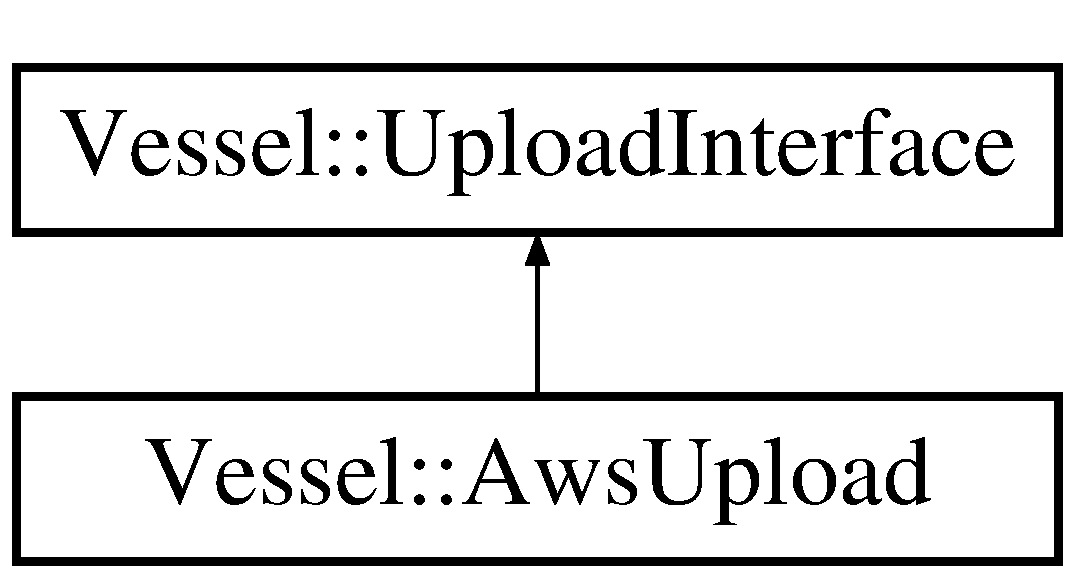
\includegraphics[height=2.000000cm]{class_vessel_1_1_aws_upload}
\end{center}
\end{figure}
\subsection*{Public Member Functions}
\begin{DoxyCompactItemize}
\item 
\mbox{\Hypertarget{class_vessel_1_1_aws_upload_a4c62bfe4e9ff4f99bebcdc0dd1a8b425}\label{class_vessel_1_1_aws_upload_a4c62bfe4e9ff4f99bebcdc0dd1a8b425}} 
void {\bfseries upload\+\_\+file} (\hyperlink{class_vessel_1_1_file_1_1_file_upload}{File\+Upload} \&upload)
\item 
\mbox{\Hypertarget{class_vessel_1_1_aws_upload_a3aaf42e744ed947da06589690ac5dd46}\label{class_vessel_1_1_aws_upload_a3aaf42e744ed947da06589690ac5dd46}} 
void {\bfseries resume\+\_\+uploads} ()
\item 
\mbox{\Hypertarget{class_vessel_1_1_aws_upload_a96d6baa1123cc73a4b7be1446d30387d}\label{class_vessel_1_1_aws_upload_a96d6baa1123cc73a4b7be1446d30387d}} 
void {\bfseries complete\+\_\+upload} ()
\end{DoxyCompactItemize}
\subsection*{Additional Inherited Members}


The documentation for this class was generated from the following file\+:\begin{DoxyCompactItemize}
\item 
/home/kyle/cpp/bv-\/backup/include/vessel/vessel/upload\+\_\+manager.\+hpp\end{DoxyCompactItemize}

\hypertarget{class_vessel_1_1_networking_1_1_azure_client}{}\section{Vessel\+:\+:Networking\+:\+:Azure\+Client Class Reference}
\label{class_vessel_1_1_networking_1_1_azure_client}\index{Vessel\+::\+Networking\+::\+Azure\+Client@{Vessel\+::\+Networking\+::\+Azure\+Client}}
Inheritance diagram for Vessel\+:\+:Networking\+:\+:Azure\+Client\+:\begin{figure}[H]
\begin{center}
\leavevmode
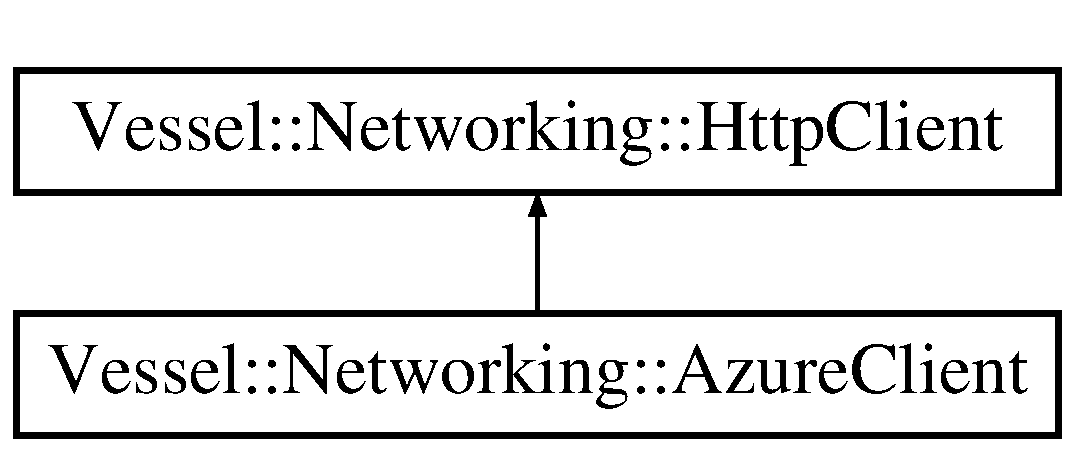
\includegraphics[height=2.000000cm]{class_vessel_1_1_networking_1_1_azure_client}
\end{center}
\end{figure}
\subsection*{Public Member Functions}
\begin{DoxyCompactItemize}
\item 
\mbox{\Hypertarget{class_vessel_1_1_networking_1_1_azure_client_af23230f150558566932d144f335b983f}\label{class_vessel_1_1_networking_1_1_azure_client_af23230f150558566932d144f335b983f}} 
{\bfseries Azure\+Client} (const \hyperlink{struct_vessel_1_1_types_1_1_storage_provider}{Storage\+Provider} \&provider)
\item 
\mbox{\Hypertarget{class_vessel_1_1_networking_1_1_azure_client_a1618ca5045621c283d09b9deaf69d467}\label{class_vessel_1_1_networking_1_1_azure_client_a1618ca5045621c283d09b9deaf69d467}} 
void \hyperlink{class_vessel_1_1_networking_1_1_azure_client_a1618ca5045621c283d09b9deaf69d467}{init\+\_\+upload} (const \hyperlink{class_vessel_1_1_file_1_1_backup_file}{Backup\+File} \&file)
\begin{DoxyCompactList}\small\item\em Initializes the Azure upload. \end{DoxyCompactList}\item 
\mbox{\Hypertarget{class_vessel_1_1_networking_1_1_azure_client_a3cc612beede266147a30d4cf1b02ed0e}\label{class_vessel_1_1_networking_1_1_azure_client_a3cc612beede266147a30d4cf1b02ed0e}} 
bool \hyperlink{class_vessel_1_1_networking_1_1_azure_client_a3cc612beede266147a30d4cf1b02ed0e}{init\+\_\+block} ()
\begin{DoxyCompactList}\small\item\em Initializes a multi block upload. \end{DoxyCompactList}\item 
bool \hyperlink{class_vessel_1_1_networking_1_1_azure_client_aea048602d61d1701883483b394c7a4d8}{upload} ()
\begin{DoxyCompactList}\small\item\em Uploads a single file to the Azure Storage A\+PI. \end{DoxyCompactList}\item 
bool \hyperlink{class_vessel_1_1_networking_1_1_azure_client_ae1b65c7d173d3592f0ab8b3fab80bebc}{upload\+\_\+part} (int part\+\_\+number)
\begin{DoxyCompactList}\small\item\em Uploads a blob block. \end{DoxyCompactList}\item 
bool \hyperlink{class_vessel_1_1_networking_1_1_azure_client_abfcd51780d84a5b4f7735fd18bca08ec}{complete\+\_\+multipart\+\_\+upload} (int total\+\_\+parts)
\begin{DoxyCompactList}\small\item\em Completes a multipart (block) upload. \end{DoxyCompactList}\item 
std\+::string \hyperlink{class_vessel_1_1_networking_1_1_azure_client_a103016ab4521dacb9e6b7c24a2c3496a}{get\+\_\+block\+\_\+list} ()
\begin{DoxyCompactList}\small\item\em Returns the block list for the current blob. \end{DoxyCompactList}\item 
\mbox{\Hypertarget{class_vessel_1_1_networking_1_1_azure_client_a65eb07517634e97d9a180eb4d429bce2}\label{class_vessel_1_1_networking_1_1_azure_client_a65eb07517634e97d9a180eb4d429bce2}} 
void \hyperlink{class_vessel_1_1_networking_1_1_azure_client_a65eb07517634e97d9a180eb4d429bce2}{remote\+\_\+signing} (bool flag)
\begin{DoxyCompactList}\small\item\em Enables or disables remote signing the request. Local key file is used for local. \end{DoxyCompactList}\item 
std\+::string \hyperlink{class_vessel_1_1_networking_1_1_azure_client_aabdd68349e22f2124804d725bde09123}{last\+\_\+request\+\_\+id} ()
\begin{DoxyCompactList}\small\item\em Returns the last Azure request id. \end{DoxyCompactList}\item 
std\+::string \hyperlink{class_vessel_1_1_networking_1_1_azure_client_a74e4cfe536c3099aadf1c8df785f53d4}{get\+\_\+upload\+\_\+id} ()
\begin{DoxyCompactList}\small\item\em Returns the upload ID for Azure Blob Upload. \end{DoxyCompactList}\item 
\mbox{\Hypertarget{class_vessel_1_1_networking_1_1_azure_client_a73021b3608871fe36a0172d0481f0e53}\label{class_vessel_1_1_networking_1_1_azure_client_a73021b3608871fe36a0172d0481f0e53}} 
void \hyperlink{class_vessel_1_1_networking_1_1_azure_client_a73021b3608871fe36a0172d0481f0e53}{set\+\_\+upload\+\_\+id} (const std\+::string \&upload\+\_\+id)
\begin{DoxyCompactList}\small\item\em Sets the upload/request id of the current Azure Blob upload. \end{DoxyCompactList}\item 
std\+::string \hyperlink{class_vessel_1_1_networking_1_1_azure_client_ae2c4d287ee5c326380c426a91dae7b23}{get\+\_\+padded\+\_\+block\+\_\+id} (const std\+::string \&id)
\begin{DoxyCompactList}\small\item\em Pads the block id (integer part number) by leading zeroes. \end{DoxyCompactList}\end{DoxyCompactItemize}
\subsection*{Additional Inherited Members}


\subsection{Member Function Documentation}
\mbox{\Hypertarget{class_vessel_1_1_networking_1_1_azure_client_abfcd51780d84a5b4f7735fd18bca08ec}\label{class_vessel_1_1_networking_1_1_azure_client_abfcd51780d84a5b4f7735fd18bca08ec}} 
\index{Vessel\+::\+Networking\+::\+Azure\+Client@{Vessel\+::\+Networking\+::\+Azure\+Client}!complete\+\_\+multipart\+\_\+upload@{complete\+\_\+multipart\+\_\+upload}}
\index{complete\+\_\+multipart\+\_\+upload@{complete\+\_\+multipart\+\_\+upload}!Vessel\+::\+Networking\+::\+Azure\+Client@{Vessel\+::\+Networking\+::\+Azure\+Client}}
\subsubsection{\texorpdfstring{complete\+\_\+multipart\+\_\+upload()}{complete\_multipart\_upload()}}
{\footnotesize\ttfamily bool Vessel\+::\+Networking\+::\+Azure\+Client\+::complete\+\_\+multipart\+\_\+upload (\begin{DoxyParamCaption}\item[{int}]{total\+\_\+parts }\end{DoxyParamCaption})}



Completes a multipart (block) upload. 

\begin{DoxyReturn}{Returns}
Returns true if the operation was successful 
\end{DoxyReturn}
\mbox{\Hypertarget{class_vessel_1_1_networking_1_1_azure_client_a103016ab4521dacb9e6b7c24a2c3496a}\label{class_vessel_1_1_networking_1_1_azure_client_a103016ab4521dacb9e6b7c24a2c3496a}} 
\index{Vessel\+::\+Networking\+::\+Azure\+Client@{Vessel\+::\+Networking\+::\+Azure\+Client}!get\+\_\+block\+\_\+list@{get\+\_\+block\+\_\+list}}
\index{get\+\_\+block\+\_\+list@{get\+\_\+block\+\_\+list}!Vessel\+::\+Networking\+::\+Azure\+Client@{Vessel\+::\+Networking\+::\+Azure\+Client}}
\subsubsection{\texorpdfstring{get\+\_\+block\+\_\+list()}{get\_block\_list()}}
{\footnotesize\ttfamily std\+::string Vessel\+::\+Networking\+::\+Azure\+Client\+::get\+\_\+block\+\_\+list (\begin{DoxyParamCaption}{ }\end{DoxyParamCaption})}



Returns the block list for the current blob. 

\begin{DoxyReturn}{Returns}
Returns the block list for the current blob 
\end{DoxyReturn}
\mbox{\Hypertarget{class_vessel_1_1_networking_1_1_azure_client_ae2c4d287ee5c326380c426a91dae7b23}\label{class_vessel_1_1_networking_1_1_azure_client_ae2c4d287ee5c326380c426a91dae7b23}} 
\index{Vessel\+::\+Networking\+::\+Azure\+Client@{Vessel\+::\+Networking\+::\+Azure\+Client}!get\+\_\+padded\+\_\+block\+\_\+id@{get\+\_\+padded\+\_\+block\+\_\+id}}
\index{get\+\_\+padded\+\_\+block\+\_\+id@{get\+\_\+padded\+\_\+block\+\_\+id}!Vessel\+::\+Networking\+::\+Azure\+Client@{Vessel\+::\+Networking\+::\+Azure\+Client}}
\subsubsection{\texorpdfstring{get\+\_\+padded\+\_\+block\+\_\+id()}{get\_padded\_block\_id()}}
{\footnotesize\ttfamily std\+::string Vessel\+::\+Networking\+::\+Azure\+Client\+::get\+\_\+padded\+\_\+block\+\_\+id (\begin{DoxyParamCaption}\item[{const std\+::string \&}]{id }\end{DoxyParamCaption})}



Pads the block id (integer part number) by leading zeroes. 

\begin{DoxyReturn}{Returns}
R\+Pads the block id (integer part number) by leading zeroes 
\end{DoxyReturn}
\mbox{\Hypertarget{class_vessel_1_1_networking_1_1_azure_client_a74e4cfe536c3099aadf1c8df785f53d4}\label{class_vessel_1_1_networking_1_1_azure_client_a74e4cfe536c3099aadf1c8df785f53d4}} 
\index{Vessel\+::\+Networking\+::\+Azure\+Client@{Vessel\+::\+Networking\+::\+Azure\+Client}!get\+\_\+upload\+\_\+id@{get\+\_\+upload\+\_\+id}}
\index{get\+\_\+upload\+\_\+id@{get\+\_\+upload\+\_\+id}!Vessel\+::\+Networking\+::\+Azure\+Client@{Vessel\+::\+Networking\+::\+Azure\+Client}}
\subsubsection{\texorpdfstring{get\+\_\+upload\+\_\+id()}{get\_upload\_id()}}
{\footnotesize\ttfamily std\+::string Vessel\+::\+Networking\+::\+Azure\+Client\+::get\+\_\+upload\+\_\+id (\begin{DoxyParamCaption}{ }\end{DoxyParamCaption})}



Returns the upload ID for Azure Blob Upload. 

\begin{DoxyReturn}{Returns}
Returns the upload ID for the Azure Blob Upload 
\end{DoxyReturn}
\mbox{\Hypertarget{class_vessel_1_1_networking_1_1_azure_client_aabdd68349e22f2124804d725bde09123}\label{class_vessel_1_1_networking_1_1_azure_client_aabdd68349e22f2124804d725bde09123}} 
\index{Vessel\+::\+Networking\+::\+Azure\+Client@{Vessel\+::\+Networking\+::\+Azure\+Client}!last\+\_\+request\+\_\+id@{last\+\_\+request\+\_\+id}}
\index{last\+\_\+request\+\_\+id@{last\+\_\+request\+\_\+id}!Vessel\+::\+Networking\+::\+Azure\+Client@{Vessel\+::\+Networking\+::\+Azure\+Client}}
\subsubsection{\texorpdfstring{last\+\_\+request\+\_\+id()}{last\_request\_id()}}
{\footnotesize\ttfamily std\+::string Vessel\+::\+Networking\+::\+Azure\+Client\+::last\+\_\+request\+\_\+id (\begin{DoxyParamCaption}{ }\end{DoxyParamCaption})}



Returns the last Azure request id. 

\begin{DoxyReturn}{Returns}
Returns the last Azure request id 
\end{DoxyReturn}
\mbox{\Hypertarget{class_vessel_1_1_networking_1_1_azure_client_aea048602d61d1701883483b394c7a4d8}\label{class_vessel_1_1_networking_1_1_azure_client_aea048602d61d1701883483b394c7a4d8}} 
\index{Vessel\+::\+Networking\+::\+Azure\+Client@{Vessel\+::\+Networking\+::\+Azure\+Client}!upload@{upload}}
\index{upload@{upload}!Vessel\+::\+Networking\+::\+Azure\+Client@{Vessel\+::\+Networking\+::\+Azure\+Client}}
\subsubsection{\texorpdfstring{upload()}{upload()}}
{\footnotesize\ttfamily bool Vessel\+::\+Networking\+::\+Azure\+Client\+::upload (\begin{DoxyParamCaption}{ }\end{DoxyParamCaption})}



Uploads a single file to the Azure Storage A\+PI. 

\begin{DoxyReturn}{Returns}
Returns true if the upload was successful, or false if there was an error 
\end{DoxyReturn}
\mbox{\Hypertarget{class_vessel_1_1_networking_1_1_azure_client_ae1b65c7d173d3592f0ab8b3fab80bebc}\label{class_vessel_1_1_networking_1_1_azure_client_ae1b65c7d173d3592f0ab8b3fab80bebc}} 
\index{Vessel\+::\+Networking\+::\+Azure\+Client@{Vessel\+::\+Networking\+::\+Azure\+Client}!upload\+\_\+part@{upload\+\_\+part}}
\index{upload\+\_\+part@{upload\+\_\+part}!Vessel\+::\+Networking\+::\+Azure\+Client@{Vessel\+::\+Networking\+::\+Azure\+Client}}
\subsubsection{\texorpdfstring{upload\+\_\+part()}{upload\_part()}}
{\footnotesize\ttfamily bool Vessel\+::\+Networking\+::\+Azure\+Client\+::upload\+\_\+part (\begin{DoxyParamCaption}\item[{int}]{part\+\_\+number }\end{DoxyParamCaption})}



Uploads a blob block. 

\begin{DoxyReturn}{Returns}
Returns true if the operation was success and false otherwise 
\end{DoxyReturn}


The documentation for this class was generated from the following file\+:\begin{DoxyCompactItemize}
\item 
/home/kyle/cpp/bv-\/backup/include/vessel/azure/azure\+\_\+client.\+hpp\end{DoxyCompactItemize}

\hypertarget{class_vessel_1_1_exception_1_1_azure_exception}{}\section{Vessel\+:\+:Exception\+:\+:Azure\+Exception Class Reference}
\label{class_vessel_1_1_exception_1_1_azure_exception}\index{Vessel\+::\+Exception\+::\+Azure\+Exception@{Vessel\+::\+Exception\+::\+Azure\+Exception}}
Inheritance diagram for Vessel\+:\+:Exception\+:\+:Azure\+Exception\+:\begin{figure}[H]
\begin{center}
\leavevmode
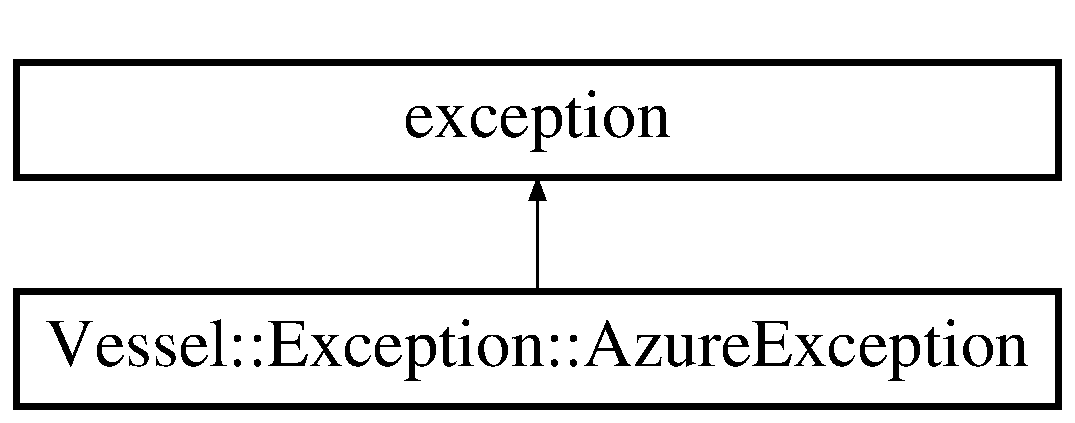
\includegraphics[height=2.000000cm]{class_vessel_1_1_exception_1_1_azure_exception}
\end{center}
\end{figure}
\subsection*{Public Types}
\begin{DoxyCompactItemize}
\item 
\mbox{\Hypertarget{class_vessel_1_1_exception_1_1_azure_exception_a824c85ca9572c0196f1abd738b951d5d}\label{class_vessel_1_1_exception_1_1_azure_exception_a824c85ca9572c0196f1abd738b951d5d}} 
enum {\bfseries Error\+Code} \{ \newline
{\bfseries No\+Error} = 0, 
{\bfseries Bad\+Signature}, 
{\bfseries File\+Not\+Initialized}, 
{\bfseries Init\+Failed}, 
\newline
{\bfseries Upload\+Failed}
 \}
\end{DoxyCompactItemize}
\subsection*{Public Member Functions}
\begin{DoxyCompactItemize}
\item 
\mbox{\Hypertarget{class_vessel_1_1_exception_1_1_azure_exception_ab6773659cc1d95e693f98ad820029a14}\label{class_vessel_1_1_exception_1_1_azure_exception_ab6773659cc1d95e693f98ad820029a14}} 
{\bfseries Azure\+Exception} (Error\+Code e, const std\+::string \&msg)
\item 
\mbox{\Hypertarget{class_vessel_1_1_exception_1_1_azure_exception_a73647882382d7e52aa42b04bf07afa25}\label{class_vessel_1_1_exception_1_1_azure_exception_a73647882382d7e52aa42b04bf07afa25}} 
Error\+Code {\bfseries get\+\_\+code} ()
\item 
\mbox{\Hypertarget{class_vessel_1_1_exception_1_1_azure_exception_a943727ae14ef986550dde9d775ba48d7}\label{class_vessel_1_1_exception_1_1_azure_exception_a943727ae14ef986550dde9d775ba48d7}} 
virtual const char $\ast$ {\bfseries what} () const noexcept override
\end{DoxyCompactItemize}


The documentation for this class was generated from the following file\+:\begin{DoxyCompactItemize}
\item 
/home/kyle/cpp/bv-\/backup/include/vessel/azure/azure\+\_\+exception.\+hpp\end{DoxyCompactItemize}

\hypertarget{class_vessel_1_1_azure_upload}{}\section{Vessel\+:\+:Azure\+Upload Class Reference}
\label{class_vessel_1_1_azure_upload}\index{Vessel\+::\+Azure\+Upload@{Vessel\+::\+Azure\+Upload}}
Inheritance diagram for Vessel\+:\+:Azure\+Upload\+:\begin{figure}[H]
\begin{center}
\leavevmode
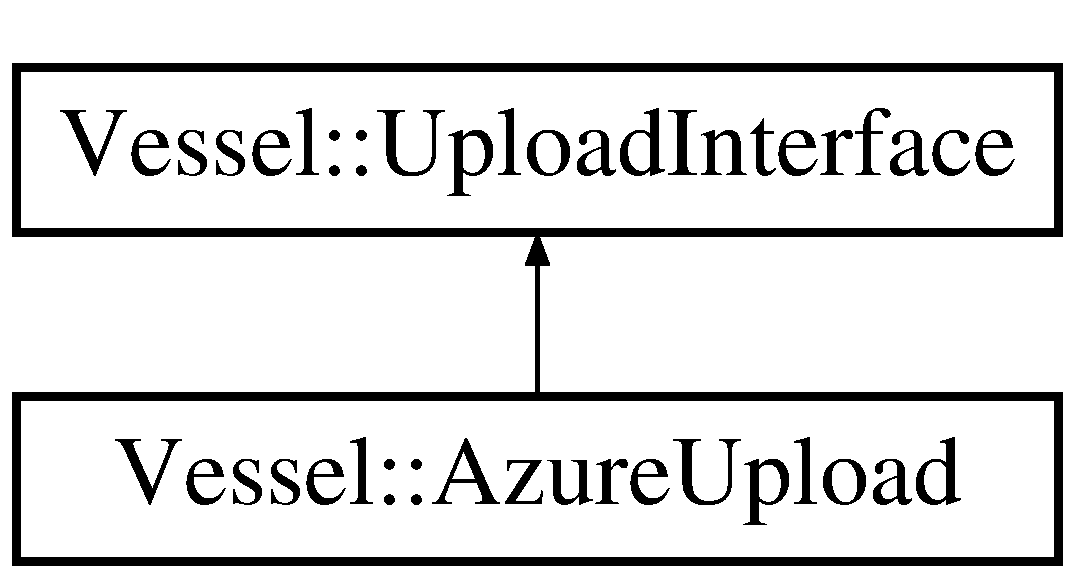
\includegraphics[height=2.000000cm]{class_vessel_1_1_azure_upload}
\end{center}
\end{figure}
\subsection*{Public Member Functions}
\begin{DoxyCompactItemize}
\item 
\mbox{\Hypertarget{class_vessel_1_1_azure_upload_a42a56b9e6dbab4ba1fc68bad4d8806e2}\label{class_vessel_1_1_azure_upload_a42a56b9e6dbab4ba1fc68bad4d8806e2}} 
void {\bfseries upload\+\_\+file} (\hyperlink{class_vessel_1_1_file_1_1_file_upload}{File\+Upload} \&upload)
\item 
\mbox{\Hypertarget{class_vessel_1_1_azure_upload_a26daa8e957193d45238eda00019b4ace}\label{class_vessel_1_1_azure_upload_a26daa8e957193d45238eda00019b4ace}} 
void {\bfseries resume\+\_\+uploads} ()
\item 
\mbox{\Hypertarget{class_vessel_1_1_azure_upload_a42be14aaf7b366bc06733adcc330cf0f}\label{class_vessel_1_1_azure_upload_a42be14aaf7b366bc06733adcc330cf0f}} 
void {\bfseries complete\+\_\+upload} ()
\end{DoxyCompactItemize}
\subsection*{Additional Inherited Members}


The documentation for this class was generated from the following file\+:\begin{DoxyCompactItemize}
\item 
/home/kyle/cpp/bv-\/backup/include/vessel/vessel/upload\+\_\+manager.\+hpp\end{DoxyCompactItemize}

\hypertarget{class_vessel_1_1_file_1_1_backup_directory}{}\section{Vessel\+:\+:File\+:\+:Backup\+Directory Class Reference}
\label{class_vessel_1_1_file_1_1_backup_directory}\index{Vessel\+::\+File\+::\+Backup\+Directory@{Vessel\+::\+File\+::\+Backup\+Directory}}


Helper class for file directories.  




{\ttfamily \#include $<$directory.\+hpp$>$}

\subsection*{Public Member Functions}
\begin{DoxyCompactItemize}
\item 
\mbox{\Hypertarget{class_vessel_1_1_file_1_1_backup_directory_a538c319573c9d0e600550303557f9d71}\label{class_vessel_1_1_file_1_1_backup_directory_a538c319573c9d0e600550303557f9d71}} 
{\bfseries Backup\+Directory} (const boost\+::filesystem\+::path \&fp)
\item 
\mbox{\Hypertarget{class_vessel_1_1_file_1_1_backup_directory_a1e3b4f72745a95cad407eba687e92a1c}\label{class_vessel_1_1_file_1_1_backup_directory_a1e3b4f72745a95cad407eba687e92a1c}} 
{\bfseries Backup\+Directory} (const \hyperlink{class_vessel_1_1_file_1_1_backup_directory}{Backup\+Directory} \&bd)
\item 
\mbox{\Hypertarget{class_vessel_1_1_file_1_1_backup_directory_a73d2cbf7874a46a70cec8ca338caf018}\label{class_vessel_1_1_file_1_1_backup_directory_a73d2cbf7874a46a70cec8ca338caf018}} 
void \hyperlink{class_vessel_1_1_file_1_1_backup_directory_a73d2cbf7874a46a70cec8ca338caf018}{set\+\_\+path} (const std\+::string \&fp)
\begin{DoxyCompactList}\small\item\em Assigns a new directory path to the object. Setting the path triggers all of the associated member attributes and variables to be updated with private method update\+\_\+attributes() \end{DoxyCompactList}\item 
\mbox{\Hypertarget{class_vessel_1_1_file_1_1_backup_directory_a2a3283fa16689b65b32650c8586cd154}\label{class_vessel_1_1_file_1_1_backup_directory_a2a3283fa16689b65b32650c8586cd154}} 
void \hyperlink{class_vessel_1_1_file_1_1_backup_directory_a2a3283fa16689b65b32650c8586cd154}{set\+\_\+path} (const fs\+::path \&file\+\_\+path)
\begin{DoxyCompactList}\small\item\em Assigns a new file path to the object. Setting the path triggers all of the associated member attributes and variables to be updated with private method update\+\_\+attributes() \end{DoxyCompactList}\item 
std\+::string \hyperlink{class_vessel_1_1_file_1_1_backup_directory_a96fda7ffff230b4f3443bfee0dbfe10d}{get\+\_\+dir\+\_\+name} () const
\item 
size\+\_\+t \hyperlink{class_vessel_1_1_file_1_1_backup_directory_a98a43f679fd23b1b87eda1e817d5c244}{get\+\_\+file\+\_\+size} () const
\item 
std\+::string \hyperlink{class_vessel_1_1_file_1_1_backup_directory_af924ae419294ea1ceed5bf9ff13998ce}{get\+\_\+unique\+\_\+id} () const
\item 
\mbox{\Hypertarget{class_vessel_1_1_file_1_1_backup_directory_ac3b65d2ac48d6ca45a0ae3be43e22096}\label{class_vessel_1_1_file_1_1_backup_directory_ac3b65d2ac48d6ca45a0ae3be43e22096}} 
std\+::shared\+\_\+ptr$<$ unsigned char $>$ {\bfseries get\+\_\+unique\+\_\+id\+\_\+ptr} () const
\item 
unsigned int \hyperlink{class_vessel_1_1_file_1_1_backup_directory_a0fa5c915847b2ecef1929011fe9a91b0}{get\+\_\+directory\+\_\+id} () const
\item 
\mbox{\Hypertarget{class_vessel_1_1_file_1_1_backup_directory_a28481148c7d7311084c6cc838981e379}\label{class_vessel_1_1_file_1_1_backup_directory_a28481148c7d7311084c6cc838981e379}} 
void \hyperlink{class_vessel_1_1_file_1_1_backup_directory_a28481148c7d7311084c6cc838981e379}{set\+\_\+directory\+\_\+id} (unsigned int id)
\begin{DoxyCompactList}\small\item\em Sets the associated database directory ID for the file (object only) \end{DoxyCompactList}\item 
std\+::string \hyperlink{class_vessel_1_1_file_1_1_backup_directory_a47ff6b7be593c424b5e2f68a5abb3987}{get\+\_\+path} () const
\item 
std\+::string \hyperlink{class_vessel_1_1_file_1_1_backup_directory_aeb7e8ef5e3860f27c3af785eeacaf747}{get\+\_\+parent\+\_\+path} () const
\item 
std\+::string \hyperlink{class_vessel_1_1_file_1_1_backup_directory_a5c16b60753eeefbf7426fb08c99a73bd}{get\+\_\+relative\+\_\+path} () const
\item 
std\+::string \hyperlink{class_vessel_1_1_file_1_1_backup_directory_aed6edcfe0cc919b123062c010f41f409}{get\+\_\+canonical\+\_\+path} () const
\item 
unsigned long \hyperlink{class_vessel_1_1_file_1_1_backup_directory_a50a44bfa0922120735f67a9c42a1f08b}{get\+\_\+last\+\_\+modified} () const
\item 
bool \hyperlink{class_vessel_1_1_file_1_1_backup_directory_a6c078cda9a606d2bce8c874d664f9127}{exists} ()
\end{DoxyCompactItemize}


\subsection{Detailed Description}
Helper class for file directories. 

\subsection{Member Function Documentation}
\mbox{\Hypertarget{class_vessel_1_1_file_1_1_backup_directory_a6c078cda9a606d2bce8c874d664f9127}\label{class_vessel_1_1_file_1_1_backup_directory_a6c078cda9a606d2bce8c874d664f9127}} 
\index{Vessel\+::\+File\+::\+Backup\+Directory@{Vessel\+::\+File\+::\+Backup\+Directory}!exists@{exists}}
\index{exists@{exists}!Vessel\+::\+File\+::\+Backup\+Directory@{Vessel\+::\+File\+::\+Backup\+Directory}}
\subsubsection{\texorpdfstring{exists()}{exists()}}
{\footnotesize\ttfamily bool Vessel\+::\+File\+::\+Backup\+Directory\+::exists (\begin{DoxyParamCaption}{ }\end{DoxyParamCaption})}

\begin{DoxyReturn}{Returns}
Returns whether or not the directory exists 
\end{DoxyReturn}
\mbox{\Hypertarget{class_vessel_1_1_file_1_1_backup_directory_aed6edcfe0cc919b123062c010f41f409}\label{class_vessel_1_1_file_1_1_backup_directory_aed6edcfe0cc919b123062c010f41f409}} 
\index{Vessel\+::\+File\+::\+Backup\+Directory@{Vessel\+::\+File\+::\+Backup\+Directory}!get\+\_\+canonical\+\_\+path@{get\+\_\+canonical\+\_\+path}}
\index{get\+\_\+canonical\+\_\+path@{get\+\_\+canonical\+\_\+path}!Vessel\+::\+File\+::\+Backup\+Directory@{Vessel\+::\+File\+::\+Backup\+Directory}}
\subsubsection{\texorpdfstring{get\+\_\+canonical\+\_\+path()}{get\_canonical\_path()}}
{\footnotesize\ttfamily std\+::string Vessel\+::\+File\+::\+Backup\+Directory\+::get\+\_\+canonical\+\_\+path (\begin{DoxyParamCaption}{ }\end{DoxyParamCaption}) const}

\begin{DoxyReturn}{Returns}
Returns the canonical (complete/full) path of the directory as a string 
\end{DoxyReturn}
\mbox{\Hypertarget{class_vessel_1_1_file_1_1_backup_directory_a96fda7ffff230b4f3443bfee0dbfe10d}\label{class_vessel_1_1_file_1_1_backup_directory_a96fda7ffff230b4f3443bfee0dbfe10d}} 
\index{Vessel\+::\+File\+::\+Backup\+Directory@{Vessel\+::\+File\+::\+Backup\+Directory}!get\+\_\+dir\+\_\+name@{get\+\_\+dir\+\_\+name}}
\index{get\+\_\+dir\+\_\+name@{get\+\_\+dir\+\_\+name}!Vessel\+::\+File\+::\+Backup\+Directory@{Vessel\+::\+File\+::\+Backup\+Directory}}
\subsubsection{\texorpdfstring{get\+\_\+dir\+\_\+name()}{get\_dir\_name()}}
{\footnotesize\ttfamily std\+::string Vessel\+::\+File\+::\+Backup\+Directory\+::get\+\_\+dir\+\_\+name (\begin{DoxyParamCaption}{ }\end{DoxyParamCaption}) const}

\begin{DoxyReturn}{Returns}
Returns the name of the directory 
\end{DoxyReturn}
\mbox{\Hypertarget{class_vessel_1_1_file_1_1_backup_directory_a0fa5c915847b2ecef1929011fe9a91b0}\label{class_vessel_1_1_file_1_1_backup_directory_a0fa5c915847b2ecef1929011fe9a91b0}} 
\index{Vessel\+::\+File\+::\+Backup\+Directory@{Vessel\+::\+File\+::\+Backup\+Directory}!get\+\_\+directory\+\_\+id@{get\+\_\+directory\+\_\+id}}
\index{get\+\_\+directory\+\_\+id@{get\+\_\+directory\+\_\+id}!Vessel\+::\+File\+::\+Backup\+Directory@{Vessel\+::\+File\+::\+Backup\+Directory}}
\subsubsection{\texorpdfstring{get\+\_\+directory\+\_\+id()}{get\_directory\_id()}}
{\footnotesize\ttfamily unsigned int Vessel\+::\+File\+::\+Backup\+Directory\+::get\+\_\+directory\+\_\+id (\begin{DoxyParamCaption}{ }\end{DoxyParamCaption}) const}

\begin{DoxyReturn}{Returns}
Returns the database ID of the directory 
\end{DoxyReturn}
\mbox{\Hypertarget{class_vessel_1_1_file_1_1_backup_directory_a98a43f679fd23b1b87eda1e817d5c244}\label{class_vessel_1_1_file_1_1_backup_directory_a98a43f679fd23b1b87eda1e817d5c244}} 
\index{Vessel\+::\+File\+::\+Backup\+Directory@{Vessel\+::\+File\+::\+Backup\+Directory}!get\+\_\+file\+\_\+size@{get\+\_\+file\+\_\+size}}
\index{get\+\_\+file\+\_\+size@{get\+\_\+file\+\_\+size}!Vessel\+::\+File\+::\+Backup\+Directory@{Vessel\+::\+File\+::\+Backup\+Directory}}
\subsubsection{\texorpdfstring{get\+\_\+file\+\_\+size()}{get\_file\_size()}}
{\footnotesize\ttfamily size\+\_\+t Vessel\+::\+File\+::\+Backup\+Directory\+::get\+\_\+file\+\_\+size (\begin{DoxyParamCaption}{ }\end{DoxyParamCaption}) const}

\begin{DoxyReturn}{Returns}
Returns the total filesize of the directory 
\end{DoxyReturn}
\mbox{\Hypertarget{class_vessel_1_1_file_1_1_backup_directory_a50a44bfa0922120735f67a9c42a1f08b}\label{class_vessel_1_1_file_1_1_backup_directory_a50a44bfa0922120735f67a9c42a1f08b}} 
\index{Vessel\+::\+File\+::\+Backup\+Directory@{Vessel\+::\+File\+::\+Backup\+Directory}!get\+\_\+last\+\_\+modified@{get\+\_\+last\+\_\+modified}}
\index{get\+\_\+last\+\_\+modified@{get\+\_\+last\+\_\+modified}!Vessel\+::\+File\+::\+Backup\+Directory@{Vessel\+::\+File\+::\+Backup\+Directory}}
\subsubsection{\texorpdfstring{get\+\_\+last\+\_\+modified()}{get\_last\_modified()}}
{\footnotesize\ttfamily unsigned long Vessel\+::\+File\+::\+Backup\+Directory\+::get\+\_\+last\+\_\+modified (\begin{DoxyParamCaption}{ }\end{DoxyParamCaption}) const}

\begin{DoxyReturn}{Returns}
Returns the last write time of the directory as a Unix timestamp 
\end{DoxyReturn}
\mbox{\Hypertarget{class_vessel_1_1_file_1_1_backup_directory_aeb7e8ef5e3860f27c3af785eeacaf747}\label{class_vessel_1_1_file_1_1_backup_directory_aeb7e8ef5e3860f27c3af785eeacaf747}} 
\index{Vessel\+::\+File\+::\+Backup\+Directory@{Vessel\+::\+File\+::\+Backup\+Directory}!get\+\_\+parent\+\_\+path@{get\+\_\+parent\+\_\+path}}
\index{get\+\_\+parent\+\_\+path@{get\+\_\+parent\+\_\+path}!Vessel\+::\+File\+::\+Backup\+Directory@{Vessel\+::\+File\+::\+Backup\+Directory}}
\subsubsection{\texorpdfstring{get\+\_\+parent\+\_\+path()}{get\_parent\_path()}}
{\footnotesize\ttfamily std\+::string Vessel\+::\+File\+::\+Backup\+Directory\+::get\+\_\+parent\+\_\+path (\begin{DoxyParamCaption}{ }\end{DoxyParamCaption}) const}

\begin{DoxyReturn}{Returns}
Returns the parent path of the directory as a string 
\end{DoxyReturn}
\mbox{\Hypertarget{class_vessel_1_1_file_1_1_backup_directory_a47ff6b7be593c424b5e2f68a5abb3987}\label{class_vessel_1_1_file_1_1_backup_directory_a47ff6b7be593c424b5e2f68a5abb3987}} 
\index{Vessel\+::\+File\+::\+Backup\+Directory@{Vessel\+::\+File\+::\+Backup\+Directory}!get\+\_\+path@{get\+\_\+path}}
\index{get\+\_\+path@{get\+\_\+path}!Vessel\+::\+File\+::\+Backup\+Directory@{Vessel\+::\+File\+::\+Backup\+Directory}}
\subsubsection{\texorpdfstring{get\+\_\+path()}{get\_path()}}
{\footnotesize\ttfamily std\+::string Vessel\+::\+File\+::\+Backup\+Directory\+::get\+\_\+path (\begin{DoxyParamCaption}{ }\end{DoxyParamCaption}) const}

\begin{DoxyReturn}{Returns}
Returns the path of the directory as a string 
\end{DoxyReturn}
\mbox{\Hypertarget{class_vessel_1_1_file_1_1_backup_directory_a5c16b60753eeefbf7426fb08c99a73bd}\label{class_vessel_1_1_file_1_1_backup_directory_a5c16b60753eeefbf7426fb08c99a73bd}} 
\index{Vessel\+::\+File\+::\+Backup\+Directory@{Vessel\+::\+File\+::\+Backup\+Directory}!get\+\_\+relative\+\_\+path@{get\+\_\+relative\+\_\+path}}
\index{get\+\_\+relative\+\_\+path@{get\+\_\+relative\+\_\+path}!Vessel\+::\+File\+::\+Backup\+Directory@{Vessel\+::\+File\+::\+Backup\+Directory}}
\subsubsection{\texorpdfstring{get\+\_\+relative\+\_\+path()}{get\_relative\_path()}}
{\footnotesize\ttfamily std\+::string Vessel\+::\+File\+::\+Backup\+Directory\+::get\+\_\+relative\+\_\+path (\begin{DoxyParamCaption}{ }\end{DoxyParamCaption}) const}

\begin{DoxyReturn}{Returns}
Returns the relative path of the directory as a string 
\end{DoxyReturn}
\mbox{\Hypertarget{class_vessel_1_1_file_1_1_backup_directory_af924ae419294ea1ceed5bf9ff13998ce}\label{class_vessel_1_1_file_1_1_backup_directory_af924ae419294ea1ceed5bf9ff13998ce}} 
\index{Vessel\+::\+File\+::\+Backup\+Directory@{Vessel\+::\+File\+::\+Backup\+Directory}!get\+\_\+unique\+\_\+id@{get\+\_\+unique\+\_\+id}}
\index{get\+\_\+unique\+\_\+id@{get\+\_\+unique\+\_\+id}!Vessel\+::\+File\+::\+Backup\+Directory@{Vessel\+::\+File\+::\+Backup\+Directory}}
\subsubsection{\texorpdfstring{get\+\_\+unique\+\_\+id()}{get\_unique\_id()}}
{\footnotesize\ttfamily std\+::shared\+\_\+ptr$<$ unsigned char $>$ Vessel\+::\+File\+::\+Backup\+Directory\+::get\+\_\+unique\+\_\+id (\begin{DoxyParamCaption}{ }\end{DoxyParamCaption}) const}

\begin{DoxyReturn}{Returns}
Returns a S\+H\+A-\/1 hash of the directory path

Returns a raw S\+H\+A-\/1 hash as a shared pointer. 
\end{DoxyReturn}


The documentation for this class was generated from the following file\+:\begin{DoxyCompactItemize}
\item 
/home/kyle/cpp/bv-\/backup/include/vessel/filesystem/directory.\+hpp\end{DoxyCompactItemize}

\hypertarget{class_vessel_1_1_file_1_1_backup_file}{}\section{Vessel\+:\+:File\+:\+:Backup\+File Class Reference}
\label{class_vessel_1_1_file_1_1_backup_file}\index{Vessel\+::\+File\+::\+Backup\+File@{Vessel\+::\+File\+::\+Backup\+File}}
\subsection*{Public Member Functions}
\begin{DoxyCompactItemize}
\item 
\mbox{\Hypertarget{class_vessel_1_1_file_1_1_backup_file_a0c550a745101ab5e79b79d3639442205}\label{class_vessel_1_1_file_1_1_backup_file_a0c550a745101ab5e79b79d3639442205}} 
{\bfseries Backup\+File} (const fs\+::path \&file\+\_\+path)
\item 
\mbox{\Hypertarget{class_vessel_1_1_file_1_1_backup_file_ac9b3d29d5104a413073016d377029a03}\label{class_vessel_1_1_file_1_1_backup_file_ac9b3d29d5104a413073016d377029a03}} 
{\bfseries Backup\+File} (std\+::shared\+\_\+ptr$<$ unsigned char $>$ file\+\_\+id)
\item 
\mbox{\Hypertarget{class_vessel_1_1_file_1_1_backup_file_a095b34be54d2f67a8eb69ee746e168d9}\label{class_vessel_1_1_file_1_1_backup_file_a095b34be54d2f67a8eb69ee746e168d9}} 
void \hyperlink{class_vessel_1_1_file_1_1_backup_file_a095b34be54d2f67a8eb69ee746e168d9}{set\+\_\+path} (const std\+::string \&fp)
\begin{DoxyCompactList}\small\item\em Assigns a new file path to the object. Setting the path triggers all of the associated member attributes and variables to be updated with private method update\+\_\+attributes() \end{DoxyCompactList}\item 
\mbox{\Hypertarget{class_vessel_1_1_file_1_1_backup_file_aeeb8b7494f20413b0114eefe0a4a7c4e}\label{class_vessel_1_1_file_1_1_backup_file_aeeb8b7494f20413b0114eefe0a4a7c4e}} 
void \hyperlink{class_vessel_1_1_file_1_1_backup_file_aeeb8b7494f20413b0114eefe0a4a7c4e}{set\+\_\+path} (const fs\+::path \&file\+\_\+path)
\begin{DoxyCompactList}\small\item\em Assigns a new file path to the object. Setting the path triggers all of the associated member attributes and variables to be updated with private method update\+\_\+attributes() \end{DoxyCompactList}\item 
std\+::string \hyperlink{class_vessel_1_1_file_1_1_backup_file_ace86a0294d9ec4c1c5fb547faa5a62f1}{get\+\_\+file\+\_\+name} () const
\item 
size\+\_\+t \hyperlink{class_vessel_1_1_file_1_1_backup_file_a0b803c1b83538be4cd6f8b68325ce040}{get\+\_\+file\+\_\+size} () const
\item 
std\+::string \hyperlink{class_vessel_1_1_file_1_1_backup_file_ac8c6bd1d97350bfff857a4d2ac66a705}{get\+\_\+file\+\_\+type} () const
\item 
\mbox{\Hypertarget{class_vessel_1_1_file_1_1_backup_file_ab22d34fcc6b8fa3b7b16ea4681b31d2c}\label{class_vessel_1_1_file_1_1_backup_file_ab22d34fcc6b8fa3b7b16ea4681b31d2c}} 
std\+::string {\bfseries get\+\_\+mime\+\_\+type} () const
\item 
std\+::string \hyperlink{class_vessel_1_1_file_1_1_backup_file_ac174329c938bd09c196e63a52540e33b}{get\+\_\+file\+\_\+contents} ()
\item 
\mbox{\Hypertarget{class_vessel_1_1_file_1_1_backup_file_ac30eea3eb40d059a325627f8ff01bfe2}\label{class_vessel_1_1_file_1_1_backup_file_ac30eea3eb40d059a325627f8ff01bfe2}} 
std\+::string {\bfseries get\+\_\+hash\+\_\+sha1} ()
\item 
std\+::string \hyperlink{class_vessel_1_1_file_1_1_backup_file_a88f93dc773a3b2e81ca44f425ecba64a}{get\+\_\+hash\+\_\+sha1} () const
\item 
\mbox{\Hypertarget{class_vessel_1_1_file_1_1_backup_file_a4e8831f4e19ac25219ca232cf3718be9}\label{class_vessel_1_1_file_1_1_backup_file_a4e8831f4e19ac25219ca232cf3718be9}} 
std\+::string {\bfseries get\+\_\+hash\+\_\+sha1} (const std\+::string \&data) const
\item 
\mbox{\Hypertarget{class_vessel_1_1_file_1_1_backup_file_a09d660faba0aec8c9b8e28af40481dce}\label{class_vessel_1_1_file_1_1_backup_file_a09d660faba0aec8c9b8e28af40481dce}} 
std\+::string {\bfseries get\+\_\+hash\+\_\+sha256} (const std\+::string \&data) const
\item 
std\+::string \hyperlink{class_vessel_1_1_file_1_1_backup_file_ab7c424cc0644011f0d86bdd1475a5986}{get\+\_\+hash\+\_\+sha256} ()
\item 
unsigned int \hyperlink{class_vessel_1_1_file_1_1_backup_file_a720b6578b0c1fe64fb3edd391b006de9}{get\+\_\+directory\+\_\+id} () const
\item 
\mbox{\Hypertarget{class_vessel_1_1_file_1_1_backup_file_a71d2aa2d423fda9336cba07f063552f6}\label{class_vessel_1_1_file_1_1_backup_file_a71d2aa2d423fda9336cba07f063552f6}} 
void \hyperlink{class_vessel_1_1_file_1_1_backup_file_a71d2aa2d423fda9336cba07f063552f6}{set\+\_\+directory\+\_\+id} (unsigned int id)
\begin{DoxyCompactList}\small\item\em Sets the associated database directory ID for the file (object only) \end{DoxyCompactList}\item 
\mbox{\Hypertarget{class_vessel_1_1_file_1_1_backup_file_a8b31129882d0fcfbfe66d6d554b607ba}\label{class_vessel_1_1_file_1_1_backup_file_a8b31129882d0fcfbfe66d6d554b607ba}} 
std\+::string {\bfseries get\+\_\+file\+\_\+id\+\_\+text} () const
\item 
std\+::shared\+\_\+ptr$<$ unsigned char $>$ \hyperlink{class_vessel_1_1_file_1_1_backup_file_aceb6698bc333c64694303919eece6628}{get\+\_\+file\+\_\+id} () const
\item 
std\+::string \hyperlink{class_vessel_1_1_file_1_1_backup_file_abc780ca5943b825b42f6769fce3d19d7}{get\+\_\+file\+\_\+path} () const
\item 
std\+::string \hyperlink{class_vessel_1_1_file_1_1_backup_file_abbaa301d14ea7f03bac25b81d2e3149d}{get\+\_\+parent\+\_\+path} () const
\item 
std\+::string \hyperlink{class_vessel_1_1_file_1_1_backup_file_aaa9162554abefd5a1473218917168b65}{get\+\_\+relative\+\_\+path} () const
\item 
std\+::string \hyperlink{class_vessel_1_1_file_1_1_backup_file_a593c9c1cb98892defc3f628d9c393390}{get\+\_\+canonical\+\_\+path} () const
\item 
unsigned long \hyperlink{class_vessel_1_1_file_1_1_backup_file_a3112129047c78a7fc52cf9db6448cdcd}{get\+\_\+last\+\_\+modified} () const
\item 
bool \hyperlink{class_vessel_1_1_file_1_1_backup_file_adb103b7830a36fea586802dbe5aa7288}{exists} ()
\item 
bool \hyperlink{class_vessel_1_1_file_1_1_backup_file_a1a9de8dd9494e2e9639cf0f889586281}{is\+\_\+compressed} ()
\item 
std\+::string \hyperlink{class_vessel_1_1_file_1_1_backup_file_acef6a4af732f6773e341e8a8c0016063}{get\+\_\+file\+\_\+part} (unsigned int num)
\item 
std\+::string \hyperlink{class_vessel_1_1_file_1_1_backup_file_a6a7b3eef42db8e72ae5ed7fbe50c6457}{get\+\_\+chunk} (size\+\_\+t offset, size\+\_\+t length)
\item 
unsigned int \hyperlink{class_vessel_1_1_file_1_1_backup_file_ab206576fee90fd5549d8d12dc6ea5848}{get\+\_\+total\+\_\+parts} () const
\item 
\mbox{\Hypertarget{class_vessel_1_1_file_1_1_backup_file_af323ffd61bf4576cafb45ab38d24a71d}\label{class_vessel_1_1_file_1_1_backup_file_af323ffd61bf4576cafb45ab38d24a71d}} 
void \hyperlink{class_vessel_1_1_file_1_1_backup_file_af323ffd61bf4576cafb45ab38d24a71d}{set\+\_\+upload\+\_\+id} (unsigned int upload\+\_\+id)
\begin{DoxyCompactList}\small\item\em Sets the database internal upload id for the file. \end{DoxyCompactList}\item 
\mbox{\Hypertarget{class_vessel_1_1_file_1_1_backup_file_a943a0b10391929ee1dab1f2455da917e}\label{class_vessel_1_1_file_1_1_backup_file_a943a0b10391929ee1dab1f2455da917e}} 
void \hyperlink{class_vessel_1_1_file_1_1_backup_file_a943a0b10391929ee1dab1f2455da917e}{set\+\_\+upload\+\_\+key} (const std\+::string \&upload\+\_\+key)
\begin{DoxyCompactList}\small\item\em Sets the server upload id/key for the file. \end{DoxyCompactList}\item 
unsigned int \hyperlink{class_vessel_1_1_file_1_1_backup_file_a9bcd229287d4aff827dde16311d7ebe1}{get\+\_\+upload\+\_\+id} () const
\item 
std\+::string \hyperlink{class_vessel_1_1_file_1_1_backup_file_a198abedc7ad1c1d101750317f607e7a1}{get\+\_\+upload\+\_\+key} () const
\item 
std\+::shared\+\_\+ptr$<$ \hyperlink{class_vessel_1_1_file_1_1_backup_file}{Backup\+File} $>$ \hyperlink{class_vessel_1_1_file_1_1_backup_file_a1ca4b7b8dbc8ea016662fdf1e58b309b}{get\+\_\+compressed\+\_\+copy} ()
\begin{DoxyCompactList}\small\item\em Creates a compressed copy of the file stored in the tmp directory. \end{DoxyCompactList}\item 
bool \hyperlink{class_vessel_1_1_file_1_1_backup_file_aca36a170c08cb07d83babdb7a0476a15}{is\+\_\+readable} ()
\begin{DoxyCompactList}\small\item\em Returns whether or not the file can be opened for reading. \end{DoxyCompactList}\item 
\mbox{\Hypertarget{class_vessel_1_1_file_1_1_backup_file_a849062bf65572a4b02bd15b381b49483}\label{class_vessel_1_1_file_1_1_backup_file_a849062bf65572a4b02bd15b381b49483}} 
void {\bfseries update\+\_\+last\+\_\+backup} ()
\end{DoxyCompactItemize}
\subsection*{Static Public Member Functions}
\begin{DoxyCompactItemize}
\item 
static std\+::string \hyperlink{class_vessel_1_1_file_1_1_backup_file_aad30aceff344be7bc06f632e98303ac9}{get\+\_\+mime\+\_\+type} (const std\+::string \&file\+\_\+type)
\begin{DoxyCompactList}\small\item\em Queries the local database by the file type to locate the M\+I\+ME type. \end{DoxyCompactList}\item 
\mbox{\Hypertarget{class_vessel_1_1_file_1_1_backup_file_a994e23eb96c22a0200a3d23fa076f70e}\label{class_vessel_1_1_file_1_1_backup_file_a994e23eb96c22a0200a3d23fa076f70e}} 
static void \hyperlink{class_vessel_1_1_file_1_1_backup_file_a994e23eb96c22a0200a3d23fa076f70e}{set\+\_\+chunk\+\_\+size} (size\+\_\+t chunk\+\_\+sz)
\begin{DoxyCompactList}\small\item\em Sets the size of chunks of bytes returned from a file part for multi part uploads. \end{DoxyCompactList}\item 
\mbox{\Hypertarget{class_vessel_1_1_file_1_1_backup_file_afcb9ec4a98b6d3e6fdb80df2b10e893b}\label{class_vessel_1_1_file_1_1_backup_file_afcb9ec4a98b6d3e6fdb80df2b10e893b}} 
static size\+\_\+t \hyperlink{class_vessel_1_1_file_1_1_backup_file_afcb9ec4a98b6d3e6fdb80df2b10e893b}{get\+\_\+chunk\+\_\+size} ()
\begin{DoxyCompactList}\small\item\em Returns the chunk size in bytes for multipart uploads. \end{DoxyCompactList}\item 
\mbox{\Hypertarget{class_vessel_1_1_file_1_1_backup_file_a8035a850faea49c0216c499bae5160d0}\label{class_vessel_1_1_file_1_1_backup_file_a8035a850faea49c0216c499bae5160d0}} 
static std\+::string {\bfseries find\+\_\+mime\+\_\+type} (const std\+::string \&ext)
\item 
\mbox{\Hypertarget{class_vessel_1_1_file_1_1_backup_file_a6c70e380298c462c9f7e36600e63ee8f}\label{class_vessel_1_1_file_1_1_backup_file_a6c70e380298c462c9f7e36600e63ee8f}} 
static void \hyperlink{class_vessel_1_1_file_1_1_backup_file_a6c70e380298c462c9f7e36600e63ee8f}{update\+\_\+last\+\_\+backup} (std\+::shared\+\_\+ptr$<$ unsigned char $>$ file\+\_\+id)
\begin{DoxyCompactList}\small\item\em Sets the last backup time for the file to the current U\+N\+IX timestamp. \end{DoxyCompactList}\end{DoxyCompactItemize}


\subsection{Member Function Documentation}
\mbox{\Hypertarget{class_vessel_1_1_file_1_1_backup_file_adb103b7830a36fea586802dbe5aa7288}\label{class_vessel_1_1_file_1_1_backup_file_adb103b7830a36fea586802dbe5aa7288}} 
\index{Vessel\+::\+File\+::\+Backup\+File@{Vessel\+::\+File\+::\+Backup\+File}!exists@{exists}}
\index{exists@{exists}!Vessel\+::\+File\+::\+Backup\+File@{Vessel\+::\+File\+::\+Backup\+File}}
\subsubsection{\texorpdfstring{exists()}{exists()}}
{\footnotesize\ttfamily bool Vessel\+::\+File\+::\+Backup\+File\+::exists (\begin{DoxyParamCaption}{ }\end{DoxyParamCaption})}

\begin{DoxyReturn}{Returns}
Returns whether or not the file exists 
\end{DoxyReturn}
\mbox{\Hypertarget{class_vessel_1_1_file_1_1_backup_file_a593c9c1cb98892defc3f628d9c393390}\label{class_vessel_1_1_file_1_1_backup_file_a593c9c1cb98892defc3f628d9c393390}} 
\index{Vessel\+::\+File\+::\+Backup\+File@{Vessel\+::\+File\+::\+Backup\+File}!get\+\_\+canonical\+\_\+path@{get\+\_\+canonical\+\_\+path}}
\index{get\+\_\+canonical\+\_\+path@{get\+\_\+canonical\+\_\+path}!Vessel\+::\+File\+::\+Backup\+File@{Vessel\+::\+File\+::\+Backup\+File}}
\subsubsection{\texorpdfstring{get\+\_\+canonical\+\_\+path()}{get\_canonical\_path()}}
{\footnotesize\ttfamily std\+::string Vessel\+::\+File\+::\+Backup\+File\+::get\+\_\+canonical\+\_\+path (\begin{DoxyParamCaption}{ }\end{DoxyParamCaption}) const}

\begin{DoxyReturn}{Returns}
Returns the canonical (complete/full) path of the file as a string 
\end{DoxyReturn}
\mbox{\Hypertarget{class_vessel_1_1_file_1_1_backup_file_a6a7b3eef42db8e72ae5ed7fbe50c6457}\label{class_vessel_1_1_file_1_1_backup_file_a6a7b3eef42db8e72ae5ed7fbe50c6457}} 
\index{Vessel\+::\+File\+::\+Backup\+File@{Vessel\+::\+File\+::\+Backup\+File}!get\+\_\+chunk@{get\+\_\+chunk}}
\index{get\+\_\+chunk@{get\+\_\+chunk}!Vessel\+::\+File\+::\+Backup\+File@{Vessel\+::\+File\+::\+Backup\+File}}
\subsubsection{\texorpdfstring{get\+\_\+chunk()}{get\_chunk()}}
{\footnotesize\ttfamily std\+::string Vessel\+::\+File\+::\+Backup\+File\+::get\+\_\+chunk (\begin{DoxyParamCaption}\item[{size\+\_\+t}]{offset,  }\item[{size\+\_\+t}]{length }\end{DoxyParamCaption})}

\begin{DoxyReturn}{Returns}
Returns a part of the file content at the specified offset and length 
\end{DoxyReturn}
\mbox{\Hypertarget{class_vessel_1_1_file_1_1_backup_file_a1ca4b7b8dbc8ea016662fdf1e58b309b}\label{class_vessel_1_1_file_1_1_backup_file_a1ca4b7b8dbc8ea016662fdf1e58b309b}} 
\index{Vessel\+::\+File\+::\+Backup\+File@{Vessel\+::\+File\+::\+Backup\+File}!get\+\_\+compressed\+\_\+copy@{get\+\_\+compressed\+\_\+copy}}
\index{get\+\_\+compressed\+\_\+copy@{get\+\_\+compressed\+\_\+copy}!Vessel\+::\+File\+::\+Backup\+File@{Vessel\+::\+File\+::\+Backup\+File}}
\subsubsection{\texorpdfstring{get\+\_\+compressed\+\_\+copy()}{get\_compressed\_copy()}}
{\footnotesize\ttfamily std\+::shared\+\_\+ptr$<$ \hyperlink{class_vessel_1_1_file_1_1_backup_file}{Backup\+File} $>$ Vessel\+::\+File\+::\+Backup\+File\+::get\+\_\+compressed\+\_\+copy (\begin{DoxyParamCaption}{ }\end{DoxyParamCaption})}



Creates a compressed copy of the file stored in the tmp directory. 

\begin{DoxyReturn}{Returns}
Returns a \hyperlink{class_vessel_1_1_file_1_1_backup_file}{Backup\+File} reference to the tmp compressed copy 
\end{DoxyReturn}
\mbox{\Hypertarget{class_vessel_1_1_file_1_1_backup_file_a720b6578b0c1fe64fb3edd391b006de9}\label{class_vessel_1_1_file_1_1_backup_file_a720b6578b0c1fe64fb3edd391b006de9}} 
\index{Vessel\+::\+File\+::\+Backup\+File@{Vessel\+::\+File\+::\+Backup\+File}!get\+\_\+directory\+\_\+id@{get\+\_\+directory\+\_\+id}}
\index{get\+\_\+directory\+\_\+id@{get\+\_\+directory\+\_\+id}!Vessel\+::\+File\+::\+Backup\+File@{Vessel\+::\+File\+::\+Backup\+File}}
\subsubsection{\texorpdfstring{get\+\_\+directory\+\_\+id()}{get\_directory\_id()}}
{\footnotesize\ttfamily unsigned int Vessel\+::\+File\+::\+Backup\+File\+::get\+\_\+directory\+\_\+id (\begin{DoxyParamCaption}{ }\end{DoxyParamCaption}) const}

\begin{DoxyReturn}{Returns}
Returns the database ID of the directory 
\end{DoxyReturn}
\mbox{\Hypertarget{class_vessel_1_1_file_1_1_backup_file_ac174329c938bd09c196e63a52540e33b}\label{class_vessel_1_1_file_1_1_backup_file_ac174329c938bd09c196e63a52540e33b}} 
\index{Vessel\+::\+File\+::\+Backup\+File@{Vessel\+::\+File\+::\+Backup\+File}!get\+\_\+file\+\_\+contents@{get\+\_\+file\+\_\+contents}}
\index{get\+\_\+file\+\_\+contents@{get\+\_\+file\+\_\+contents}!Vessel\+::\+File\+::\+Backup\+File@{Vessel\+::\+File\+::\+Backup\+File}}
\subsubsection{\texorpdfstring{get\+\_\+file\+\_\+contents()}{get\_file\_contents()}}
{\footnotesize\ttfamily std\+::string Vessel\+::\+File\+::\+Backup\+File\+::get\+\_\+file\+\_\+contents (\begin{DoxyParamCaption}{ }\end{DoxyParamCaption})}

\begin{DoxyReturn}{Returns}
Returns the file contents 
\end{DoxyReturn}
\mbox{\Hypertarget{class_vessel_1_1_file_1_1_backup_file_aceb6698bc333c64694303919eece6628}\label{class_vessel_1_1_file_1_1_backup_file_aceb6698bc333c64694303919eece6628}} 
\index{Vessel\+::\+File\+::\+Backup\+File@{Vessel\+::\+File\+::\+Backup\+File}!get\+\_\+file\+\_\+id@{get\+\_\+file\+\_\+id}}
\index{get\+\_\+file\+\_\+id@{get\+\_\+file\+\_\+id}!Vessel\+::\+File\+::\+Backup\+File@{Vessel\+::\+File\+::\+Backup\+File}}
\subsubsection{\texorpdfstring{get\+\_\+file\+\_\+id()}{get\_file\_id()}}
{\footnotesize\ttfamily std\+::string Vessel\+::\+File\+::\+Backup\+File\+::get\+\_\+file\+\_\+id (\begin{DoxyParamCaption}{ }\end{DoxyParamCaption}) const}

\begin{DoxyReturn}{Returns}
Returns the database unique ID of the file as a shared pointer 
\end{DoxyReturn}
\mbox{\Hypertarget{class_vessel_1_1_file_1_1_backup_file_ace86a0294d9ec4c1c5fb547faa5a62f1}\label{class_vessel_1_1_file_1_1_backup_file_ace86a0294d9ec4c1c5fb547faa5a62f1}} 
\index{Vessel\+::\+File\+::\+Backup\+File@{Vessel\+::\+File\+::\+Backup\+File}!get\+\_\+file\+\_\+name@{get\+\_\+file\+\_\+name}}
\index{get\+\_\+file\+\_\+name@{get\+\_\+file\+\_\+name}!Vessel\+::\+File\+::\+Backup\+File@{Vessel\+::\+File\+::\+Backup\+File}}
\subsubsection{\texorpdfstring{get\+\_\+file\+\_\+name()}{get\_file\_name()}}
{\footnotesize\ttfamily std\+::string Vessel\+::\+File\+::\+Backup\+File\+::get\+\_\+file\+\_\+name (\begin{DoxyParamCaption}{ }\end{DoxyParamCaption}) const}

\begin{DoxyReturn}{Returns}
Returns the filename 
\end{DoxyReturn}
\mbox{\Hypertarget{class_vessel_1_1_file_1_1_backup_file_acef6a4af732f6773e341e8a8c0016063}\label{class_vessel_1_1_file_1_1_backup_file_acef6a4af732f6773e341e8a8c0016063}} 
\index{Vessel\+::\+File\+::\+Backup\+File@{Vessel\+::\+File\+::\+Backup\+File}!get\+\_\+file\+\_\+part@{get\+\_\+file\+\_\+part}}
\index{get\+\_\+file\+\_\+part@{get\+\_\+file\+\_\+part}!Vessel\+::\+File\+::\+Backup\+File@{Vessel\+::\+File\+::\+Backup\+File}}
\subsubsection{\texorpdfstring{get\+\_\+file\+\_\+part()}{get\_file\_part()}}
{\footnotesize\ttfamily std\+::string Vessel\+::\+File\+::\+Backup\+File\+::get\+\_\+file\+\_\+part (\begin{DoxyParamCaption}\item[{unsigned int}]{num }\end{DoxyParamCaption})}

\begin{DoxyReturn}{Returns}
Returns the bytes of a file for the given part number 
\end{DoxyReturn}
\mbox{\Hypertarget{class_vessel_1_1_file_1_1_backup_file_abc780ca5943b825b42f6769fce3d19d7}\label{class_vessel_1_1_file_1_1_backup_file_abc780ca5943b825b42f6769fce3d19d7}} 
\index{Vessel\+::\+File\+::\+Backup\+File@{Vessel\+::\+File\+::\+Backup\+File}!get\+\_\+file\+\_\+path@{get\+\_\+file\+\_\+path}}
\index{get\+\_\+file\+\_\+path@{get\+\_\+file\+\_\+path}!Vessel\+::\+File\+::\+Backup\+File@{Vessel\+::\+File\+::\+Backup\+File}}
\subsubsection{\texorpdfstring{get\+\_\+file\+\_\+path()}{get\_file\_path()}}
{\footnotesize\ttfamily std\+::string Vessel\+::\+File\+::\+Backup\+File\+::get\+\_\+file\+\_\+path (\begin{DoxyParamCaption}{ }\end{DoxyParamCaption}) const}

\begin{DoxyReturn}{Returns}
Returns the complete file path as a string 
\end{DoxyReturn}
\mbox{\Hypertarget{class_vessel_1_1_file_1_1_backup_file_a0b803c1b83538be4cd6f8b68325ce040}\label{class_vessel_1_1_file_1_1_backup_file_a0b803c1b83538be4cd6f8b68325ce040}} 
\index{Vessel\+::\+File\+::\+Backup\+File@{Vessel\+::\+File\+::\+Backup\+File}!get\+\_\+file\+\_\+size@{get\+\_\+file\+\_\+size}}
\index{get\+\_\+file\+\_\+size@{get\+\_\+file\+\_\+size}!Vessel\+::\+File\+::\+Backup\+File@{Vessel\+::\+File\+::\+Backup\+File}}
\subsubsection{\texorpdfstring{get\+\_\+file\+\_\+size()}{get\_file\_size()}}
{\footnotesize\ttfamily size\+\_\+t Vessel\+::\+File\+::\+Backup\+File\+::get\+\_\+file\+\_\+size (\begin{DoxyParamCaption}{ }\end{DoxyParamCaption}) const}

\begin{DoxyReturn}{Returns}
Returns the file size 
\end{DoxyReturn}
\mbox{\Hypertarget{class_vessel_1_1_file_1_1_backup_file_ac8c6bd1d97350bfff857a4d2ac66a705}\label{class_vessel_1_1_file_1_1_backup_file_ac8c6bd1d97350bfff857a4d2ac66a705}} 
\index{Vessel\+::\+File\+::\+Backup\+File@{Vessel\+::\+File\+::\+Backup\+File}!get\+\_\+file\+\_\+type@{get\+\_\+file\+\_\+type}}
\index{get\+\_\+file\+\_\+type@{get\+\_\+file\+\_\+type}!Vessel\+::\+File\+::\+Backup\+File@{Vessel\+::\+File\+::\+Backup\+File}}
\subsubsection{\texorpdfstring{get\+\_\+file\+\_\+type()}{get\_file\_type()}}
{\footnotesize\ttfamily std\+::string Vessel\+::\+File\+::\+Backup\+File\+::get\+\_\+file\+\_\+type (\begin{DoxyParamCaption}{ }\end{DoxyParamCaption}) const}

\begin{DoxyReturn}{Returns}
Returns the file extension as a string 
\end{DoxyReturn}
\mbox{\Hypertarget{class_vessel_1_1_file_1_1_backup_file_a88f93dc773a3b2e81ca44f425ecba64a}\label{class_vessel_1_1_file_1_1_backup_file_a88f93dc773a3b2e81ca44f425ecba64a}} 
\index{Vessel\+::\+File\+::\+Backup\+File@{Vessel\+::\+File\+::\+Backup\+File}!get\+\_\+hash\+\_\+sha1@{get\+\_\+hash\+\_\+sha1}}
\index{get\+\_\+hash\+\_\+sha1@{get\+\_\+hash\+\_\+sha1}!Vessel\+::\+File\+::\+Backup\+File@{Vessel\+::\+File\+::\+Backup\+File}}
\subsubsection{\texorpdfstring{get\+\_\+hash\+\_\+sha1()}{get\_hash\_sha1()}}
{\footnotesize\ttfamily std\+::string Vessel\+::\+File\+::\+Backup\+File\+::get\+\_\+hash\+\_\+sha1 (\begin{DoxyParamCaption}{ }\end{DoxyParamCaption}) const}

\begin{DoxyReturn}{Returns}
Returns a S\+H\+A-\/1 hash of the file contents 
\end{DoxyReturn}
\mbox{\Hypertarget{class_vessel_1_1_file_1_1_backup_file_ab7c424cc0644011f0d86bdd1475a5986}\label{class_vessel_1_1_file_1_1_backup_file_ab7c424cc0644011f0d86bdd1475a5986}} 
\index{Vessel\+::\+File\+::\+Backup\+File@{Vessel\+::\+File\+::\+Backup\+File}!get\+\_\+hash\+\_\+sha256@{get\+\_\+hash\+\_\+sha256}}
\index{get\+\_\+hash\+\_\+sha256@{get\+\_\+hash\+\_\+sha256}!Vessel\+::\+File\+::\+Backup\+File@{Vessel\+::\+File\+::\+Backup\+File}}
\subsubsection{\texorpdfstring{get\+\_\+hash\+\_\+sha256()}{get\_hash\_sha256()}}
{\footnotesize\ttfamily std\+::string Vessel\+::\+File\+::\+Backup\+File\+::get\+\_\+hash\+\_\+sha256 (\begin{DoxyParamCaption}{ }\end{DoxyParamCaption})}

\begin{DoxyReturn}{Returns}
Returns a S\+H\+A-\/256 hash of the file contents 
\end{DoxyReturn}
\mbox{\Hypertarget{class_vessel_1_1_file_1_1_backup_file_a3112129047c78a7fc52cf9db6448cdcd}\label{class_vessel_1_1_file_1_1_backup_file_a3112129047c78a7fc52cf9db6448cdcd}} 
\index{Vessel\+::\+File\+::\+Backup\+File@{Vessel\+::\+File\+::\+Backup\+File}!get\+\_\+last\+\_\+modified@{get\+\_\+last\+\_\+modified}}
\index{get\+\_\+last\+\_\+modified@{get\+\_\+last\+\_\+modified}!Vessel\+::\+File\+::\+Backup\+File@{Vessel\+::\+File\+::\+Backup\+File}}
\subsubsection{\texorpdfstring{get\+\_\+last\+\_\+modified()}{get\_last\_modified()}}
{\footnotesize\ttfamily unsigned long Vessel\+::\+File\+::\+Backup\+File\+::get\+\_\+last\+\_\+modified (\begin{DoxyParamCaption}{ }\end{DoxyParamCaption}) const}

\begin{DoxyReturn}{Returns}
Returns the last write time of the file as a Unix timestamp 
\end{DoxyReturn}
\mbox{\Hypertarget{class_vessel_1_1_file_1_1_backup_file_aad30aceff344be7bc06f632e98303ac9}\label{class_vessel_1_1_file_1_1_backup_file_aad30aceff344be7bc06f632e98303ac9}} 
\index{Vessel\+::\+File\+::\+Backup\+File@{Vessel\+::\+File\+::\+Backup\+File}!get\+\_\+mime\+\_\+type@{get\+\_\+mime\+\_\+type}}
\index{get\+\_\+mime\+\_\+type@{get\+\_\+mime\+\_\+type}!Vessel\+::\+File\+::\+Backup\+File@{Vessel\+::\+File\+::\+Backup\+File}}
\subsubsection{\texorpdfstring{get\+\_\+mime\+\_\+type()}{get\_mime\_type()}}
{\footnotesize\ttfamily static std\+::string Vessel\+::\+File\+::\+Backup\+File\+::get\+\_\+mime\+\_\+type (\begin{DoxyParamCaption}\item[{const std\+::string \&}]{file\+\_\+type }\end{DoxyParamCaption})\hspace{0.3cm}{\ttfamily [static]}}



Queries the local database by the file type to locate the M\+I\+ME type. 


\begin{DoxyParams}{Parameters}
{\em file\+\_\+type} & The extension of the file (eg. \char`\"{}.\+jpg\char`\"{}) \\
\hline
\end{DoxyParams}
\begin{DoxyReturn}{Returns}
Returns the M\+I\+ME type for the file extension (if it exists) 
\end{DoxyReturn}
\mbox{\Hypertarget{class_vessel_1_1_file_1_1_backup_file_abbaa301d14ea7f03bac25b81d2e3149d}\label{class_vessel_1_1_file_1_1_backup_file_abbaa301d14ea7f03bac25b81d2e3149d}} 
\index{Vessel\+::\+File\+::\+Backup\+File@{Vessel\+::\+File\+::\+Backup\+File}!get\+\_\+parent\+\_\+path@{get\+\_\+parent\+\_\+path}}
\index{get\+\_\+parent\+\_\+path@{get\+\_\+parent\+\_\+path}!Vessel\+::\+File\+::\+Backup\+File@{Vessel\+::\+File\+::\+Backup\+File}}
\subsubsection{\texorpdfstring{get\+\_\+parent\+\_\+path()}{get\_parent\_path()}}
{\footnotesize\ttfamily std\+::string Vessel\+::\+File\+::\+Backup\+File\+::get\+\_\+parent\+\_\+path (\begin{DoxyParamCaption}{ }\end{DoxyParamCaption}) const}

\begin{DoxyReturn}{Returns}
Returns the parent path of the file as a string 
\end{DoxyReturn}
\mbox{\Hypertarget{class_vessel_1_1_file_1_1_backup_file_aaa9162554abefd5a1473218917168b65}\label{class_vessel_1_1_file_1_1_backup_file_aaa9162554abefd5a1473218917168b65}} 
\index{Vessel\+::\+File\+::\+Backup\+File@{Vessel\+::\+File\+::\+Backup\+File}!get\+\_\+relative\+\_\+path@{get\+\_\+relative\+\_\+path}}
\index{get\+\_\+relative\+\_\+path@{get\+\_\+relative\+\_\+path}!Vessel\+::\+File\+::\+Backup\+File@{Vessel\+::\+File\+::\+Backup\+File}}
\subsubsection{\texorpdfstring{get\+\_\+relative\+\_\+path()}{get\_relative\_path()}}
{\footnotesize\ttfamily std\+::string Vessel\+::\+File\+::\+Backup\+File\+::get\+\_\+relative\+\_\+path (\begin{DoxyParamCaption}{ }\end{DoxyParamCaption}) const}

\begin{DoxyReturn}{Returns}
Returns the relative path of the file as a string 
\end{DoxyReturn}
\mbox{\Hypertarget{class_vessel_1_1_file_1_1_backup_file_ab206576fee90fd5549d8d12dc6ea5848}\label{class_vessel_1_1_file_1_1_backup_file_ab206576fee90fd5549d8d12dc6ea5848}} 
\index{Vessel\+::\+File\+::\+Backup\+File@{Vessel\+::\+File\+::\+Backup\+File}!get\+\_\+total\+\_\+parts@{get\+\_\+total\+\_\+parts}}
\index{get\+\_\+total\+\_\+parts@{get\+\_\+total\+\_\+parts}!Vessel\+::\+File\+::\+Backup\+File@{Vessel\+::\+File\+::\+Backup\+File}}
\subsubsection{\texorpdfstring{get\+\_\+total\+\_\+parts()}{get\_total\_parts()}}
{\footnotesize\ttfamily unsigned int Vessel\+::\+File\+::\+Backup\+File\+::get\+\_\+total\+\_\+parts (\begin{DoxyParamCaption}{ }\end{DoxyParamCaption}) const}

\begin{DoxyReturn}{Returns}
Returns the total number of file parts based on the chunk size 
\end{DoxyReturn}
\mbox{\Hypertarget{class_vessel_1_1_file_1_1_backup_file_a9bcd229287d4aff827dde16311d7ebe1}\label{class_vessel_1_1_file_1_1_backup_file_a9bcd229287d4aff827dde16311d7ebe1}} 
\index{Vessel\+::\+File\+::\+Backup\+File@{Vessel\+::\+File\+::\+Backup\+File}!get\+\_\+upload\+\_\+id@{get\+\_\+upload\+\_\+id}}
\index{get\+\_\+upload\+\_\+id@{get\+\_\+upload\+\_\+id}!Vessel\+::\+File\+::\+Backup\+File@{Vessel\+::\+File\+::\+Backup\+File}}
\subsubsection{\texorpdfstring{get\+\_\+upload\+\_\+id()}{get\_upload\_id()}}
{\footnotesize\ttfamily unsigned int Vessel\+::\+File\+::\+Backup\+File\+::get\+\_\+upload\+\_\+id (\begin{DoxyParamCaption}{ }\end{DoxyParamCaption}) const}

\begin{DoxyReturn}{Returns}
Returns the database upload id from the file 
\end{DoxyReturn}
\mbox{\Hypertarget{class_vessel_1_1_file_1_1_backup_file_a198abedc7ad1c1d101750317f607e7a1}\label{class_vessel_1_1_file_1_1_backup_file_a198abedc7ad1c1d101750317f607e7a1}} 
\index{Vessel\+::\+File\+::\+Backup\+File@{Vessel\+::\+File\+::\+Backup\+File}!get\+\_\+upload\+\_\+key@{get\+\_\+upload\+\_\+key}}
\index{get\+\_\+upload\+\_\+key@{get\+\_\+upload\+\_\+key}!Vessel\+::\+File\+::\+Backup\+File@{Vessel\+::\+File\+::\+Backup\+File}}
\subsubsection{\texorpdfstring{get\+\_\+upload\+\_\+key()}{get\_upload\_key()}}
{\footnotesize\ttfamily std\+::string Vessel\+::\+File\+::\+Backup\+File\+::get\+\_\+upload\+\_\+key (\begin{DoxyParamCaption}{ }\end{DoxyParamCaption}) const}

\begin{DoxyReturn}{Returns}
Returns the server upload id/key from the file 
\end{DoxyReturn}
\mbox{\Hypertarget{class_vessel_1_1_file_1_1_backup_file_a1a9de8dd9494e2e9639cf0f889586281}\label{class_vessel_1_1_file_1_1_backup_file_a1a9de8dd9494e2e9639cf0f889586281}} 
\index{Vessel\+::\+File\+::\+Backup\+File@{Vessel\+::\+File\+::\+Backup\+File}!is\+\_\+compressed@{is\+\_\+compressed}}
\index{is\+\_\+compressed@{is\+\_\+compressed}!Vessel\+::\+File\+::\+Backup\+File@{Vessel\+::\+File\+::\+Backup\+File}}
\subsubsection{\texorpdfstring{is\+\_\+compressed()}{is\_compressed()}}
{\footnotesize\ttfamily bool Vessel\+::\+File\+::\+Backup\+File\+::is\+\_\+compressed (\begin{DoxyParamCaption}{ }\end{DoxyParamCaption})}

\begin{DoxyReturn}{Returns}
Returns whether or not the file is compressed 
\end{DoxyReturn}
\mbox{\Hypertarget{class_vessel_1_1_file_1_1_backup_file_aca36a170c08cb07d83babdb7a0476a15}\label{class_vessel_1_1_file_1_1_backup_file_aca36a170c08cb07d83babdb7a0476a15}} 
\index{Vessel\+::\+File\+::\+Backup\+File@{Vessel\+::\+File\+::\+Backup\+File}!is\+\_\+readable@{is\+\_\+readable}}
\index{is\+\_\+readable@{is\+\_\+readable}!Vessel\+::\+File\+::\+Backup\+File@{Vessel\+::\+File\+::\+Backup\+File}}
\subsubsection{\texorpdfstring{is\+\_\+readable()}{is\_readable()}}
{\footnotesize\ttfamily bool Vessel\+::\+File\+::\+Backup\+File\+::is\+\_\+readable (\begin{DoxyParamCaption}{ }\end{DoxyParamCaption})}



Returns whether or not the file can be opened for reading. 

\begin{DoxyReturn}{Returns}
Returns whether or not the file can be opened for reading 
\end{DoxyReturn}


The documentation for this class was generated from the following file\+:\begin{DoxyCompactItemize}
\item 
/home/kyle/cpp/bv-\/backup/include/vessel/filesystem/file.\+hpp\end{DoxyCompactItemize}

\hypertarget{class_vessel_1_1_compression_1_1_compressor}{}\section{Vessel\+:\+:Compression\+:\+:Compressor Class Reference}
\label{class_vessel_1_1_compression_1_1_compressor}\index{Vessel\+::\+Compression\+::\+Compressor@{Vessel\+::\+Compression\+::\+Compressor}}
\subsection*{Public Member Functions}
\begin{DoxyCompactItemize}
\item 
\mbox{\Hypertarget{class_vessel_1_1_compression_1_1_compressor_a7e1c002de3270a409ff7eb01d7bf02ab}\label{class_vessel_1_1_compression_1_1_compressor_a7e1c002de3270a409ff7eb01d7bf02ab}} 
std\+::string {\bfseries operator$<$$<$} (const std\+::string \&str)
\item 
\mbox{\Hypertarget{class_vessel_1_1_compression_1_1_compressor_ac139ea29ab9179dbc13db747126da4c2}\label{class_vessel_1_1_compression_1_1_compressor_ac139ea29ab9179dbc13db747126da4c2}} 
std\+::string {\bfseries compress\+\_\+str} (const std\+::string \&str)
\item 
\mbox{\Hypertarget{class_vessel_1_1_compression_1_1_compressor_a5189949b6fc15d12e9060b70e3f7d7ca}\label{class_vessel_1_1_compression_1_1_compressor_a5189949b6fc15d12e9060b70e3f7d7ca}} 
std\+::string {\bfseries operator$>$$>$} (const std\+::string \&str)
\item 
\mbox{\Hypertarget{class_vessel_1_1_compression_1_1_compressor_a4685597c6541cfce47e0429733ce58f0}\label{class_vessel_1_1_compression_1_1_compressor_a4685597c6541cfce47e0429733ce58f0}} 
std\+::string {\bfseries decompress\+\_\+str} (const std\+::string \&str)
\item 
\mbox{\Hypertarget{class_vessel_1_1_compression_1_1_compressor_a35d0020a45b507305c28cee1a4394243}\label{class_vessel_1_1_compression_1_1_compressor_a35d0020a45b507305c28cee1a4394243}} 
void {\bfseries compress\+\_\+file} (const std\+::string \&in, const std\+::string \&out)
\item 
\mbox{\Hypertarget{class_vessel_1_1_compression_1_1_compressor_a7e5def9b235292478308526a9aa81824}\label{class_vessel_1_1_compression_1_1_compressor_a7e5def9b235292478308526a9aa81824}} 
void {\bfseries decompress\+\_\+file} (const std\+::string \&in, const std\+::string \&out)
\item 
\mbox{\Hypertarget{class_vessel_1_1_compression_1_1_compressor_a8602e908023627b491552a7c3f5642cc}\label{class_vessel_1_1_compression_1_1_compressor_a8602e908023627b491552a7c3f5642cc}} 
int {\bfseries start\+\_\+decompression} (size\+\_\+t len)
\item 
\mbox{\Hypertarget{class_vessel_1_1_compression_1_1_compressor_a98a1e40f28e4a5a4470e448de6f0ffa9}\label{class_vessel_1_1_compression_1_1_compressor_a98a1e40f28e4a5a4470e448de6f0ffa9}} 
void {\bfseries end\+\_\+decompression} ()
\item 
\mbox{\Hypertarget{class_vessel_1_1_compression_1_1_compressor_a72aec2904f8998c202a8b75870257d13}\label{class_vessel_1_1_compression_1_1_compressor_a72aec2904f8998c202a8b75870257d13}} 
void {\bfseries set\+\_\+z\+\_\+level} (int level)
\end{DoxyCompactItemize}


The documentation for this class was generated from the following file\+:\begin{DoxyCompactItemize}
\item 
/home/kyle/cpp/bv-\/backup/include/vessel/compression/compress.\+hpp\end{DoxyCompactItemize}

\hypertarget{class_vessel_1_1_exception_1_1_database_exception}{}\section{Vessel\+:\+:Exception\+:\+:Database\+Exception Class Reference}
\label{class_vessel_1_1_exception_1_1_database_exception}\index{Vessel\+::\+Exception\+::\+Database\+Exception@{Vessel\+::\+Exception\+::\+Database\+Exception}}
Inheritance diagram for Vessel\+:\+:Exception\+:\+:Database\+Exception\+:\begin{figure}[H]
\begin{center}
\leavevmode
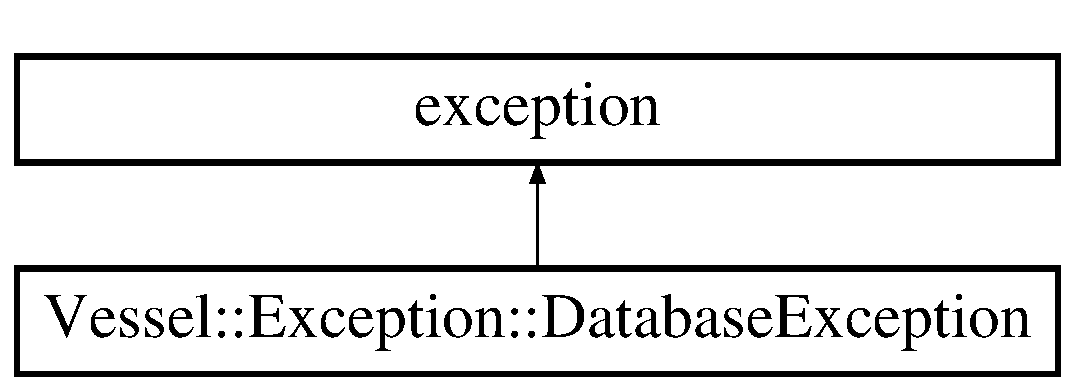
\includegraphics[height=2.000000cm]{class_vessel_1_1_exception_1_1_database_exception}
\end{center}
\end{figure}
\subsection*{Public Types}
\begin{DoxyCompactItemize}
\item 
\mbox{\Hypertarget{class_vessel_1_1_exception_1_1_database_exception_ab135bfa02ded1e5a862e2f3299128d37}\label{class_vessel_1_1_exception_1_1_database_exception_ab135bfa02ded1e5a862e2f3299128d37}} 
enum {\bfseries Error\+Code} \{ {\bfseries No\+Error} = 0, 
{\bfseries Invalid\+Query}, 
{\bfseries Invalid\+Statement}, 
{\bfseries No\+Results}
 \}
\end{DoxyCompactItemize}
\subsection*{Public Member Functions}
\begin{DoxyCompactItemize}
\item 
\mbox{\Hypertarget{class_vessel_1_1_exception_1_1_database_exception_ac9328d758ce098b81a744bab973eb945}\label{class_vessel_1_1_exception_1_1_database_exception_ac9328d758ce098b81a744bab973eb945}} 
{\bfseries Database\+Exception} (Error\+Code e, const std\+::string \&msg)
\item 
\mbox{\Hypertarget{class_vessel_1_1_exception_1_1_database_exception_ab38886bc94c9d0e00dc932601db7a1f1}\label{class_vessel_1_1_exception_1_1_database_exception_ab38886bc94c9d0e00dc932601db7a1f1}} 
Error\+Code {\bfseries get\+\_\+code} ()
\item 
\mbox{\Hypertarget{class_vessel_1_1_exception_1_1_database_exception_ad9102ff132bec42ebd89117178bd6614}\label{class_vessel_1_1_exception_1_1_database_exception_ad9102ff132bec42ebd89117178bd6614}} 
virtual const char $\ast$ {\bfseries what} () const noexcept override
\end{DoxyCompactItemize}


The documentation for this class was generated from the following file\+:\begin{DoxyCompactItemize}
\item 
/home/kyle/cpp/bv-\/backup/include/vessel/database/db\+\_\+exception.\+hpp\end{DoxyCompactItemize}

\hypertarget{struct_vessel_1_1_types_1_1file__directory}{}\section{Vessel\+:\+:Types\+:\+:file\+\_\+directory Struct Reference}
\label{struct_vessel_1_1_types_1_1file__directory}\index{Vessel\+::\+Types\+::file\+\_\+directory@{Vessel\+::\+Types\+::file\+\_\+directory}}
\subsection*{Public Attributes}
\begin{DoxyCompactItemize}
\item 
\mbox{\Hypertarget{struct_vessel_1_1_types_1_1file__directory_a2b0d8994875f5e09536cfe986684aca0}\label{struct_vessel_1_1_types_1_1file__directory_a2b0d8994875f5e09536cfe986684aca0}} 
std\+::string {\bfseries folder\+\_\+name}
\item 
\mbox{\Hypertarget{struct_vessel_1_1_types_1_1file__directory_abd82ff6f74b07186963817ee763ea9c7}\label{struct_vessel_1_1_types_1_1file__directory_abd82ff6f74b07186963817ee763ea9c7}} 
std\+::string {\bfseries path}
\item 
\mbox{\Hypertarget{struct_vessel_1_1_types_1_1file__directory_a6502484d22e9568c3022e315360eb22e}\label{struct_vessel_1_1_types_1_1file__directory_a6502484d22e9568c3022e315360eb22e}} 
unsigned int {\bfseries directory\+\_\+id}
\item 
\mbox{\Hypertarget{struct_vessel_1_1_types_1_1file__directory_aa480112ba8437fc695ce9847e7a4121c}\label{struct_vessel_1_1_types_1_1file__directory_aa480112ba8437fc695ce9847e7a4121c}} 
unsigned long {\bfseries last\+\_\+modified}
\item 
\mbox{\Hypertarget{struct_vessel_1_1_types_1_1file__directory_aa7e79295711fca3acc231fd112b39a6e}\label{struct_vessel_1_1_types_1_1file__directory_aa7e79295711fca3acc231fd112b39a6e}} 
size\+\_\+t {\bfseries filesize}
\end{DoxyCompactItemize}


The documentation for this struct was generated from the following file\+:\begin{DoxyCompactItemize}
\item 
/home/kyle/cpp/bv-\/backup/include/vessel/types.\+hpp\end{DoxyCompactItemize}

\hypertarget{class_vessel_1_1_exception_1_1_file_exception}{}\section{Vessel\+:\+:Exception\+:\+:File\+Exception Class Reference}
\label{class_vessel_1_1_exception_1_1_file_exception}\index{Vessel\+::\+Exception\+::\+File\+Exception@{Vessel\+::\+Exception\+::\+File\+Exception}}
Inheritance diagram for Vessel\+:\+:Exception\+:\+:File\+Exception\+:\begin{figure}[H]
\begin{center}
\leavevmode
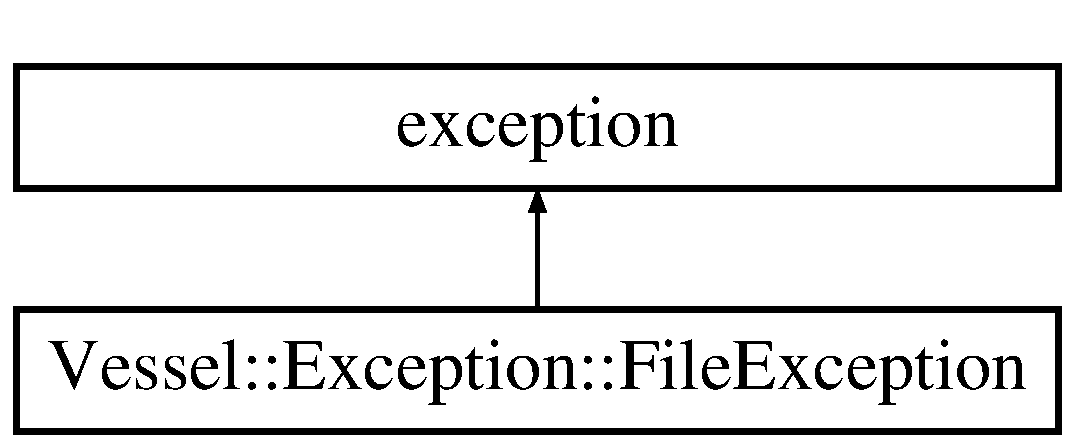
\includegraphics[height=2.000000cm]{class_vessel_1_1_exception_1_1_file_exception}
\end{center}
\end{figure}
\subsection*{Public Types}
\begin{DoxyCompactItemize}
\item 
\mbox{\Hypertarget{class_vessel_1_1_exception_1_1_file_exception_acfaea4e62709b3af50193eda37ef4b80}\label{class_vessel_1_1_exception_1_1_file_exception_acfaea4e62709b3af50193eda37ef4b80}} 
enum {\bfseries Error\+Code} \{ {\bfseries No\+Error} = 0, 
{\bfseries File\+Not\+Found}, 
{\bfseries Read\+Error}, 
{\bfseries Dir\+Not\+Found}
 \}
\end{DoxyCompactItemize}
\subsection*{Public Member Functions}
\begin{DoxyCompactItemize}
\item 
\mbox{\Hypertarget{class_vessel_1_1_exception_1_1_file_exception_a32d77bd0b49d0601a701e223025f9d51}\label{class_vessel_1_1_exception_1_1_file_exception_a32d77bd0b49d0601a701e223025f9d51}} 
{\bfseries File\+Exception} (Error\+Code e, const std\+::string \&msg)
\item 
\mbox{\Hypertarget{class_vessel_1_1_exception_1_1_file_exception_af1de58f302b25400e03dea37111a9296}\label{class_vessel_1_1_exception_1_1_file_exception_af1de58f302b25400e03dea37111a9296}} 
Error\+Code {\bfseries get\+\_\+code} ()
\item 
\mbox{\Hypertarget{class_vessel_1_1_exception_1_1_file_exception_adc6d029a67b9c5c5ab89697f51894650}\label{class_vessel_1_1_exception_1_1_file_exception_adc6d029a67b9c5c5ab89697f51894650}} 
virtual const char $\ast$ {\bfseries what} () const noexcept override
\end{DoxyCompactItemize}


The documentation for this class was generated from the following file\+:\begin{DoxyCompactItemize}
\item 
/home/kyle/cpp/bv-\/backup/include/vessel/filesystem/file\+\_\+exception.\+hpp\end{DoxyCompactItemize}

\hypertarget{class_vessel_1_1_file_1_1_file_iterator}{}\section{Vessel\+:\+:File\+:\+:File\+Iterator Class Reference}
\label{class_vessel_1_1_file_1_1_file_iterator}\index{Vessel\+::\+File\+::\+File\+Iterator@{Vessel\+::\+File\+::\+File\+Iterator}}


Helper class for scanning files and adding them to the database.  




{\ttfamily \#include $<$file\+\_\+iterator.\+hpp$>$}

\subsection*{Public Member Functions}
\begin{DoxyCompactItemize}
\item 
\mbox{\Hypertarget{class_vessel_1_1_file_1_1_file_iterator_a0607caa735b9d506bfa7dcdc635416a2}\label{class_vessel_1_1_file_1_1_file_iterator_a0607caa735b9d506bfa7dcdc635416a2}} 
{\bfseries File\+Iterator} (const \hyperlink{class_vessel_1_1_file_1_1_backup_directory}{Backup\+Directory} \&bd)
\item 
\mbox{\Hypertarget{class_vessel_1_1_file_1_1_file_iterator_a23c4a395200a4a77abacd716fed5cb14}\label{class_vessel_1_1_file_1_1_file_iterator_a23c4a395200a4a77abacd716fed5cb14}} 
void \hyperlink{class_vessel_1_1_file_1_1_file_iterator_a23c4a395200a4a77abacd716fed5cb14}{scan} ()
\begin{DoxyCompactList}\small\item\em Scans the filesystem for files and directories. \end{DoxyCompactList}\item 
std\+::string \hyperlink{class_vessel_1_1_file_1_1_file_iterator_a8701998833ac62c2618d815fc100f6d1}{get\+\_\+base\+\_\+path} ()
\begin{DoxyCompactList}\small\item\em Returns the default scan path for the current user. \end{DoxyCompactList}\item 
bool \hyperlink{class_vessel_1_1_file_1_1_file_iterator_aed179f0336b6955a56fc97905404faef}{is\+\_\+ignore\+\_\+dir} (const boost\+::filesystem\+::path \&p, int level)
\begin{DoxyCompactList}\small\item\em Checks if the directory is being ignored. \end{DoxyCompactList}\item 
bool \hyperlink{class_vessel_1_1_file_1_1_file_iterator_a6f285e42ac14fcb265d72299131b1ffe}{is\+\_\+ignore\+\_\+ext} (const std\+::string \&ext)
\begin{DoxyCompactList}\small\item\em Checks if the file extension is ignored. \end{DoxyCompactList}\item 
bool \hyperlink{class_vessel_1_1_file_1_1_file_iterator_a89f4f4d25b18640d3201c558d56cbb5d}{add\+\_\+file} (const \hyperlink{class_vessel_1_1_file_1_1_backup_file}{Backup\+File} \&bf)
\begin{DoxyCompactList}\small\item\em Adds a file to the database. \end{DoxyCompactList}\item 
int \hyperlink{class_vessel_1_1_file_1_1_file_iterator_a131ad68618d2f9d649ca28cf5fa923f5}{add\+\_\+directory} (const \hyperlink{class_vessel_1_1_file_1_1_backup_directory}{Backup\+Directory} \&bd)
\begin{DoxyCompactList}\small\item\em Adds a directory to the database. \end{DoxyCompactList}\end{DoxyCompactItemize}


\subsection{Detailed Description}
Helper class for scanning files and adding them to the database. 

\subsection{Member Function Documentation}
\mbox{\Hypertarget{class_vessel_1_1_file_1_1_file_iterator_a131ad68618d2f9d649ca28cf5fa923f5}\label{class_vessel_1_1_file_1_1_file_iterator_a131ad68618d2f9d649ca28cf5fa923f5}} 
\index{Vessel\+::\+File\+::\+File\+Iterator@{Vessel\+::\+File\+::\+File\+Iterator}!add\+\_\+directory@{add\+\_\+directory}}
\index{add\+\_\+directory@{add\+\_\+directory}!Vessel\+::\+File\+::\+File\+Iterator@{Vessel\+::\+File\+::\+File\+Iterator}}
\subsubsection{\texorpdfstring{add\+\_\+directory()}{add\_directory()}}
{\footnotesize\ttfamily int Vessel\+::\+File\+::\+File\+Iterator\+::add\+\_\+directory (\begin{DoxyParamCaption}\item[{const \hyperlink{class_vessel_1_1_file_1_1_backup_directory}{Backup\+Directory} \&}]{bd }\end{DoxyParamCaption})}



Adds a directory to the database. 

\begin{DoxyReturn}{Returns}
Returns the database directory id (integer) or -\/1 if the operation fails 
\end{DoxyReturn}
\mbox{\Hypertarget{class_vessel_1_1_file_1_1_file_iterator_a89f4f4d25b18640d3201c558d56cbb5d}\label{class_vessel_1_1_file_1_1_file_iterator_a89f4f4d25b18640d3201c558d56cbb5d}} 
\index{Vessel\+::\+File\+::\+File\+Iterator@{Vessel\+::\+File\+::\+File\+Iterator}!add\+\_\+file@{add\+\_\+file}}
\index{add\+\_\+file@{add\+\_\+file}!Vessel\+::\+File\+::\+File\+Iterator@{Vessel\+::\+File\+::\+File\+Iterator}}
\subsubsection{\texorpdfstring{add\+\_\+file()}{add\_file()}}
{\footnotesize\ttfamily int Vessel\+::\+File\+::\+File\+Iterator\+::add\+\_\+file (\begin{DoxyParamCaption}\item[{const \hyperlink{class_vessel_1_1_file_1_1_backup_file}{Backup\+File} \&}]{bf }\end{DoxyParamCaption})}



Adds a file to the database. 

\begin{DoxyReturn}{Returns}
Returns true if the file extension is ignored 
\end{DoxyReturn}
\mbox{\Hypertarget{class_vessel_1_1_file_1_1_file_iterator_a8701998833ac62c2618d815fc100f6d1}\label{class_vessel_1_1_file_1_1_file_iterator_a8701998833ac62c2618d815fc100f6d1}} 
\index{Vessel\+::\+File\+::\+File\+Iterator@{Vessel\+::\+File\+::\+File\+Iterator}!get\+\_\+base\+\_\+path@{get\+\_\+base\+\_\+path}}
\index{get\+\_\+base\+\_\+path@{get\+\_\+base\+\_\+path}!Vessel\+::\+File\+::\+File\+Iterator@{Vessel\+::\+File\+::\+File\+Iterator}}
\subsubsection{\texorpdfstring{get\+\_\+base\+\_\+path()}{get\_base\_path()}}
{\footnotesize\ttfamily std\+::string Vessel\+::\+File\+::\+File\+Iterator\+::get\+\_\+base\+\_\+path (\begin{DoxyParamCaption}{ }\end{DoxyParamCaption})}



Returns the default scan path for the current user. 

\begin{DoxyReturn}{Returns}
Returns the default scan path for the current user 
\end{DoxyReturn}
\mbox{\Hypertarget{class_vessel_1_1_file_1_1_file_iterator_aed179f0336b6955a56fc97905404faef}\label{class_vessel_1_1_file_1_1_file_iterator_aed179f0336b6955a56fc97905404faef}} 
\index{Vessel\+::\+File\+::\+File\+Iterator@{Vessel\+::\+File\+::\+File\+Iterator}!is\+\_\+ignore\+\_\+dir@{is\+\_\+ignore\+\_\+dir}}
\index{is\+\_\+ignore\+\_\+dir@{is\+\_\+ignore\+\_\+dir}!Vessel\+::\+File\+::\+File\+Iterator@{Vessel\+::\+File\+::\+File\+Iterator}}
\subsubsection{\texorpdfstring{is\+\_\+ignore\+\_\+dir()}{is\_ignore\_dir()}}
{\footnotesize\ttfamily bool Vessel\+::\+File\+::\+File\+Iterator\+::is\+\_\+ignore\+\_\+dir (\begin{DoxyParamCaption}\item[{const boost\+::filesystem\+::path \&}]{p,  }\item[{int}]{level }\end{DoxyParamCaption})}



Checks if the directory is being ignored. 


\begin{DoxyParams}{Parameters}
{\em level} & Enforces the nesting level of the directory \\
\hline
\end{DoxyParams}
\begin{DoxyReturn}{Returns}
Returns true if the directory is being ignored 
\end{DoxyReturn}
\mbox{\Hypertarget{class_vessel_1_1_file_1_1_file_iterator_a6f285e42ac14fcb265d72299131b1ffe}\label{class_vessel_1_1_file_1_1_file_iterator_a6f285e42ac14fcb265d72299131b1ffe}} 
\index{Vessel\+::\+File\+::\+File\+Iterator@{Vessel\+::\+File\+::\+File\+Iterator}!is\+\_\+ignore\+\_\+ext@{is\+\_\+ignore\+\_\+ext}}
\index{is\+\_\+ignore\+\_\+ext@{is\+\_\+ignore\+\_\+ext}!Vessel\+::\+File\+::\+File\+Iterator@{Vessel\+::\+File\+::\+File\+Iterator}}
\subsubsection{\texorpdfstring{is\+\_\+ignore\+\_\+ext()}{is\_ignore\_ext()}}
{\footnotesize\ttfamily bool Vessel\+::\+File\+::\+File\+Iterator\+::is\+\_\+ignore\+\_\+ext (\begin{DoxyParamCaption}\item[{const std\+::string \&}]{ext }\end{DoxyParamCaption})}



Checks if the file extension is ignored. 


\begin{DoxyParams}{Parameters}
{\em ext} & The file extension (eg. .jpg) \\
\hline
\end{DoxyParams}
\begin{DoxyReturn}{Returns}
Returns true if the file extension is ignored 
\end{DoxyReturn}


The documentation for this class was generated from the following file\+:\begin{DoxyCompactItemize}
\item 
/home/kyle/cpp/bv-\/backup/include/vessel/filesystem/file\+\_\+iterator.\+hpp\end{DoxyCompactItemize}

\hypertarget{struct_vessel_1_1_types_1_1_file_part}{}\section{Vessel\+:\+:Types\+:\+:File\+Part Struct Reference}
\label{struct_vessel_1_1_types_1_1_file_part}\index{Vessel\+::\+Types\+::\+File\+Part@{Vessel\+::\+Types\+::\+File\+Part}}
\subsection*{Public Attributes}
\begin{DoxyCompactItemize}
\item 
\mbox{\Hypertarget{struct_vessel_1_1_types_1_1_file_part_afd739fe0596eec0e6f42a46678f6b67d}\label{struct_vessel_1_1_types_1_1_file_part_afd739fe0596eec0e6f42a46678f6b67d}} 
unsigned int {\bfseries upload\+\_\+id}
\item 
\mbox{\Hypertarget{struct_vessel_1_1_types_1_1_file_part_a99193b637fe6c86582b7f39142090de1}\label{struct_vessel_1_1_types_1_1_file_part_a99193b637fe6c86582b7f39142090de1}} 
std\+::string {\bfseries upload\+\_\+key}
\item 
\mbox{\Hypertarget{struct_vessel_1_1_types_1_1_file_part_a27ef31c339bd6195a1ea3f5137f600b4}\label{struct_vessel_1_1_types_1_1_file_part_a27ef31c339bd6195a1ea3f5137f600b4}} 
int {\bfseries part\+\_\+number}
\item 
\mbox{\Hypertarget{struct_vessel_1_1_types_1_1_file_part_a830f548fb98c9dd10e1e8bf92149d974}\label{struct_vessel_1_1_types_1_1_file_part_a830f548fb98c9dd10e1e8bf92149d974}} 
size\+\_\+t {\bfseries total\+\_\+bytes}
\item 
\mbox{\Hypertarget{struct_vessel_1_1_types_1_1_file_part_ad6e9dc2a3bf167ff5cbce4b6328b1bf9}\label{struct_vessel_1_1_types_1_1_file_part_ad6e9dc2a3bf167ff5cbce4b6328b1bf9}} 
std\+::string {\bfseries tag}
\item 
\mbox{\Hypertarget{struct_vessel_1_1_types_1_1_file_part_ab317c93b6922952bcc834179e5df7f6f}\label{struct_vessel_1_1_types_1_1_file_part_ab317c93b6922952bcc834179e5df7f6f}} 
std\+::string {\bfseries signature}
\end{DoxyCompactItemize}


The documentation for this struct was generated from the following file\+:\begin{DoxyCompactItemize}
\item 
/home/kyle/cpp/bv-\/backup/include/vessel/types.\+hpp\end{DoxyCompactItemize}

\hypertarget{class_vessel_1_1_file_1_1_file_upload}{}\section{Vessel\+:\+:File\+:\+:File\+Upload Class Reference}
\label{class_vessel_1_1_file_1_1_file_upload}\index{Vessel\+::\+File\+::\+File\+Upload@{Vessel\+::\+File\+::\+File\+Upload}}
\subsection*{Public Member Functions}
\begin{DoxyCompactItemize}
\item 
\mbox{\Hypertarget{class_vessel_1_1_file_1_1_file_upload_ae4cf17d031fc2ef3c40ef7169181f8f3}\label{class_vessel_1_1_file_1_1_file_upload_ae4cf17d031fc2ef3c40ef7169181f8f3}} 
{\bfseries File\+Upload} (const std\+::string \&upload\+\_\+key)
\item 
\mbox{\Hypertarget{class_vessel_1_1_file_1_1_file_upload_a2356608e1bf014feba93dba394f4e9ee}\label{class_vessel_1_1_file_1_1_file_upload_a2356608e1bf014feba93dba394f4e9ee}} 
{\bfseries File\+Upload} (unsigned int upload\+\_\+id)
\item 
\mbox{\Hypertarget{class_vessel_1_1_file_1_1_file_upload_a2b6613dbefe6cef42e7a90d85ff42be6}\label{class_vessel_1_1_file_1_1_file_upload_a2b6613dbefe6cef42e7a90d85ff42be6}} 
unsigned int {\bfseries get\+\_\+upload\+\_\+id} () const
\item 
\mbox{\Hypertarget{class_vessel_1_1_file_1_1_file_upload_afcffcd79f065514b1306da4e3ccdae0c}\label{class_vessel_1_1_file_1_1_file_upload_afcffcd79f065514b1306da4e3ccdae0c}} 
std\+::string {\bfseries get\+\_\+upload\+\_\+key} () const
\item 
\mbox{\Hypertarget{class_vessel_1_1_file_1_1_file_upload_a1aea0a2c881b55dc6800d7e2a61cb6dd}\label{class_vessel_1_1_file_1_1_file_upload_a1aea0a2c881b55dc6800d7e2a61cb6dd}} 
std\+::string {\bfseries get\+\_\+hash} () const
\item 
\mbox{\Hypertarget{class_vessel_1_1_file_1_1_file_upload_a7368ab66aa36b85d6e8b1c5dc6c89b16}\label{class_vessel_1_1_file_1_1_file_upload_a7368ab66aa36b85d6e8b1c5dc6c89b16}} 
std\+::string {\bfseries get\+\_\+signature} () const
\item 
\mbox{\Hypertarget{class_vessel_1_1_file_1_1_file_upload_ae5a9c73d0a1cfe50c11889f6390c53ca}\label{class_vessel_1_1_file_1_1_file_upload_ae5a9c73d0a1cfe50c11889f6390c53ca}} 
int {\bfseries get\+\_\+total\+\_\+parts} () const
\item 
\mbox{\Hypertarget{class_vessel_1_1_file_1_1_file_upload_a633667ce1140e8586be898fe8b9bc7b0}\label{class_vessel_1_1_file_1_1_file_upload_a633667ce1140e8586be898fe8b9bc7b0}} 
int {\bfseries get\+\_\+offset} () const
\item 
\mbox{\Hypertarget{class_vessel_1_1_file_1_1_file_upload_ad5f531dbb198fb66b96dd3c12ec32d6e}\label{class_vessel_1_1_file_1_1_file_upload_ad5f531dbb198fb66b96dd3c12ec32d6e}} 
int {\bfseries get\+\_\+weight} () const
\item 
\mbox{\Hypertarget{class_vessel_1_1_file_1_1_file_upload_ac88dd9961a6f6c97a225aac7078a3d2e}\label{class_vessel_1_1_file_1_1_file_upload_ac88dd9961a6f6c97a225aac7078a3d2e}} 
unsigned int {\bfseries get\+\_\+chunk\+\_\+size} () const
\item 
\mbox{\Hypertarget{class_vessel_1_1_file_1_1_file_upload_a0c25202d895a62d71371d15a6f2df3fc}\label{class_vessel_1_1_file_1_1_file_upload_a0c25202d895a62d71371d15a6f2df3fc}} 
unsigned long {\bfseries get\+\_\+last\+\_\+modified} () const
\item 
\mbox{\Hypertarget{class_vessel_1_1_file_1_1_file_upload_aa45a65f551eb4a784946300ad46bcc34}\label{class_vessel_1_1_file_1_1_file_upload_aa45a65f551eb4a784946300ad46bcc34}} 
bool {\bfseries exists} () const
\item 
\mbox{\Hypertarget{class_vessel_1_1_file_1_1_file_upload_a1f76a234eb2b64bb851ae6c27b45507f}\label{class_vessel_1_1_file_1_1_file_upload_a1f76a234eb2b64bb851ae6c27b45507f}} 
\hyperlink{class_vessel_1_1_file_1_1_backup_file}{Backup\+File} {\bfseries get\+\_\+file} ()
\item 
\mbox{\Hypertarget{class_vessel_1_1_file_1_1_file_upload_a342107a641cc851054048c9a0e78c5a9}\label{class_vessel_1_1_file_1_1_file_upload_a342107a641cc851054048c9a0e78c5a9}} 
std\+::shared\+\_\+ptr$<$ unsigned char $>$ {\bfseries get\+\_\+file\+\_\+id} ()
\item 
\mbox{\Hypertarget{class_vessel_1_1_file_1_1_file_upload_a1fb93cce7e2f84cda20b219c131bb2c8}\label{class_vessel_1_1_file_1_1_file_upload_a1fb93cce7e2f84cda20b219c131bb2c8}} 
void {\bfseries update\+\_\+key} (const std\+::string \&upload\+\_\+key)
\item 
\mbox{\Hypertarget{class_vessel_1_1_file_1_1_file_upload_ad832f96cdbffe0410b353c3835f19f78}\label{class_vessel_1_1_file_1_1_file_upload_ad832f96cdbffe0410b353c3835f19f78}} 
int {\bfseries get\+\_\+current\+\_\+part} () const
\item 
\mbox{\Hypertarget{class_vessel_1_1_file_1_1_file_upload_ae477b17b940ab1c86b8dae8780c08206}\label{class_vessel_1_1_file_1_1_file_upload_ae477b17b940ab1c86b8dae8780c08206}} 
void {\bfseries add\+\_\+part} (const \hyperlink{struct_vessel_1_1_types_1_1_file_part}{File\+Part} \&part) const
\item 
\mbox{\Hypertarget{class_vessel_1_1_file_1_1_file_upload_a9bb4ff3bb9b28a506a2907ddd7373a08}\label{class_vessel_1_1_file_1_1_file_upload_a9bb4ff3bb9b28a506a2907ddd7373a08}} 
std\+::vector$<$ \hyperlink{struct_vessel_1_1_types_1_1_upload_tag_set}{Upload\+Tag\+Set} $>$ {\bfseries get\+\_\+part\+\_\+tags} () const
\item 
\mbox{\Hypertarget{class_vessel_1_1_file_1_1_file_upload_a2fd38aef6fbc243aa677e4f74bb70168}\label{class_vessel_1_1_file_1_1_file_upload_a2fd38aef6fbc243aa677e4f74bb70168}} 
int {\bfseries get\+\_\+error\+\_\+count} () const
\item 
\mbox{\Hypertarget{class_vessel_1_1_file_1_1_file_upload_ae86a8cab440ab34b762232227c27ed68}\label{class_vessel_1_1_file_1_1_file_upload_ae86a8cab440ab34b762232227c27ed68}} 
int {\bfseries increment\+\_\+error} ()
\end{DoxyCompactItemize}


The documentation for this class was generated from the following file\+:\begin{DoxyCompactItemize}
\item 
/home/kyle/cpp/bv-\/backup/include/vessel/filesystem/file\+\_\+upload.\+hpp\end{DoxyCompactItemize}

\hypertarget{class_vessel_1_1_utilities_1_1_hash}{}\section{Vessel\+:\+:Utilities\+:\+:Hash Class Reference}
\label{class_vessel_1_1_utilities_1_1_hash}\index{Vessel\+::\+Utilities\+::\+Hash@{Vessel\+::\+Utilities\+::\+Hash}}
\subsection*{Static Public Member Functions}
\begin{DoxyCompactItemize}
\item 
static std\+::shared\+\_\+ptr$<$ unsigned char $>$ \hyperlink{class_vessel_1_1_utilities_1_1_hash_aae24b1d2642ec244551857894a13f533}{get\+\_\+sha1\+\_\+hash\+\_\+ptr} (const std\+::string \&data)
\begin{DoxyCompactList}\small\item\em Returns a shared\+\_\+ptr to a binary id (unsigned char$\ast$) \end{DoxyCompactList}\item 
static std\+::string \hyperlink{class_vessel_1_1_utilities_1_1_hash_aac0daddfa7414c8e9ee27c1f4b811e6c}{get\+\_\+sha1\+\_\+hash} (const std\+::string \&data)
\begin{DoxyCompactList}\small\item\em Returns a sha-\/1 hash string. \end{DoxyCompactList}\item 
static std\+::string \hyperlink{class_vessel_1_1_utilities_1_1_hash_ac2947d4601160bd693f94fbb03a567c2}{get\+\_\+sha256\+\_\+hash} (const std\+::string \&data)
\begin{DoxyCompactList}\small\item\em Returns a sha-\/256 hash string. \end{DoxyCompactList}\item 
static std\+::string \hyperlink{class_vessel_1_1_utilities_1_1_hash_a453b9f3c511af3c444b8aca245ee9405}{get\+\_\+md5\+\_\+hash} (const std\+::string \&data, bool base64=false)
\begin{DoxyCompactList}\small\item\em Returns a md5 hash string. \end{DoxyCompactList}\item 
static std\+::string \hyperlink{class_vessel_1_1_utilities_1_1_hash_ae618a6d2856efcf77399aab0dc8d7848}{get\+\_\+base64} (const std\+::string \&data)
\begin{DoxyCompactList}\small\item\em Returns a base64 encoded string. \end{DoxyCompactList}\item 
static std\+::string \hyperlink{class_vessel_1_1_utilities_1_1_hash_af263070a887f314a5ea27316258a87ac}{get\+\_\+hmac\+\_\+256} (const std\+::string \&key, const std\+::string \&data, bool hex=true)
\begin{DoxyCompactList}\small\item\em Returns a H\+M\+AC S\+H\+A-\/256 string. \end{DoxyCompactList}\item 
static std\+::string \hyperlink{class_vessel_1_1_utilities_1_1_hash_a0e1b698d8ab1aea9f1d7a47789e055ea}{base64\+\_\+decode} (const std\+::string \&str)
\begin{DoxyCompactList}\small\item\em Returns a base64 decoded string. \end{DoxyCompactList}\end{DoxyCompactItemize}


\subsection{Detailed Description}
class for common crypto style functions 

\subsection{Member Function Documentation}
\mbox{\Hypertarget{class_vessel_1_1_utilities_1_1_hash_a0e1b698d8ab1aea9f1d7a47789e055ea}\label{class_vessel_1_1_utilities_1_1_hash_a0e1b698d8ab1aea9f1d7a47789e055ea}} 
\index{Vessel\+::\+Utilities\+::\+Hash@{Vessel\+::\+Utilities\+::\+Hash}!base64\+\_\+decode@{base64\+\_\+decode}}
\index{base64\+\_\+decode@{base64\+\_\+decode}!Vessel\+::\+Utilities\+::\+Hash@{Vessel\+::\+Utilities\+::\+Hash}}
\subsubsection{\texorpdfstring{base64\+\_\+decode()}{base64\_decode()}}
{\footnotesize\ttfamily static std\+::string Vessel\+::\+Utilities\+::\+Hash\+::base64\+\_\+decode (\begin{DoxyParamCaption}\item[{const std\+::string \&}]{str }\end{DoxyParamCaption})\hspace{0.3cm}{\ttfamily [static]}}



Returns a base64 decoded string. 


\begin{DoxyParams}{Parameters}
{\em str} & Base64 encoded string to decode \\
\hline
\end{DoxyParams}
\begin{DoxyReturn}{Returns}
Returns a base64 decoded string 
\end{DoxyReturn}
\mbox{\Hypertarget{class_vessel_1_1_utilities_1_1_hash_ae618a6d2856efcf77399aab0dc8d7848}\label{class_vessel_1_1_utilities_1_1_hash_ae618a6d2856efcf77399aab0dc8d7848}} 
\index{Vessel\+::\+Utilities\+::\+Hash@{Vessel\+::\+Utilities\+::\+Hash}!get\+\_\+base64@{get\+\_\+base64}}
\index{get\+\_\+base64@{get\+\_\+base64}!Vessel\+::\+Utilities\+::\+Hash@{Vessel\+::\+Utilities\+::\+Hash}}
\subsubsection{\texorpdfstring{get\+\_\+base64()}{get\_base64()}}
{\footnotesize\ttfamily static std\+::string Vessel\+::\+Utilities\+::\+Hash\+::get\+\_\+base64 (\begin{DoxyParamCaption}\item[{const std\+::string \&}]{data }\end{DoxyParamCaption})\hspace{0.3cm}{\ttfamily [static]}}



Returns a base64 encoded string. 

\begin{DoxyReturn}{Returns}
Returns a base64 encoded string 
\end{DoxyReturn}
\mbox{\Hypertarget{class_vessel_1_1_utilities_1_1_hash_af263070a887f314a5ea27316258a87ac}\label{class_vessel_1_1_utilities_1_1_hash_af263070a887f314a5ea27316258a87ac}} 
\index{Vessel\+::\+Utilities\+::\+Hash@{Vessel\+::\+Utilities\+::\+Hash}!get\+\_\+hmac\+\_\+256@{get\+\_\+hmac\+\_\+256}}
\index{get\+\_\+hmac\+\_\+256@{get\+\_\+hmac\+\_\+256}!Vessel\+::\+Utilities\+::\+Hash@{Vessel\+::\+Utilities\+::\+Hash}}
\subsubsection{\texorpdfstring{get\+\_\+hmac\+\_\+256()}{get\_hmac\_256()}}
{\footnotesize\ttfamily static std\+::string Vessel\+::\+Utilities\+::\+Hash\+::get\+\_\+hmac\+\_\+256 (\begin{DoxyParamCaption}\item[{const std\+::string \&}]{key,  }\item[{const std\+::string \&}]{data,  }\item[{bool}]{hex = {\ttfamily true} }\end{DoxyParamCaption})\hspace{0.3cm}{\ttfamily [static]}}



Returns a H\+M\+AC S\+H\+A-\/256 string. 


\begin{DoxyParams}{Parameters}
{\em key} & Key string used to generate the H\+M\+AC \\
\hline
{\em data} & Data to be used when calculating the H\+M\+AC \\
\hline
{\em hex} & Hex encodes the string if set to true \\
\hline
\end{DoxyParams}
\begin{DoxyReturn}{Returns}
Returns a H\+M\+AC S\+H\+A-\/256 string 
\end{DoxyReturn}
\mbox{\Hypertarget{class_vessel_1_1_utilities_1_1_hash_a453b9f3c511af3c444b8aca245ee9405}\label{class_vessel_1_1_utilities_1_1_hash_a453b9f3c511af3c444b8aca245ee9405}} 
\index{Vessel\+::\+Utilities\+::\+Hash@{Vessel\+::\+Utilities\+::\+Hash}!get\+\_\+md5\+\_\+hash@{get\+\_\+md5\+\_\+hash}}
\index{get\+\_\+md5\+\_\+hash@{get\+\_\+md5\+\_\+hash}!Vessel\+::\+Utilities\+::\+Hash@{Vessel\+::\+Utilities\+::\+Hash}}
\subsubsection{\texorpdfstring{get\+\_\+md5\+\_\+hash()}{get\_md5\_hash()}}
{\footnotesize\ttfamily static std\+::string Vessel\+::\+Utilities\+::\+Hash\+::get\+\_\+md5\+\_\+hash (\begin{DoxyParamCaption}\item[{const std\+::string \&}]{data,  }\item[{bool}]{base64 = {\ttfamily false} }\end{DoxyParamCaption})\hspace{0.3cm}{\ttfamily [static]}}



Returns a md5 hash string. 


\begin{DoxyParams}{Parameters}
{\em base64} & Base64 encodes the string if set to true \\
\hline
\end{DoxyParams}
\begin{DoxyReturn}{Returns}
Returns a md5 hash string 
\end{DoxyReturn}
\mbox{\Hypertarget{class_vessel_1_1_utilities_1_1_hash_aac0daddfa7414c8e9ee27c1f4b811e6c}\label{class_vessel_1_1_utilities_1_1_hash_aac0daddfa7414c8e9ee27c1f4b811e6c}} 
\index{Vessel\+::\+Utilities\+::\+Hash@{Vessel\+::\+Utilities\+::\+Hash}!get\+\_\+sha1\+\_\+hash@{get\+\_\+sha1\+\_\+hash}}
\index{get\+\_\+sha1\+\_\+hash@{get\+\_\+sha1\+\_\+hash}!Vessel\+::\+Utilities\+::\+Hash@{Vessel\+::\+Utilities\+::\+Hash}}
\subsubsection{\texorpdfstring{get\+\_\+sha1\+\_\+hash()}{get\_sha1\_hash()}}
{\footnotesize\ttfamily static std\+::string Vessel\+::\+Utilities\+::\+Hash\+::get\+\_\+sha1\+\_\+hash (\begin{DoxyParamCaption}\item[{const std\+::string \&}]{data }\end{DoxyParamCaption})\hspace{0.3cm}{\ttfamily [static]}}



Returns a sha-\/1 hash string. 

\begin{DoxyReturn}{Returns}
Returns a sha-\/1 hash string 
\end{DoxyReturn}
\mbox{\Hypertarget{class_vessel_1_1_utilities_1_1_hash_aae24b1d2642ec244551857894a13f533}\label{class_vessel_1_1_utilities_1_1_hash_aae24b1d2642ec244551857894a13f533}} 
\index{Vessel\+::\+Utilities\+::\+Hash@{Vessel\+::\+Utilities\+::\+Hash}!get\+\_\+sha1\+\_\+hash\+\_\+ptr@{get\+\_\+sha1\+\_\+hash\+\_\+ptr}}
\index{get\+\_\+sha1\+\_\+hash\+\_\+ptr@{get\+\_\+sha1\+\_\+hash\+\_\+ptr}!Vessel\+::\+Utilities\+::\+Hash@{Vessel\+::\+Utilities\+::\+Hash}}
\subsubsection{\texorpdfstring{get\+\_\+sha1\+\_\+hash\+\_\+ptr()}{get\_sha1\_hash\_ptr()}}
{\footnotesize\ttfamily static std\+::shared\+\_\+ptr$<$ unsigned char $>$ Vessel\+::\+Utilities\+::\+Hash\+::get\+\_\+sha1\+\_\+hash\+\_\+ptr (\begin{DoxyParamCaption}\item[{const std\+::string \&}]{data }\end{DoxyParamCaption})\hspace{0.3cm}{\ttfamily [static]}}



Returns a shared\+\_\+ptr to a binary id (unsigned char$\ast$) 

\begin{DoxyReturn}{Returns}
Returns a shared\+\_\+ptr to a binary id (unsigned char$\ast$) 
\end{DoxyReturn}
\mbox{\Hypertarget{class_vessel_1_1_utilities_1_1_hash_ac2947d4601160bd693f94fbb03a567c2}\label{class_vessel_1_1_utilities_1_1_hash_ac2947d4601160bd693f94fbb03a567c2}} 
\index{Vessel\+::\+Utilities\+::\+Hash@{Vessel\+::\+Utilities\+::\+Hash}!get\+\_\+sha256\+\_\+hash@{get\+\_\+sha256\+\_\+hash}}
\index{get\+\_\+sha256\+\_\+hash@{get\+\_\+sha256\+\_\+hash}!Vessel\+::\+Utilities\+::\+Hash@{Vessel\+::\+Utilities\+::\+Hash}}
\subsubsection{\texorpdfstring{get\+\_\+sha256\+\_\+hash()}{get\_sha256\_hash()}}
{\footnotesize\ttfamily static std\+::string Vessel\+::\+Utilities\+::\+Hash\+::get\+\_\+sha256\+\_\+hash (\begin{DoxyParamCaption}\item[{const std\+::string \&}]{data }\end{DoxyParamCaption})\hspace{0.3cm}{\ttfamily [static]}}



Returns a sha-\/256 hash string. 

\begin{DoxyReturn}{Returns}
Returns a sha-\/256 hash string 
\end{DoxyReturn}


The documentation for this class was generated from the following file\+:\begin{DoxyCompactItemize}
\item 
/home/kyle/cpp/bv-\/backup/include/vessel/crypto/hash\+\_\+util.\+hpp\end{DoxyCompactItemize}

\hypertarget{struct_vessel_1_1_types_1_1http__request}{}\section{Vessel\+:\+:Types\+:\+:http\+\_\+request Struct Reference}
\label{struct_vessel_1_1_types_1_1http__request}\index{Vessel\+::\+Types\+::http\+\_\+request@{Vessel\+::\+Types\+::http\+\_\+request}}
\subsection*{Public Attributes}
\begin{DoxyCompactItemize}
\item 
\mbox{\Hypertarget{struct_vessel_1_1_types_1_1http__request_a6621791d5b5e6d76a645c123343cc365}\label{struct_vessel_1_1_types_1_1http__request_a6621791d5b5e6d76a645c123343cc365}} 
unsigned int {\bfseries request\+\_\+type}
\item 
\mbox{\Hypertarget{struct_vessel_1_1_types_1_1http__request_a96027bd32b4a38dbc5d03c603b250df6}\label{struct_vessel_1_1_types_1_1http__request_a96027bd32b4a38dbc5d03c603b250df6}} 
std\+::string {\bfseries uri}
\item 
\mbox{\Hypertarget{struct_vessel_1_1_types_1_1http__request_a6c15d192c5cf2345144120b8f4f88444}\label{struct_vessel_1_1_types_1_1http__request_a6c15d192c5cf2345144120b8f4f88444}} 
std\+::string {\bfseries content\+\_\+type}
\item 
\mbox{\Hypertarget{struct_vessel_1_1_types_1_1http__request_a72f4911e912df0d71f7cc887fc7031ba}\label{struct_vessel_1_1_types_1_1http__request_a72f4911e912df0d71f7cc887fc7031ba}} 
std\+::string {\bfseries data}
\item 
\mbox{\Hypertarget{struct_vessel_1_1_types_1_1http__request_ab49e812c546cf319b23c622f1cb4bb00}\label{struct_vessel_1_1_types_1_1http__request_ab49e812c546cf319b23c622f1cb4bb00}} 
std\+::string {\bfseries auth\+\_\+token}
\end{DoxyCompactItemize}


The documentation for this struct was generated from the following file\+:\begin{DoxyCompactItemize}
\item 
/home/kyle/cpp/bv-\/backup/include/vessel/types.\+hpp\end{DoxyCompactItemize}

\hypertarget{class_vessel_1_1_networking_1_1_http_client}{}\section{Vessel\+:\+:Networking\+:\+:Http\+Client Class Reference}
\label{class_vessel_1_1_networking_1_1_http_client}\index{Vessel\+::\+Networking\+::\+Http\+Client@{Vessel\+::\+Networking\+::\+Http\+Client}}
Inheritance diagram for Vessel\+:\+:Networking\+:\+:Http\+Client\+:\begin{figure}[H]
\begin{center}
\leavevmode
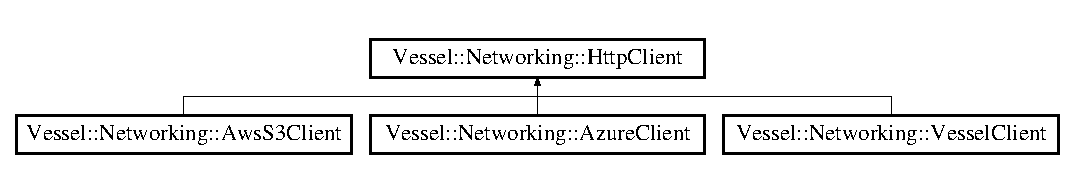
\includegraphics[height=1.830065cm]{class_vessel_1_1_networking_1_1_http_client}
\end{center}
\end{figure}
\subsection*{Public Member Functions}
\begin{DoxyCompactItemize}
\item 
\mbox{\Hypertarget{class_vessel_1_1_networking_1_1_http_client_aa71e7a5b4db62ae2a71e058145f6160e}\label{class_vessel_1_1_networking_1_1_http_client_aa71e7a5b4db62ae2a71e058145f6160e}} 
{\bfseries Http\+Client} (const std\+::string \&uri)
\item 
bool \hyperlink{class_vessel_1_1_networking_1_1_http_client_a36f814eda4b6b35e2e6991bbd0f8f672}{is\+\_\+connected} ()
\begin{DoxyCompactList}\small\item\em Return whether or not the client is currently connected. \end{DoxyCompactList}\item 
\mbox{\Hypertarget{class_vessel_1_1_networking_1_1_http_client_aa1a40ba8a7c7d6b6ff684fae7f431860}\label{class_vessel_1_1_networking_1_1_http_client_aa1a40ba8a7c7d6b6ff684fae7f431860}} 
void \hyperlink{class_vessel_1_1_networking_1_1_http_client_aa1a40ba8a7c7d6b6ff684fae7f431860}{set\+\_\+timeout} (boost\+::posix\+\_\+time\+::time\+\_\+duration t)
\begin{DoxyCompactList}\small\item\em Sets the connection timeout. \end{DoxyCompactList}\item 
\mbox{\Hypertarget{class_vessel_1_1_networking_1_1_http_client_aca87333d6add0bd783183092eaa2d552}\label{class_vessel_1_1_networking_1_1_http_client_aca87333d6add0bd783183092eaa2d552}} 
void \hyperlink{class_vessel_1_1_networking_1_1_http_client_aca87333d6add0bd783183092eaa2d552}{set\+\_\+ssl} (bool f)
\begin{DoxyCompactList}\small\item\em Set whether or not to use S\+SL when connecting. Automatically determined from U\+RL typically. \end{DoxyCompactList}\item 
std\+::string \hyperlink{class_vessel_1_1_networking_1_1_http_client_a55ce6fc94f87558d5d93f71ddbf86849}{get\+\_\+response} ()
\begin{DoxyCompactList}\small\item\em Returns the H\+T\+TP response payload. \end{DoxyCompactList}\item 
std\+::string \hyperlink{class_vessel_1_1_networking_1_1_http_client_ad5ffe2d677a1ea783a66d3ea8d57d948}{get\+\_\+headers} ()
\begin{DoxyCompactList}\small\item\em Returns the H\+T\+TP headers returned in the response. \end{DoxyCompactList}\item 
std\+::string \hyperlink{class_vessel_1_1_networking_1_1_http_client_abc244e7785648a4bd016a69f374a7e0b}{get\+\_\+header} (const std\+::string \&key)
\begin{DoxyCompactList}\small\item\em Returns the specified H\+T\+TP header value (if exists) \end{DoxyCompactList}\item 
unsigned int \hyperlink{class_vessel_1_1_networking_1_1_http_client_a0bb9af88cb6fa0cda2d613165c9a7a24}{get\+\_\+http\+\_\+status} ()
\begin{DoxyCompactList}\small\item\em Returns the H\+T\+TP status code (eg. 200) of the response. \end{DoxyCompactList}\item 
std\+::string \hyperlink{class_vessel_1_1_networking_1_1_http_client_a3038fd22cae695a56ce50aba86cad642}{get\+\_\+error} ()
\begin{DoxyCompactList}\small\item\em Returns the most recent error message recorded from the last operation. \end{DoxyCompactList}\item 
std\+::string \hyperlink{class_vessel_1_1_networking_1_1_http_client_a71876628efd404463072ea3741c5cd03}{get\+\_\+hostname} ()
\begin{DoxyCompactList}\small\item\em Returns the hostname of the U\+RI. \end{DoxyCompactList}\item 
bool \hyperlink{class_vessel_1_1_networking_1_1_http_client_ac6f264effcb5e9dc5804b3582467eb98}{is\+\_\+https} ()
\begin{DoxyCompactList}\small\item\em Returns whether or not the connection uses H\+T\+T\+PS (secure) \end{DoxyCompactList}\item 
\mbox{\Hypertarget{class_vessel_1_1_networking_1_1_http_client_a97220e27c1c9d24792d05462d64978ff}\label{class_vessel_1_1_networking_1_1_http_client_a97220e27c1c9d24792d05462d64978ff}} 
boost\+::system\+::error\+\_\+code {\bfseries get\+\_\+error\+\_\+code} ()
\item 
\mbox{\Hypertarget{class_vessel_1_1_networking_1_1_http_client_a68b254d8debf5b9dd7e5cc27fd5e60fe}\label{class_vessel_1_1_networking_1_1_http_client_a68b254d8debf5b9dd7e5cc27fd5e60fe}} 
std\+::string {\bfseries encode\+\_\+uri} (const std\+::string \&uri)
\item 
\mbox{\Hypertarget{class_vessel_1_1_networking_1_1_http_client_a42f4fc88293de8997e0ce1405db04cc5}\label{class_vessel_1_1_networking_1_1_http_client_a42f4fc88293de8997e0ce1405db04cc5}} 
std\+::string {\bfseries decode\+\_\+uri} (const std\+::string \&uri)
\item 
int \hyperlink{class_vessel_1_1_networking_1_1_http_client_a5aa9df2a1026a4aa10b6e4e51931ba04}{send\+\_\+http\+\_\+request} (const \hyperlink{class_vessel_1_1_networking_1_1_http_request}{Http\+Request} \&request)
\begin{DoxyCompactList}\small\item\em Sends a new H\+T\+TP request and writes to the socket. \end{DoxyCompactList}\item 
bool \hyperlink{class_vessel_1_1_networking_1_1_http_client_ad30f53d43a676892ac19ba2f86188ca2}{http\+\_\+logging} ()
\begin{DoxyCompactList}\small\item\em Returns true if http logging is enabled. \end{DoxyCompactList}\item 
size\+\_\+t \hyperlink{class_vessel_1_1_networking_1_1_http_client_a8c236189b1456f690a4315fa98e0d469}{get\+\_\+content\+\_\+length} ()
\begin{DoxyCompactList}\small\item\em Returns the size of the content body. \end{DoxyCompactList}\item 
int \hyperlink{class_vessel_1_1_networking_1_1_http_client_a5ad06cb85c0c5359f46df21182e908e5}{get\+\_\+port} ()
\begin{DoxyCompactList}\small\item\em Returns the port used for H\+T\+TP connection. \end{DoxyCompactList}\item 
std\+::string \hyperlink{class_vessel_1_1_networking_1_1_http_client_a3a32bbeadd12e311c4934c2841c1122d}{make\+\_\+test\+\_\+str} (size\+\_\+t length)
\begin{DoxyCompactList}\small\item\em Makes a test string of length bytes. \end{DoxyCompactList}\item 
\mbox{\Hypertarget{class_vessel_1_1_networking_1_1_http_client_a9446438a103e2690a51996c8032278c3}\label{class_vessel_1_1_networking_1_1_http_client_a9446438a103e2690a51996c8032278c3}} 
void \hyperlink{class_vessel_1_1_networking_1_1_http_client_a9446438a103e2690a51996c8032278c3}{max\+\_\+transfer\+\_\+speed} (size\+\_\+t limit)
\begin{DoxyCompactList}\small\item\em Sets the max transfer speed for H\+T\+TP requests. \end{DoxyCompactList}\end{DoxyCompactItemize}
\subsection*{Static Public Member Functions}
\begin{DoxyCompactItemize}
\item 
\mbox{\Hypertarget{class_vessel_1_1_networking_1_1_http_client_a50c01c4bbf1e2ef74caea768ad3f4401}\label{class_vessel_1_1_networking_1_1_http_client_a50c01c4bbf1e2ef74caea768ad3f4401}} 
static void \hyperlink{class_vessel_1_1_networking_1_1_http_client_a50c01c4bbf1e2ef74caea768ad3f4401}{http\+\_\+logging} (bool flag)
\begin{DoxyCompactList}\small\item\em Enables or disables H\+T\+TP logging. \end{DoxyCompactList}\end{DoxyCompactItemize}
\subsection*{Protected Member Functions}
\begin{DoxyCompactItemize}
\item 
\mbox{\Hypertarget{class_vessel_1_1_networking_1_1_http_client_a9cd9e9802dbaa9f8c2c63cb5e93b5262}\label{class_vessel_1_1_networking_1_1_http_client_a9cd9e9802dbaa9f8c2c63cb5e93b5262}} 
bool \hyperlink{class_vessel_1_1_networking_1_1_http_client_a9cd9e9802dbaa9f8c2c63cb5e93b5262}{connect} ()
\begin{DoxyCompactList}\small\item\em Connect to the master server. \end{DoxyCompactList}\item 
\mbox{\Hypertarget{class_vessel_1_1_networking_1_1_http_client_aef341ffac0b8a90420255f22edf38766}\label{class_vessel_1_1_networking_1_1_http_client_aef341ffac0b8a90420255f22edf38766}} 
void \hyperlink{class_vessel_1_1_networking_1_1_http_client_aef341ffac0b8a90420255f22edf38766}{disconnect} ()
\begin{DoxyCompactList}\small\item\em Disconnect from the master server. \end{DoxyCompactList}\item 
\mbox{\Hypertarget{class_vessel_1_1_networking_1_1_http_client_add0d106ed5f671a9e1c60fcb439c0add}\label{class_vessel_1_1_networking_1_1_http_client_add0d106ed5f671a9e1c60fcb439c0add}} 
void {\bfseries set\+\_\+error} (const std\+::string \&msg)
\item 
\mbox{\Hypertarget{class_vessel_1_1_networking_1_1_http_client_a4144a8d41fe448b00d0303714dddda43}\label{class_vessel_1_1_networking_1_1_http_client_a4144a8d41fe448b00d0303714dddda43}} 
void {\bfseries clear\+\_\+response} ()
\item 
\mbox{\Hypertarget{class_vessel_1_1_networking_1_1_http_client_a74d8a93a37464787afb8a5a30419b5f6}\label{class_vessel_1_1_networking_1_1_http_client_a74d8a93a37464787afb8a5a30419b5f6}} 
void {\bfseries clear\+\_\+headers} ()
\item 
\mbox{\Hypertarget{class_vessel_1_1_networking_1_1_http_client_a7d8918a5ff92aaa011ff9d2228a2b5da}\label{class_vessel_1_1_networking_1_1_http_client_a7d8918a5ff92aaa011ff9d2228a2b5da}} 
void {\bfseries set\+\_\+deadline} (long seconds)
\item 
\mbox{\Hypertarget{class_vessel_1_1_networking_1_1_http_client_ac880ff449e873473e041b0b7fd6e0881}\label{class_vessel_1_1_networking_1_1_http_client_ac880ff449e873473e041b0b7fd6e0881}} 
void {\bfseries clear\+\_\+error\+\_\+code} ()
\end{DoxyCompactItemize}


\subsection{Member Function Documentation}
\mbox{\Hypertarget{class_vessel_1_1_networking_1_1_http_client_a8c236189b1456f690a4315fa98e0d469}\label{class_vessel_1_1_networking_1_1_http_client_a8c236189b1456f690a4315fa98e0d469}} 
\index{Vessel\+::\+Networking\+::\+Http\+Client@{Vessel\+::\+Networking\+::\+Http\+Client}!get\+\_\+content\+\_\+length@{get\+\_\+content\+\_\+length}}
\index{get\+\_\+content\+\_\+length@{get\+\_\+content\+\_\+length}!Vessel\+::\+Networking\+::\+Http\+Client@{Vessel\+::\+Networking\+::\+Http\+Client}}
\subsubsection{\texorpdfstring{get\+\_\+content\+\_\+length()}{get\_content\_length()}}
{\footnotesize\ttfamily size\+\_\+t Vessel\+::\+Networking\+::\+Http\+Client\+::get\+\_\+content\+\_\+length (\begin{DoxyParamCaption}{ }\end{DoxyParamCaption})}



Returns the size of the content body. 

\begin{DoxyReturn}{Returns}
Returns the size of the content body 
\end{DoxyReturn}
\mbox{\Hypertarget{class_vessel_1_1_networking_1_1_http_client_a3038fd22cae695a56ce50aba86cad642}\label{class_vessel_1_1_networking_1_1_http_client_a3038fd22cae695a56ce50aba86cad642}} 
\index{Vessel\+::\+Networking\+::\+Http\+Client@{Vessel\+::\+Networking\+::\+Http\+Client}!get\+\_\+error@{get\+\_\+error}}
\index{get\+\_\+error@{get\+\_\+error}!Vessel\+::\+Networking\+::\+Http\+Client@{Vessel\+::\+Networking\+::\+Http\+Client}}
\subsubsection{\texorpdfstring{get\+\_\+error()}{get\_error()}}
{\footnotesize\ttfamily std\+::string Vessel\+::\+Networking\+::\+Http\+Client\+::get\+\_\+error (\begin{DoxyParamCaption}{ }\end{DoxyParamCaption})}



Returns the most recent error message recorded from the last operation. 

\begin{DoxyReturn}{Returns}
Returns the most recent error message recorded from the last operation 
\end{DoxyReturn}
\mbox{\Hypertarget{class_vessel_1_1_networking_1_1_http_client_abc244e7785648a4bd016a69f374a7e0b}\label{class_vessel_1_1_networking_1_1_http_client_abc244e7785648a4bd016a69f374a7e0b}} 
\index{Vessel\+::\+Networking\+::\+Http\+Client@{Vessel\+::\+Networking\+::\+Http\+Client}!get\+\_\+header@{get\+\_\+header}}
\index{get\+\_\+header@{get\+\_\+header}!Vessel\+::\+Networking\+::\+Http\+Client@{Vessel\+::\+Networking\+::\+Http\+Client}}
\subsubsection{\texorpdfstring{get\+\_\+header()}{get\_header()}}
{\footnotesize\ttfamily std\+::string Vessel\+::\+Networking\+::\+Http\+Client\+::get\+\_\+header (\begin{DoxyParamCaption}\item[{const std\+::string \&}]{key }\end{DoxyParamCaption})}



Returns the specified H\+T\+TP header value (if exists) 

\begin{DoxyReturn}{Returns}
Returns the specified H\+T\+TP header value (if exists) 
\end{DoxyReturn}
\mbox{\Hypertarget{class_vessel_1_1_networking_1_1_http_client_ad5ffe2d677a1ea783a66d3ea8d57d948}\label{class_vessel_1_1_networking_1_1_http_client_ad5ffe2d677a1ea783a66d3ea8d57d948}} 
\index{Vessel\+::\+Networking\+::\+Http\+Client@{Vessel\+::\+Networking\+::\+Http\+Client}!get\+\_\+headers@{get\+\_\+headers}}
\index{get\+\_\+headers@{get\+\_\+headers}!Vessel\+::\+Networking\+::\+Http\+Client@{Vessel\+::\+Networking\+::\+Http\+Client}}
\subsubsection{\texorpdfstring{get\+\_\+headers()}{get\_headers()}}
{\footnotesize\ttfamily std\+::string Vessel\+::\+Networking\+::\+Http\+Client\+::get\+\_\+headers (\begin{DoxyParamCaption}{ }\end{DoxyParamCaption})}



Returns the H\+T\+TP headers returned in the response. 

\begin{DoxyReturn}{Returns}
Returns the H\+T\+TP headers returned in the response 
\end{DoxyReturn}
\mbox{\Hypertarget{class_vessel_1_1_networking_1_1_http_client_a71876628efd404463072ea3741c5cd03}\label{class_vessel_1_1_networking_1_1_http_client_a71876628efd404463072ea3741c5cd03}} 
\index{Vessel\+::\+Networking\+::\+Http\+Client@{Vessel\+::\+Networking\+::\+Http\+Client}!get\+\_\+hostname@{get\+\_\+hostname}}
\index{get\+\_\+hostname@{get\+\_\+hostname}!Vessel\+::\+Networking\+::\+Http\+Client@{Vessel\+::\+Networking\+::\+Http\+Client}}
\subsubsection{\texorpdfstring{get\+\_\+hostname()}{get\_hostname()}}
{\footnotesize\ttfamily std\+::string Vessel\+::\+Networking\+::\+Http\+Client\+::get\+\_\+hostname (\begin{DoxyParamCaption}{ }\end{DoxyParamCaption})}



Returns the hostname of the U\+RI. 

\begin{DoxyReturn}{Returns}
Returns the hostname of the U\+RI 
\end{DoxyReturn}
\mbox{\Hypertarget{class_vessel_1_1_networking_1_1_http_client_a0bb9af88cb6fa0cda2d613165c9a7a24}\label{class_vessel_1_1_networking_1_1_http_client_a0bb9af88cb6fa0cda2d613165c9a7a24}} 
\index{Vessel\+::\+Networking\+::\+Http\+Client@{Vessel\+::\+Networking\+::\+Http\+Client}!get\+\_\+http\+\_\+status@{get\+\_\+http\+\_\+status}}
\index{get\+\_\+http\+\_\+status@{get\+\_\+http\+\_\+status}!Vessel\+::\+Networking\+::\+Http\+Client@{Vessel\+::\+Networking\+::\+Http\+Client}}
\subsubsection{\texorpdfstring{get\+\_\+http\+\_\+status()}{get\_http\_status()}}
{\footnotesize\ttfamily unsigned int Vessel\+::\+Networking\+::\+Http\+Client\+::get\+\_\+http\+\_\+status (\begin{DoxyParamCaption}{ }\end{DoxyParamCaption})}



Returns the H\+T\+TP status code (eg. 200) of the response. 

\begin{DoxyReturn}{Returns}
Returns the H\+T\+TP status code (eg. 200) of the response 
\end{DoxyReturn}
\mbox{\Hypertarget{class_vessel_1_1_networking_1_1_http_client_a5ad06cb85c0c5359f46df21182e908e5}\label{class_vessel_1_1_networking_1_1_http_client_a5ad06cb85c0c5359f46df21182e908e5}} 
\index{Vessel\+::\+Networking\+::\+Http\+Client@{Vessel\+::\+Networking\+::\+Http\+Client}!get\+\_\+port@{get\+\_\+port}}
\index{get\+\_\+port@{get\+\_\+port}!Vessel\+::\+Networking\+::\+Http\+Client@{Vessel\+::\+Networking\+::\+Http\+Client}}
\subsubsection{\texorpdfstring{get\+\_\+port()}{get\_port()}}
{\footnotesize\ttfamily int Vessel\+::\+Networking\+::\+Http\+Client\+::get\+\_\+port (\begin{DoxyParamCaption}{ }\end{DoxyParamCaption})}



Returns the port used for H\+T\+TP connection. 

\begin{DoxyReturn}{Returns}
Returns the port used for H\+T\+TP connection 
\end{DoxyReturn}
\mbox{\Hypertarget{class_vessel_1_1_networking_1_1_http_client_a55ce6fc94f87558d5d93f71ddbf86849}\label{class_vessel_1_1_networking_1_1_http_client_a55ce6fc94f87558d5d93f71ddbf86849}} 
\index{Vessel\+::\+Networking\+::\+Http\+Client@{Vessel\+::\+Networking\+::\+Http\+Client}!get\+\_\+response@{get\+\_\+response}}
\index{get\+\_\+response@{get\+\_\+response}!Vessel\+::\+Networking\+::\+Http\+Client@{Vessel\+::\+Networking\+::\+Http\+Client}}
\subsubsection{\texorpdfstring{get\+\_\+response()}{get\_response()}}
{\footnotesize\ttfamily std\+::string Vessel\+::\+Networking\+::\+Http\+Client\+::get\+\_\+response (\begin{DoxyParamCaption}{ }\end{DoxyParamCaption})}



Returns the H\+T\+TP response payload. 

\begin{DoxyReturn}{Returns}
Returns the H\+T\+TP response payload 
\end{DoxyReturn}
\mbox{\Hypertarget{class_vessel_1_1_networking_1_1_http_client_ad30f53d43a676892ac19ba2f86188ca2}\label{class_vessel_1_1_networking_1_1_http_client_ad30f53d43a676892ac19ba2f86188ca2}} 
\index{Vessel\+::\+Networking\+::\+Http\+Client@{Vessel\+::\+Networking\+::\+Http\+Client}!http\+\_\+logging@{http\+\_\+logging}}
\index{http\+\_\+logging@{http\+\_\+logging}!Vessel\+::\+Networking\+::\+Http\+Client@{Vessel\+::\+Networking\+::\+Http\+Client}}
\subsubsection{\texorpdfstring{http\+\_\+logging()}{http\_logging()}}
{\footnotesize\ttfamily bool Vessel\+::\+Networking\+::\+Http\+Client\+::http\+\_\+logging (\begin{DoxyParamCaption}{ }\end{DoxyParamCaption})}



Returns true if http logging is enabled. 

\begin{DoxyReturn}{Returns}
True if http logging is enabled 
\end{DoxyReturn}
\mbox{\Hypertarget{class_vessel_1_1_networking_1_1_http_client_a36f814eda4b6b35e2e6991bbd0f8f672}\label{class_vessel_1_1_networking_1_1_http_client_a36f814eda4b6b35e2e6991bbd0f8f672}} 
\index{Vessel\+::\+Networking\+::\+Http\+Client@{Vessel\+::\+Networking\+::\+Http\+Client}!is\+\_\+connected@{is\+\_\+connected}}
\index{is\+\_\+connected@{is\+\_\+connected}!Vessel\+::\+Networking\+::\+Http\+Client@{Vessel\+::\+Networking\+::\+Http\+Client}}
\subsubsection{\texorpdfstring{is\+\_\+connected()}{is\_connected()}}
{\footnotesize\ttfamily bool Vessel\+::\+Networking\+::\+Http\+Client\+::is\+\_\+connected (\begin{DoxyParamCaption}{ }\end{DoxyParamCaption})}



Return whether or not the client is currently connected. 

\begin{DoxyReturn}{Returns}
Return whether or not the client is currently connected 
\end{DoxyReturn}
\mbox{\Hypertarget{class_vessel_1_1_networking_1_1_http_client_ac6f264effcb5e9dc5804b3582467eb98}\label{class_vessel_1_1_networking_1_1_http_client_ac6f264effcb5e9dc5804b3582467eb98}} 
\index{Vessel\+::\+Networking\+::\+Http\+Client@{Vessel\+::\+Networking\+::\+Http\+Client}!is\+\_\+https@{is\+\_\+https}}
\index{is\+\_\+https@{is\+\_\+https}!Vessel\+::\+Networking\+::\+Http\+Client@{Vessel\+::\+Networking\+::\+Http\+Client}}
\subsubsection{\texorpdfstring{is\+\_\+https()}{is\_https()}}
{\footnotesize\ttfamily bool Vessel\+::\+Networking\+::\+Http\+Client\+::is\+\_\+https (\begin{DoxyParamCaption}{ }\end{DoxyParamCaption})}



Returns whether or not the connection uses H\+T\+T\+PS (secure) 

\begin{DoxyReturn}{Returns}
Returns whether or not the connection uses H\+T\+TP (secure) 
\end{DoxyReturn}
\mbox{\Hypertarget{class_vessel_1_1_networking_1_1_http_client_a3a32bbeadd12e311c4934c2841c1122d}\label{class_vessel_1_1_networking_1_1_http_client_a3a32bbeadd12e311c4934c2841c1122d}} 
\index{Vessel\+::\+Networking\+::\+Http\+Client@{Vessel\+::\+Networking\+::\+Http\+Client}!make\+\_\+test\+\_\+str@{make\+\_\+test\+\_\+str}}
\index{make\+\_\+test\+\_\+str@{make\+\_\+test\+\_\+str}!Vessel\+::\+Networking\+::\+Http\+Client@{Vessel\+::\+Networking\+::\+Http\+Client}}
\subsubsection{\texorpdfstring{make\+\_\+test\+\_\+str()}{make\_test\_str()}}
{\footnotesize\ttfamily std\+::string Vessel\+::\+Networking\+::\+Http\+Client\+::make\+\_\+test\+\_\+str (\begin{DoxyParamCaption}\item[{size\+\_\+t}]{length }\end{DoxyParamCaption})}



Makes a test string of length bytes. 

\begin{DoxyReturn}{Returns}
Returns a test string of length bytes 
\end{DoxyReturn}
\mbox{\Hypertarget{class_vessel_1_1_networking_1_1_http_client_a5aa9df2a1026a4aa10b6e4e51931ba04}\label{class_vessel_1_1_networking_1_1_http_client_a5aa9df2a1026a4aa10b6e4e51931ba04}} 
\index{Vessel\+::\+Networking\+::\+Http\+Client@{Vessel\+::\+Networking\+::\+Http\+Client}!send\+\_\+http\+\_\+request@{send\+\_\+http\+\_\+request}}
\index{send\+\_\+http\+\_\+request@{send\+\_\+http\+\_\+request}!Vessel\+::\+Networking\+::\+Http\+Client@{Vessel\+::\+Networking\+::\+Http\+Client}}
\subsubsection{\texorpdfstring{send\+\_\+http\+\_\+request()}{send\_http\_request()}}
{\footnotesize\ttfamily int Vessel\+::\+Networking\+::\+Http\+Client\+::send\+\_\+http\+\_\+request (\begin{DoxyParamCaption}\item[{const \hyperlink{class_vessel_1_1_networking_1_1_http_request}{Http\+Request} \&}]{request }\end{DoxyParamCaption})}



Sends a new H\+T\+TP request and writes to the socket. 

\begin{DoxyReturn}{Returns}
H\+T\+TP status code 
\end{DoxyReturn}


The documentation for this class was generated from the following file\+:\begin{DoxyCompactItemize}
\item 
/home/kyle/cpp/bv-\/backup/include/vessel/network/http\+\_\+client.\+hpp\end{DoxyCompactItemize}

\hypertarget{class_vessel_1_1_exception_1_1_http_exception}{}\section{Vessel\+:\+:Exception\+:\+:Http\+Exception Class Reference}
\label{class_vessel_1_1_exception_1_1_http_exception}\index{Vessel\+::\+Exception\+::\+Http\+Exception@{Vessel\+::\+Exception\+::\+Http\+Exception}}
Inheritance diagram for Vessel\+:\+:Exception\+:\+:Http\+Exception\+:\begin{figure}[H]
\begin{center}
\leavevmode
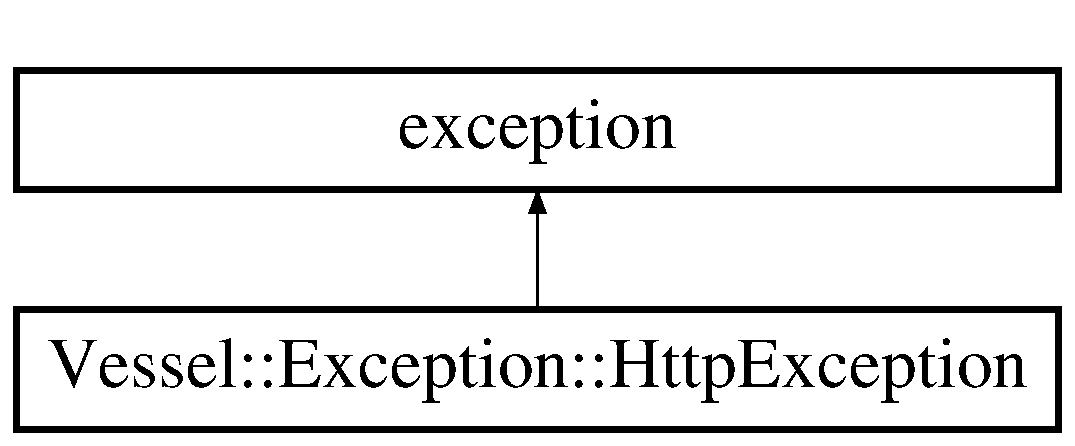
\includegraphics[height=2.000000cm]{class_vessel_1_1_exception_1_1_http_exception}
\end{center}
\end{figure}
\subsection*{Public Types}
\begin{DoxyCompactItemize}
\item 
\mbox{\Hypertarget{class_vessel_1_1_exception_1_1_http_exception_ae03e2b1c116d1758e87114e388ca22a7}\label{class_vessel_1_1_exception_1_1_http_exception_ae03e2b1c116d1758e87114e388ca22a7}} 
enum {\bfseries Error\+Code} \{ {\bfseries No\+Error} = 0, 
{\bfseries Invalid\+Url}, 
{\bfseries Connect\+Failed}, 
{\bfseries Handshake\+Failed}
 \}
\end{DoxyCompactItemize}
\subsection*{Public Member Functions}
\begin{DoxyCompactItemize}
\item 
\mbox{\Hypertarget{class_vessel_1_1_exception_1_1_http_exception_a909f1698f60eef57213bb1ec55086902}\label{class_vessel_1_1_exception_1_1_http_exception_a909f1698f60eef57213bb1ec55086902}} 
{\bfseries Http\+Exception} (Error\+Code e, const std\+::string \&msg)
\item 
\mbox{\Hypertarget{class_vessel_1_1_exception_1_1_http_exception_afbaa54b8a0ad67e2dd9dd0394f56a2df}\label{class_vessel_1_1_exception_1_1_http_exception_afbaa54b8a0ad67e2dd9dd0394f56a2df}} 
Error\+Code {\bfseries get\+\_\+code} ()
\item 
\mbox{\Hypertarget{class_vessel_1_1_exception_1_1_http_exception_ae3a5bb38fe59f763af267338804a0cef}\label{class_vessel_1_1_exception_1_1_http_exception_ae3a5bb38fe59f763af267338804a0cef}} 
virtual const char $\ast$ {\bfseries what} () const noexcept override
\end{DoxyCompactItemize}


The documentation for this class was generated from the following file\+:\begin{DoxyCompactItemize}
\item 
/home/kyle/cpp/bv-\/backup/include/vessel/network/http\+\_\+exception.\+hpp\end{DoxyCompactItemize}

\hypertarget{class_vessel_1_1_networking_1_1_http_request}{}\section{Vessel\+:\+:Networking\+:\+:Http\+Request Class Reference}
\label{class_vessel_1_1_networking_1_1_http_request}\index{Vessel\+::\+Networking\+::\+Http\+Request@{Vessel\+::\+Networking\+::\+Http\+Request}}
\subsection*{Public Member Functions}
\begin{DoxyCompactItemize}
\item 
\mbox{\Hypertarget{class_vessel_1_1_networking_1_1_http_request_a69e25a5c71c13bcf46cb042cbff8274b}\label{class_vessel_1_1_networking_1_1_http_request_a69e25a5c71c13bcf46cb042cbff8274b}} 
void {\bfseries set\+\_\+url} (const std\+::string \&str)
\item 
\mbox{\Hypertarget{class_vessel_1_1_networking_1_1_http_request_a01b5329f00d6270d98042cc5fd943c40}\label{class_vessel_1_1_networking_1_1_http_request_a01b5329f00d6270d98042cc5fd943c40}} 
void {\bfseries set\+\_\+method} (const std\+::string \&str)
\item 
\mbox{\Hypertarget{class_vessel_1_1_networking_1_1_http_request_a0edbd0445e9636e498a2a12807e6be18}\label{class_vessel_1_1_networking_1_1_http_request_a0edbd0445e9636e498a2a12807e6be18}} 
void {\bfseries add\+\_\+header} (const std\+::string \&str)
\item 
\mbox{\Hypertarget{class_vessel_1_1_networking_1_1_http_request_a4ef063a4e4d9d037f39194d502c491cd}\label{class_vessel_1_1_networking_1_1_http_request_a4ef063a4e4d9d037f39194d502c491cd}} 
void {\bfseries set\+\_\+content\+\_\+type} (const std\+::string \&str)
\item 
\mbox{\Hypertarget{class_vessel_1_1_networking_1_1_http_request_a6f2c55559d9bf22c18782a944210c63a}\label{class_vessel_1_1_networking_1_1_http_request_a6f2c55559d9bf22c18782a944210c63a}} 
void {\bfseries set\+\_\+body} (const std\+::string \&str)
\item 
\mbox{\Hypertarget{class_vessel_1_1_networking_1_1_http_request_a21e9d62ce0782cb8785a979b3bd04ae2}\label{class_vessel_1_1_networking_1_1_http_request_a21e9d62ce0782cb8785a979b3bd04ae2}} 
void {\bfseries set\+\_\+auth\+\_\+header} (const std\+::string \&str)
\item 
\mbox{\Hypertarget{class_vessel_1_1_networking_1_1_http_request_a6a84d3689dc11ac1b2f81ef64418452c}\label{class_vessel_1_1_networking_1_1_http_request_a6a84d3689dc11ac1b2f81ef64418452c}} 
void {\bfseries accept} (const std\+::string \&str)
\item 
\mbox{\Hypertarget{class_vessel_1_1_networking_1_1_http_request_aa50f669749dc7684b43fa80b03a4cea5}\label{class_vessel_1_1_networking_1_1_http_request_aa50f669749dc7684b43fa80b03a4cea5}} 
std\+::string {\bfseries get\+\_\+url} () const
\item 
\mbox{\Hypertarget{class_vessel_1_1_networking_1_1_http_request_ae87d59bf82a8dfb1d7fdbe5526933dbe}\label{class_vessel_1_1_networking_1_1_http_request_ae87d59bf82a8dfb1d7fdbe5526933dbe}} 
std\+::string {\bfseries get\+\_\+method} () const
\item 
\mbox{\Hypertarget{class_vessel_1_1_networking_1_1_http_request_a88b4b723f7a700b3a31239a2a5c1bf52}\label{class_vessel_1_1_networking_1_1_http_request_a88b4b723f7a700b3a31239a2a5c1bf52}} 
std\+::vector$<$ std\+::string $>$ {\bfseries get\+\_\+headers} () const
\item 
\mbox{\Hypertarget{class_vessel_1_1_networking_1_1_http_request_ace6fc0a7eed46ad501e9afdec4874cfc}\label{class_vessel_1_1_networking_1_1_http_request_ace6fc0a7eed46ad501e9afdec4874cfc}} 
std\+::string {\bfseries get\+\_\+content\+\_\+type} () const
\item 
\mbox{\Hypertarget{class_vessel_1_1_networking_1_1_http_request_a9d1a4115eb3eb1866bad739b0e9b0c3c}\label{class_vessel_1_1_networking_1_1_http_request_a9d1a4115eb3eb1866bad739b0e9b0c3c}} 
std\+::string {\bfseries get\+\_\+body} () const
\item 
\mbox{\Hypertarget{class_vessel_1_1_networking_1_1_http_request_af117db81f197b8cca5776e7c1c072aab}\label{class_vessel_1_1_networking_1_1_http_request_af117db81f197b8cca5776e7c1c072aab}} 
std\+::string {\bfseries get\+\_\+accept} () const
\item 
\mbox{\Hypertarget{class_vessel_1_1_networking_1_1_http_request_a81fa60d4bc862883aae195414880f9bd}\label{class_vessel_1_1_networking_1_1_http_request_a81fa60d4bc862883aae195414880f9bd}} 
std\+::string {\bfseries get\+\_\+auth} () const
\item 
\mbox{\Hypertarget{class_vessel_1_1_networking_1_1_http_request_ac1ce8c49c62282b69f9cb4180e3d2e50}\label{class_vessel_1_1_networking_1_1_http_request_ac1ce8c49c62282b69f9cb4180e3d2e50}} 
size\+\_\+t {\bfseries get\+\_\+body\+\_\+length} () const
\end{DoxyCompactItemize}


The documentation for this class was generated from the following file\+:\begin{DoxyCompactItemize}
\item 
/home/kyle/cpp/bv-\/backup/include/vessel/network/http\+\_\+request.\+hpp\end{DoxyCompactItemize}

\hypertarget{class_vessel_1_1_networking_1_1_http_request_stream}{}\section{Vessel\+:\+:Networking\+:\+:Http\+Request\+Stream Class Reference}
\label{class_vessel_1_1_networking_1_1_http_request_stream}\index{Vessel\+::\+Networking\+::\+Http\+Request\+Stream@{Vessel\+::\+Networking\+::\+Http\+Request\+Stream}}
\subsection*{Public Member Functions}
\begin{DoxyCompactItemize}
\item 
\mbox{\Hypertarget{class_vessel_1_1_networking_1_1_http_request_stream_a14a71737997cc7f73bbd3e33b43a659d}\label{class_vessel_1_1_networking_1_1_http_request_stream_a14a71737997cc7f73bbd3e33b43a659d}} 
{\bfseries Http\+Request\+Stream} (const std\+::string \&str)
\item 
\mbox{\Hypertarget{class_vessel_1_1_networking_1_1_http_request_stream_aaaf4033cf1223f0928706b8fbf00e85b}\label{class_vessel_1_1_networking_1_1_http_request_stream_aaaf4033cf1223f0928706b8fbf00e85b}} 
std\+::string {\bfseries str} () const
\item 
\mbox{\Hypertarget{class_vessel_1_1_networking_1_1_http_request_stream_af600015104b9426c5f2b276de0cc5ac9}\label{class_vessel_1_1_networking_1_1_http_request_stream_af600015104b9426c5f2b276de0cc5ac9}} 
std\+::string \& {\bfseries str} ()
\item 
\mbox{\Hypertarget{class_vessel_1_1_networking_1_1_http_request_stream_ac738ef27538c0f9e3b881cbf1f3edefc}\label{class_vessel_1_1_networking_1_1_http_request_stream_ac738ef27538c0f9e3b881cbf1f3edefc}} 
void {\bfseries append} (const std\+::string \&str)
\item 
\mbox{\Hypertarget{class_vessel_1_1_networking_1_1_http_request_stream_a01c538560d550ed4a2c7cd50e579b840}\label{class_vessel_1_1_networking_1_1_http_request_stream_a01c538560d550ed4a2c7cd50e579b840}} 
void {\bfseries append} (int num)
\end{DoxyCompactItemize}
\subsection*{Friends}
\begin{DoxyCompactItemize}
\item 
\mbox{\Hypertarget{class_vessel_1_1_networking_1_1_http_request_stream_a2d24d2c7425ac458c963bdc51059415c}\label{class_vessel_1_1_networking_1_1_http_request_stream_a2d24d2c7425ac458c963bdc51059415c}} 
\hyperlink{class_vessel_1_1_networking_1_1_http_request_stream}{Http\+Request\+Stream} \& {\bfseries operator$<$$<$} (\hyperlink{class_vessel_1_1_networking_1_1_http_request_stream}{Http\+Request\+Stream} \&rs, const std\+::string \&str)
\item 
\mbox{\Hypertarget{class_vessel_1_1_networking_1_1_http_request_stream_a7ff230dac2eb391d3a09f6338c5a7a73}\label{class_vessel_1_1_networking_1_1_http_request_stream_a7ff230dac2eb391d3a09f6338c5a7a73}} 
\hyperlink{class_vessel_1_1_networking_1_1_http_request_stream}{Http\+Request\+Stream} \& {\bfseries operator$<$$<$} (\hyperlink{class_vessel_1_1_networking_1_1_http_request_stream}{Http\+Request\+Stream} \&rs, int num)
\item 
\mbox{\Hypertarget{class_vessel_1_1_networking_1_1_http_request_stream_aafc07abcec7431466712ee2a45f95b70}\label{class_vessel_1_1_networking_1_1_http_request_stream_aafc07abcec7431466712ee2a45f95b70}} 
std\+::ostream \& {\bfseries operator$<$$<$} (std\+::ostream \&os, const std\+::string \&str)
\item 
\mbox{\Hypertarget{class_vessel_1_1_networking_1_1_http_request_stream_aa6b90dd91dd9c446c9238d631a3661a8}\label{class_vessel_1_1_networking_1_1_http_request_stream_aa6b90dd91dd9c446c9238d631a3661a8}} 
std\+::ostream \& {\bfseries operator$<$$<$} (std\+::ostream \&os, \hyperlink{class_vessel_1_1_networking_1_1_http_request_stream}{Http\+Request\+Stream} \&rs)
\item 
\mbox{\Hypertarget{class_vessel_1_1_networking_1_1_http_request_stream_af60ace94cdad2d7b5305db0fc6c92fd9}\label{class_vessel_1_1_networking_1_1_http_request_stream_af60ace94cdad2d7b5305db0fc6c92fd9}} 
std\+::istream \& {\bfseries operator$>$$>$} (std\+::istream \&is, std\+::string \&str)
\end{DoxyCompactItemize}


The documentation for this class was generated from the following file\+:\begin{DoxyCompactItemize}
\item 
/home/kyle/cpp/bv-\/backup/include/vessel/network/http\+\_\+stream.\+hpp\end{DoxyCompactItemize}

\hypertarget{class_vessel_1_1_database_1_1_local_database}{}\section{Vessel\+:\+:Database\+:\+:Local\+Database Class Reference}
\label{class_vessel_1_1_database_1_1_local_database}\index{Vessel\+::\+Database\+::\+Local\+Database@{Vessel\+::\+Database\+::\+Local\+Database}}
\subsection*{Public Member Functions}
\begin{DoxyCompactItemize}
\item 
\hyperlink{class_vessel_1_1_database_1_1_local_database_af2180ec115f920bb5cf9915da9873478}{Local\+Database} (\hyperlink{class_vessel_1_1_database_1_1_local_database}{Local\+Database} const \&)=delete
\item 
\mbox{\Hypertarget{class_vessel_1_1_database_1_1_local_database_a498009e5019d6412452f763ea06515c1}\label{class_vessel_1_1_database_1_1_local_database_a498009e5019d6412452f763ea06515c1}} 
void {\bfseries operator=} (\hyperlink{class_vessel_1_1_database_1_1_local_database}{Local\+Database} const \&)=delete
\item 
sqlite3 $\ast$ \hyperlink{class_vessel_1_1_database_1_1_local_database_a7df737694e981572b00a3a9b9d0a7eeb}{get\+\_\+handle} ()
\begin{DoxyCompactList}\small\item\em Returns a handle to the sqlite database. \end{DoxyCompactList}\item 
std\+::string \hyperlink{class_vessel_1_1_database_1_1_local_database_aaeca7268517cb884b7aa7ea4b7f3db04}{get\+\_\+setting\+\_\+str} (const std\+::string \&s)
\begin{DoxyCompactList}\small\item\em Returns string value of a setting from the Database. \end{DoxyCompactList}\item 
int \hyperlink{class_vessel_1_1_database_1_1_local_database_af37832c98d2e9eabe40b2a45f5035133}{get\+\_\+setting\+\_\+int} (const std\+::string \&s)
\begin{DoxyCompactList}\small\item\em Returns int value of a setting from the Database. \end{DoxyCompactList}\item 
{\footnotesize template$<$typename T $>$ }\\bool \hyperlink{class_vessel_1_1_database_1_1_local_database_a94da226c9c5561a4cb88290c6aa334a3}{update\+\_\+setting} (const std\+::string \&key, const T \&val)
\begin{DoxyCompactList}\small\item\em Updates a setting value in the database. \end{DoxyCompactList}\item 
\mbox{\Hypertarget{class_vessel_1_1_database_1_1_local_database_a6894636c19e4781f619b2f6a50ae7994}\label{class_vessel_1_1_database_1_1_local_database_a6894636c19e4781f619b2f6a50ae7994}} 
bool {\bfseries update\+\_\+ext\+\_\+count} (const std\+::string \&ext, int total)
\item 
std\+::string \hyperlink{class_vessel_1_1_database_1_1_local_database_a2604bed46b522977ba77140626282f3d}{get\+\_\+last\+\_\+err} ()
\begin{DoxyCompactList}\small\item\em Returns the last error from the database (if any) \end{DoxyCompactList}\item 
\mbox{\Hypertarget{class_vessel_1_1_database_1_1_local_database_ac8639c0eb1ed8757b080de38e0314222}\label{class_vessel_1_1_database_1_1_local_database_ac8639c0eb1ed8757b080de38e0314222}} 
void \hyperlink{class_vessel_1_1_database_1_1_local_database_ac8639c0eb1ed8757b080de38e0314222}{update\+\_\+global\+\_\+settings} ()
\begin{DoxyCompactList}\small\item\em Updates global environment settings. \end{DoxyCompactList}\item 
\mbox{\Hypertarget{class_vessel_1_1_database_1_1_local_database_ae43917bc8ebb0f0269da1ac68685a040}\label{class_vessel_1_1_database_1_1_local_database_ae43917bc8ebb0f0269da1ac68685a040}} 
void \hyperlink{class_vessel_1_1_database_1_1_local_database_ae43917bc8ebb0f0269da1ac68685a040}{update\+\_\+client\+\_\+settings} (const std\+::string \&s)
\begin{DoxyCompactList}\small\item\em Parses client settings J\+S\+ON from Vessel R\+E\+ST A\+PI and saves to database. \end{DoxyCompactList}\item 
\mbox{\Hypertarget{class_vessel_1_1_database_1_1_local_database_a4863f63ed1a6ad1dbbcce0208759a5d7}\label{class_vessel_1_1_database_1_1_local_database_a4863f63ed1a6ad1dbbcce0208759a5d7}} 
void \hyperlink{class_vessel_1_1_database_1_1_local_database_a4863f63ed1a6ad1dbbcce0208759a5d7}{clean} ()
\begin{DoxyCompactList}\small\item\em Scans the directory and file table for non-\/existent files/directories and removes them from the database. \end{DoxyCompactList}\item 
\mbox{\Hypertarget{class_vessel_1_1_database_1_1_local_database_a1a5348e3de490bb8b1fb7c923dc5d9de}\label{class_vessel_1_1_database_1_1_local_database_a1a5348e3de490bb8b1fb7c923dc5d9de}} 
void \hyperlink{class_vessel_1_1_database_1_1_local_database_a1a5348e3de490bb8b1fb7c923dc5d9de}{start\+\_\+transaction} ()
\begin{DoxyCompactList}\small\item\em Starts a database transaction. \end{DoxyCompactList}\item 
\mbox{\Hypertarget{class_vessel_1_1_database_1_1_local_database_aae0ba68d8107d44d7fdc1137675ff0c6}\label{class_vessel_1_1_database_1_1_local_database_aae0ba68d8107d44d7fdc1137675ff0c6}} 
void \hyperlink{class_vessel_1_1_database_1_1_local_database_aae0ba68d8107d44d7fdc1137675ff0c6}{end\+\_\+transaction} ()
\begin{DoxyCompactList}\small\item\em Ends a database transaction. \end{DoxyCompactList}\item 
void \hyperlink{class_vessel_1_1_database_1_1_local_database_ab6315c29e00efda7ac808f68a054f0ea}{purge\+\_\+file} (unsigned char $\ast$file\+\_\+id)
\begin{DoxyCompactList}\small\item\em Removes a file from the database. \end{DoxyCompactList}\item 
void \hyperlink{class_vessel_1_1_database_1_1_local_database_a328b2ea5ed242bacc70ea6bf248bf44d}{purge\+\_\+upload} (unsigned int upload\+\_\+id)
\begin{DoxyCompactList}\small\item\em Removes an upload from the database. \end{DoxyCompactList}\item 
std\+::map$<$ std\+::string, int $>$ \hyperlink{class_vessel_1_1_database_1_1_local_database_ab55e12266822635ba8d4e74b9ca17a7d}{get\+\_\+stats} ()
\end{DoxyCompactItemize}
\subsection*{Static Public Member Functions}
\begin{DoxyCompactItemize}
\item 
static \hyperlink{class_vessel_1_1_database_1_1_local_database}{Local\+Database} \& \hyperlink{class_vessel_1_1_database_1_1_local_database_ad5d9f9dda2ad243ca640f7cf07de34d7}{get\+\_\+database} ()
\begin{DoxyCompactList}\small\item\em Static singleton factory constructor which returns an instance to \hyperlink{class_vessel_1_1_database_1_1_local_database}{Local\+Database}. \end{DoxyCompactList}\item 
static std\+::string \hyperlink{class_vessel_1_1_database_1_1_local_database_a1561145d386751e09b23b80a723735c4}{get\+\_\+sqlite\+\_\+str} (const void $\ast$data)
\begin{DoxyCompactList}\small\item\em Wrapper for sqlite3\+\_\+column\+\_\+text which prevents a segfault if N\+U\+LL is returned from the database. \end{DoxyCompactList}\item 
static std\+::shared\+\_\+ptr$<$ unsigned char $>$ \hyperlink{class_vessel_1_1_database_1_1_local_database_a2fabf54b26f3d3b0b29b1a682f8ed718}{get\+\_\+binary\+\_\+id} (unsigned char $\ast$id)
\begin{DoxyCompactList}\small\item\em Makes a copy of a binary id and returns a shared\+\_\+ptr of the copy. \end{DoxyCompactList}\end{DoxyCompactItemize}


\subsection{Constructor \& Destructor Documentation}
\mbox{\Hypertarget{class_vessel_1_1_database_1_1_local_database_af2180ec115f920bb5cf9915da9873478}\label{class_vessel_1_1_database_1_1_local_database_af2180ec115f920bb5cf9915da9873478}} 
\index{Vessel\+::\+Database\+::\+Local\+Database@{Vessel\+::\+Database\+::\+Local\+Database}!Local\+Database@{Local\+Database}}
\index{Local\+Database@{Local\+Database}!Vessel\+::\+Database\+::\+Local\+Database@{Vessel\+::\+Database\+::\+Local\+Database}}
\subsubsection{\texorpdfstring{Local\+Database()}{LocalDatabase()}}
{\footnotesize\ttfamily Vessel\+::\+Database\+::\+Local\+Database\+::\+Local\+Database (\begin{DoxyParamCaption}\item[{\hyperlink{class_vessel_1_1_database_1_1_local_database}{Local\+Database} const \&}]{ }\end{DoxyParamCaption})\hspace{0.3cm}{\ttfamily [delete]}}

No Assignment or Copies allowed 

\subsection{Member Function Documentation}
\mbox{\Hypertarget{class_vessel_1_1_database_1_1_local_database_a2fabf54b26f3d3b0b29b1a682f8ed718}\label{class_vessel_1_1_database_1_1_local_database_a2fabf54b26f3d3b0b29b1a682f8ed718}} 
\index{Vessel\+::\+Database\+::\+Local\+Database@{Vessel\+::\+Database\+::\+Local\+Database}!get\+\_\+binary\+\_\+id@{get\+\_\+binary\+\_\+id}}
\index{get\+\_\+binary\+\_\+id@{get\+\_\+binary\+\_\+id}!Vessel\+::\+Database\+::\+Local\+Database@{Vessel\+::\+Database\+::\+Local\+Database}}
\subsubsection{\texorpdfstring{get\+\_\+binary\+\_\+id()}{get\_binary\_id()}}
{\footnotesize\ttfamily static std\+::shared\+\_\+ptr$<$ unsigned char $>$ Vessel\+::\+Database\+::\+Local\+Database\+::get\+\_\+binary\+\_\+id (\begin{DoxyParamCaption}\item[{unsigned char $\ast$}]{id }\end{DoxyParamCaption})\hspace{0.3cm}{\ttfamily [static]}}



Makes a copy of a binary id and returns a shared\+\_\+ptr of the copy. 


\begin{DoxyParams}{Parameters}
{\em id} & Some binary/raw id \\
\hline
\end{DoxyParams}
\mbox{\Hypertarget{class_vessel_1_1_database_1_1_local_database_ad5d9f9dda2ad243ca640f7cf07de34d7}\label{class_vessel_1_1_database_1_1_local_database_ad5d9f9dda2ad243ca640f7cf07de34d7}} 
\index{Vessel\+::\+Database\+::\+Local\+Database@{Vessel\+::\+Database\+::\+Local\+Database}!get\+\_\+database@{get\+\_\+database}}
\index{get\+\_\+database@{get\+\_\+database}!Vessel\+::\+Database\+::\+Local\+Database@{Vessel\+::\+Database\+::\+Local\+Database}}
\subsubsection{\texorpdfstring{get\+\_\+database()}{get\_database()}}
{\footnotesize\ttfamily static \hyperlink{class_vessel_1_1_database_1_1_local_database}{Local\+Database} \& Vessel\+::\+Database\+::\+Local\+Database\+::get\+\_\+database (\begin{DoxyParamCaption}{ }\end{DoxyParamCaption})\hspace{0.3cm}{\ttfamily [inline]}, {\ttfamily [static]}}



Static singleton factory constructor which returns an instance to \hyperlink{class_vessel_1_1_database_1_1_local_database}{Local\+Database}. 

\begin{DoxyReturn}{Returns}
Singleton instance to \hyperlink{class_vessel_1_1_database_1_1_local_database}{Local\+Database} 
\end{DoxyReturn}
\mbox{\Hypertarget{class_vessel_1_1_database_1_1_local_database_a7df737694e981572b00a3a9b9d0a7eeb}\label{class_vessel_1_1_database_1_1_local_database_a7df737694e981572b00a3a9b9d0a7eeb}} 
\index{Vessel\+::\+Database\+::\+Local\+Database@{Vessel\+::\+Database\+::\+Local\+Database}!get\+\_\+handle@{get\+\_\+handle}}
\index{get\+\_\+handle@{get\+\_\+handle}!Vessel\+::\+Database\+::\+Local\+Database@{Vessel\+::\+Database\+::\+Local\+Database}}
\subsubsection{\texorpdfstring{get\+\_\+handle()}{get\_handle()}}
{\footnotesize\ttfamily sqlite3 $\ast$ Vessel\+::\+Database\+::\+Local\+Database\+::get\+\_\+handle (\begin{DoxyParamCaption}{ }\end{DoxyParamCaption})}



Returns a handle to the sqlite database. 

\begin{DoxyReturn}{Returns}
Returns a handle to the sqlite database 
\end{DoxyReturn}
\mbox{\Hypertarget{class_vessel_1_1_database_1_1_local_database_a2604bed46b522977ba77140626282f3d}\label{class_vessel_1_1_database_1_1_local_database_a2604bed46b522977ba77140626282f3d}} 
\index{Vessel\+::\+Database\+::\+Local\+Database@{Vessel\+::\+Database\+::\+Local\+Database}!get\+\_\+last\+\_\+err@{get\+\_\+last\+\_\+err}}
\index{get\+\_\+last\+\_\+err@{get\+\_\+last\+\_\+err}!Vessel\+::\+Database\+::\+Local\+Database@{Vessel\+::\+Database\+::\+Local\+Database}}
\subsubsection{\texorpdfstring{get\+\_\+last\+\_\+err()}{get\_last\_err()}}
{\footnotesize\ttfamily std\+::string Vessel\+::\+Database\+::\+Local\+Database\+::get\+\_\+last\+\_\+err (\begin{DoxyParamCaption}{ }\end{DoxyParamCaption})}



Returns the last error from the database (if any) 

\begin{DoxyReturn}{Returns}
Returns the last error from the database (if any) 
\end{DoxyReturn}
\mbox{\Hypertarget{class_vessel_1_1_database_1_1_local_database_af37832c98d2e9eabe40b2a45f5035133}\label{class_vessel_1_1_database_1_1_local_database_af37832c98d2e9eabe40b2a45f5035133}} 
\index{Vessel\+::\+Database\+::\+Local\+Database@{Vessel\+::\+Database\+::\+Local\+Database}!get\+\_\+setting\+\_\+int@{get\+\_\+setting\+\_\+int}}
\index{get\+\_\+setting\+\_\+int@{get\+\_\+setting\+\_\+int}!Vessel\+::\+Database\+::\+Local\+Database@{Vessel\+::\+Database\+::\+Local\+Database}}
\subsubsection{\texorpdfstring{get\+\_\+setting\+\_\+int()}{get\_setting\_int()}}
{\footnotesize\ttfamily int Vessel\+::\+Database\+::\+Local\+Database\+::get\+\_\+setting\+\_\+int (\begin{DoxyParamCaption}\item[{const std\+::string \&}]{s }\end{DoxyParamCaption})}



Returns int value of a setting from the Database. 


\begin{DoxyParams}{Parameters}
{\em s} & Name of the setting to retrieve \\
\hline
\end{DoxyParams}
\begin{DoxyReturn}{Returns}
Returns int value of a setting from the Database 
\end{DoxyReturn}
\mbox{\Hypertarget{class_vessel_1_1_database_1_1_local_database_aaeca7268517cb884b7aa7ea4b7f3db04}\label{class_vessel_1_1_database_1_1_local_database_aaeca7268517cb884b7aa7ea4b7f3db04}} 
\index{Vessel\+::\+Database\+::\+Local\+Database@{Vessel\+::\+Database\+::\+Local\+Database}!get\+\_\+setting\+\_\+str@{get\+\_\+setting\+\_\+str}}
\index{get\+\_\+setting\+\_\+str@{get\+\_\+setting\+\_\+str}!Vessel\+::\+Database\+::\+Local\+Database@{Vessel\+::\+Database\+::\+Local\+Database}}
\subsubsection{\texorpdfstring{get\+\_\+setting\+\_\+str()}{get\_setting\_str()}}
{\footnotesize\ttfamily std\+::string Vessel\+::\+Database\+::\+Local\+Database\+::get\+\_\+setting\+\_\+str (\begin{DoxyParamCaption}\item[{const std\+::string \&}]{s }\end{DoxyParamCaption})}



Returns string value of a setting from the Database. 


\begin{DoxyParams}{Parameters}
{\em s} & Name of the setting to retrieve \\
\hline
\end{DoxyParams}
\begin{DoxyReturn}{Returns}
Returns string value of a setting from the Database 
\end{DoxyReturn}
\mbox{\Hypertarget{class_vessel_1_1_database_1_1_local_database_a1561145d386751e09b23b80a723735c4}\label{class_vessel_1_1_database_1_1_local_database_a1561145d386751e09b23b80a723735c4}} 
\index{Vessel\+::\+Database\+::\+Local\+Database@{Vessel\+::\+Database\+::\+Local\+Database}!get\+\_\+sqlite\+\_\+str@{get\+\_\+sqlite\+\_\+str}}
\index{get\+\_\+sqlite\+\_\+str@{get\+\_\+sqlite\+\_\+str}!Vessel\+::\+Database\+::\+Local\+Database@{Vessel\+::\+Database\+::\+Local\+Database}}
\subsubsection{\texorpdfstring{get\+\_\+sqlite\+\_\+str()}{get\_sqlite\_str()}}
{\footnotesize\ttfamily static std\+::string Vessel\+::\+Database\+::\+Local\+Database\+::get\+\_\+sqlite\+\_\+str (\begin{DoxyParamCaption}\item[{const void $\ast$}]{data }\end{DoxyParamCaption})\hspace{0.3cm}{\ttfamily [static]}}



Wrapper for sqlite3\+\_\+column\+\_\+text which prevents a segfault if N\+U\+LL is returned from the database. 

\begin{DoxyReturn}{Returns}
Returns the string value from the database, or empty string if N\+U\+LL 
\end{DoxyReturn}
\mbox{\Hypertarget{class_vessel_1_1_database_1_1_local_database_ab55e12266822635ba8d4e74b9ca17a7d}\label{class_vessel_1_1_database_1_1_local_database_ab55e12266822635ba8d4e74b9ca17a7d}} 
\index{Vessel\+::\+Database\+::\+Local\+Database@{Vessel\+::\+Database\+::\+Local\+Database}!get\+\_\+stats@{get\+\_\+stats}}
\index{get\+\_\+stats@{get\+\_\+stats}!Vessel\+::\+Database\+::\+Local\+Database@{Vessel\+::\+Database\+::\+Local\+Database}}
\subsubsection{\texorpdfstring{get\+\_\+stats()}{get\_stats()}}
{\footnotesize\ttfamily std\+::map$<$ std\+::string, int $>$ Vessel\+::\+Database\+::\+Local\+Database\+::get\+\_\+stats (\begin{DoxyParamCaption}{ }\end{DoxyParamCaption})}

\begin{DoxyReturn}{Returns}
Returns a vector of stat key/value pairs 
\end{DoxyReturn}
\mbox{\Hypertarget{class_vessel_1_1_database_1_1_local_database_ab6315c29e00efda7ac808f68a054f0ea}\label{class_vessel_1_1_database_1_1_local_database_ab6315c29e00efda7ac808f68a054f0ea}} 
\index{Vessel\+::\+Database\+::\+Local\+Database@{Vessel\+::\+Database\+::\+Local\+Database}!purge\+\_\+file@{purge\+\_\+file}}
\index{purge\+\_\+file@{purge\+\_\+file}!Vessel\+::\+Database\+::\+Local\+Database@{Vessel\+::\+Database\+::\+Local\+Database}}
\subsubsection{\texorpdfstring{purge\+\_\+file()}{purge\_file()}}
{\footnotesize\ttfamily void Vessel\+::\+Database\+::\+Local\+Database\+::purge\+\_\+file (\begin{DoxyParamCaption}\item[{unsigned char $\ast$}]{file\+\_\+id }\end{DoxyParamCaption})}



Removes a file from the database. 


\begin{DoxyParams}{Parameters}
{\em file\+\_\+id} & Binary File ID \\
\hline
\end{DoxyParams}
\mbox{\Hypertarget{class_vessel_1_1_database_1_1_local_database_a328b2ea5ed242bacc70ea6bf248bf44d}\label{class_vessel_1_1_database_1_1_local_database_a328b2ea5ed242bacc70ea6bf248bf44d}} 
\index{Vessel\+::\+Database\+::\+Local\+Database@{Vessel\+::\+Database\+::\+Local\+Database}!purge\+\_\+upload@{purge\+\_\+upload}}
\index{purge\+\_\+upload@{purge\+\_\+upload}!Vessel\+::\+Database\+::\+Local\+Database@{Vessel\+::\+Database\+::\+Local\+Database}}
\subsubsection{\texorpdfstring{purge\+\_\+upload()}{purge\_upload()}}
{\footnotesize\ttfamily void Vessel\+::\+Database\+::\+Local\+Database\+::purge\+\_\+upload (\begin{DoxyParamCaption}\item[{unsigned int}]{upload\+\_\+id }\end{DoxyParamCaption})}



Removes an upload from the database. 


\begin{DoxyParams}{Parameters}
{\em upload\+\_\+id} & Database Upload Id \\
\hline
\end{DoxyParams}
\mbox{\Hypertarget{class_vessel_1_1_database_1_1_local_database_a94da226c9c5561a4cb88290c6aa334a3}\label{class_vessel_1_1_database_1_1_local_database_a94da226c9c5561a4cb88290c6aa334a3}} 
\index{Vessel\+::\+Database\+::\+Local\+Database@{Vessel\+::\+Database\+::\+Local\+Database}!update\+\_\+setting@{update\+\_\+setting}}
\index{update\+\_\+setting@{update\+\_\+setting}!Vessel\+::\+Database\+::\+Local\+Database@{Vessel\+::\+Database\+::\+Local\+Database}}
\subsubsection{\texorpdfstring{update\+\_\+setting()}{update\_setting()}}
{\footnotesize\ttfamily template$<$typename T $>$ \\
bool Vessel\+::\+Database\+::\+Local\+Database\+::update\+\_\+setting (\begin{DoxyParamCaption}\item[{const std\+::string \&}]{key,  }\item[{const T \&}]{val }\end{DoxyParamCaption})}



Updates a setting value in the database. 


\begin{DoxyParams}{Parameters}
{\em key} & Name of the setting to update \\
\hline
{\em val} & New value of the setting \\
\hline
\end{DoxyParams}
\begin{DoxyReturn}{Returns}
Returns true if updated successfully 
\end{DoxyReturn}


The documentation for this class was generated from the following file\+:\begin{DoxyCompactItemize}
\item 
/home/kyle/cpp/bv-\/backup/include/vessel/database/local\+\_\+db.\+hpp\end{DoxyCompactItemize}

\hypertarget{class_vessel_1_1_logging_1_1_log}{}\section{Vessel\+:\+:Logging\+:\+:Log Class Reference}
\label{class_vessel_1_1_logging_1_1_log}\index{Vessel\+::\+Logging\+::\+Log@{Vessel\+::\+Logging\+::\+Log}}
\subsection*{Public Member Functions}
\begin{DoxyCompactItemize}
\item 
\mbox{\Hypertarget{class_vessel_1_1_logging_1_1_log_a1efbbd38289c6c5408c763496328cc83}\label{class_vessel_1_1_logging_1_1_log_a1efbbd38289c6c5408c763496328cc83}} 
{\bfseries Log} (\hyperlink{class_vessel_1_1_logging_1_1_log}{Log} const \&)=delete
\item 
\mbox{\Hypertarget{class_vessel_1_1_logging_1_1_log_a13b25b6f58b6d14e3eb2925f2eaafd26}\label{class_vessel_1_1_logging_1_1_log_a13b25b6f58b6d14e3eb2925f2eaafd26}} 
void {\bfseries operator=} (\hyperlink{class_vessel_1_1_logging_1_1_log}{Log} const \&)=delete
\item 
\mbox{\Hypertarget{class_vessel_1_1_logging_1_1_log_a836168fc70cf2f6901b42375644eb357}\label{class_vessel_1_1_logging_1_1_log_a836168fc70cf2f6901b42375644eb357}} 
void {\bfseries add\+\_\+message} (const std\+::string \&msg, const std\+::string \&type)
\item 
\mbox{\Hypertarget{class_vessel_1_1_logging_1_1_log_a835a3c775891e4b37a3363b9dc656bdf}\label{class_vessel_1_1_logging_1_1_log_a835a3c775891e4b37a3363b9dc656bdf}} 
void {\bfseries add\+\_\+error} (const std\+::string \&msg, const std\+::string \&type)
\item 
\mbox{\Hypertarget{class_vessel_1_1_logging_1_1_log_a7fb574e36c7728c8e8e18d7926509ea8}\label{class_vessel_1_1_logging_1_1_log_a7fb574e36c7728c8e8e18d7926509ea8}} 
void {\bfseries add\+\_\+http\+\_\+message} (const std\+::string \&request, const std\+::string \&response, int status)
\item 
\mbox{\Hypertarget{class_vessel_1_1_logging_1_1_log_a4ab1d8a2eee54eabb36e4e11b66d2ef0}\label{class_vessel_1_1_logging_1_1_log_a4ab1d8a2eee54eabb36e4e11b66d2ef0}} 
void {\bfseries add\+\_\+sql\+\_\+message} (const std\+::string \&msg, const std\+::string \&type, bool is\+\_\+error=false)
\item 
\mbox{\Hypertarget{class_vessel_1_1_logging_1_1_log_a85b0112150cb93282451f88602060ecb}\label{class_vessel_1_1_logging_1_1_log_a85b0112150cb93282451f88602060ecb}} 
void {\bfseries set\+\_\+level} (unsigned int level)
\item 
\mbox{\Hypertarget{class_vessel_1_1_logging_1_1_log_a405aea446f8a5e435f2ad42937b5b692}\label{class_vessel_1_1_logging_1_1_log_a405aea446f8a5e435f2ad42937b5b692}} 
void {\bfseries add\+\_\+exception} (const std\+::exception \&ex)
\item 
\mbox{\Hypertarget{class_vessel_1_1_logging_1_1_log_a07f5bdf65c8486bbc0435ec2aea89268}\label{class_vessel_1_1_logging_1_1_log_a07f5bdf65c8486bbc0435ec2aea89268}} 
void {\bfseries set\+\_\+file\+\_\+logging} (bool flag)
\item 
\mbox{\Hypertarget{class_vessel_1_1_logging_1_1_log_abe368762856fa1a3d35d42d2fdf58127}\label{class_vessel_1_1_logging_1_1_log_abe368762856fa1a3d35d42d2fdf58127}} 
void {\bfseries set\+\_\+sql\+\_\+logging} (bool flag)
\item 
\mbox{\Hypertarget{class_vessel_1_1_logging_1_1_log_a7b042407715512a34df83180594f28d0}\label{class_vessel_1_1_logging_1_1_log_a7b042407715512a34df83180594f28d0}} 
void {\bfseries set\+\_\+filename} (const std\+::string \&filename)
\end{DoxyCompactItemize}
\subsection*{Static Public Member Functions}
\begin{DoxyCompactItemize}
\item 
\mbox{\Hypertarget{class_vessel_1_1_logging_1_1_log_a58190201c41f0a3bb4ce7a5058abf949}\label{class_vessel_1_1_logging_1_1_log_a58190201c41f0a3bb4ce7a5058abf949}} 
static \hyperlink{class_vessel_1_1_logging_1_1_log}{Log} \& {\bfseries get\+\_\+log} ()
\end{DoxyCompactItemize}


The documentation for this class was generated from the following file\+:\begin{DoxyCompactItemize}
\item 
/home/kyle/cpp/bv-\/backup/include/vessel/log/log.\+hpp\end{DoxyCompactItemize}

\hypertarget{class_vessel_1_1_queue_manager}{}\section{Vessel\+:\+:Queue\+Manager Class Reference}
\label{class_vessel_1_1_queue_manager}\index{Vessel\+::\+Queue\+Manager@{Vessel\+::\+Queue\+Manager}}
\subsection*{Public Member Functions}
\begin{DoxyCompactItemize}
\item 
\mbox{\Hypertarget{class_vessel_1_1_queue_manager_af1a072eaf9108bea0266a08b042ab252}\label{class_vessel_1_1_queue_manager_af1a072eaf9108bea0266a08b042ab252}} 
\hyperlink{class_vessel_1_1_file_1_1_backup_file}{Backup\+File} {\bfseries get\+\_\+next\+\_\+file} ()
\item 
\mbox{\Hypertarget{class_vessel_1_1_queue_manager_a8a6de1b9b302492c4338972bd3317d85}\label{class_vessel_1_1_queue_manager_a8a6de1b9b302492c4338972bd3317d85}} 
\hyperlink{class_vessel_1_1_file_1_1_file_upload}{File\+Upload} {\bfseries get\+\_\+next\+\_\+upload} ()
\item 
\mbox{\Hypertarget{class_vessel_1_1_queue_manager_a4f3542c47ab942e96c0ef98c5fb211a0}\label{class_vessel_1_1_queue_manager_a4f3542c47ab942e96c0ef98c5fb211a0}} 
int {\bfseries get\+\_\+total\+\_\+pending} ()
\item 
\mbox{\Hypertarget{class_vessel_1_1_queue_manager_a1e531c84c86275602b9408a0b3610a5a}\label{class_vessel_1_1_queue_manager_a1e531c84c86275602b9408a0b3610a5a}} 
void {\bfseries rebuild\+\_\+queue} ()
\item 
\mbox{\Hypertarget{class_vessel_1_1_queue_manager_a3dfc89163a5c341b97e5ee5e5f31521a}\label{class_vessel_1_1_queue_manager_a3dfc89163a5c341b97e5ee5e5f31521a}} 
void {\bfseries pop\+\_\+file} (std\+::shared\+\_\+ptr$<$ unsigned char $>$ file\+\_\+id)
\end{DoxyCompactItemize}
\subsection*{Protected Member Functions}
\begin{DoxyCompactItemize}
\item 
\mbox{\Hypertarget{class_vessel_1_1_queue_manager_a47b7e3dd74d0580204fd8ee37e099f99}\label{class_vessel_1_1_queue_manager_a47b7e3dd74d0580204fd8ee37e099f99}} 
void {\bfseries clear\+\_\+queue} ()
\end{DoxyCompactItemize}


The documentation for this class was generated from the following file\+:\begin{DoxyCompactItemize}
\item 
/home/kyle/cpp/bv-\/backup/include/vessel/vessel/queue\+\_\+manager.\+hpp\end{DoxyCompactItemize}

\hypertarget{class_vessel_1_1_stat_manager}{}\section{Vessel\+:\+:Stat\+Manager Class Reference}
\label{class_vessel_1_1_stat_manager}\index{Vessel\+::\+Stat\+Manager@{Vessel\+::\+Stat\+Manager}}
\subsection*{Public Member Functions}
\begin{DoxyCompactItemize}
\item 
\mbox{\Hypertarget{class_vessel_1_1_stat_manager_a262852c31380b031464e78f7b3f5d6b3}\label{class_vessel_1_1_stat_manager_a262852c31380b031464e78f7b3f5d6b3}} 
void {\bfseries build\+\_\+stats} ()
\item 
\mbox{\Hypertarget{class_vessel_1_1_stat_manager_abc19fb509e44ee43998cfc44820595ce}\label{class_vessel_1_1_stat_manager_abc19fb509e44ee43998cfc44820595ce}} 
int {\bfseries get\+\_\+stat} (const std\+::string \&name)
\item 
\mbox{\Hypertarget{class_vessel_1_1_stat_manager_a9ba260d63f5323fda8a6bdc2ae2c2644}\label{class_vessel_1_1_stat_manager_a9ba260d63f5323fda8a6bdc2ae2c2644}} 
void {\bfseries update\+\_\+stat} (const std\+::string \&name, int value)
\end{DoxyCompactItemize}


The documentation for this class was generated from the following file\+:\begin{DoxyCompactItemize}
\item 
/home/kyle/cpp/bv-\/backup/include/vessel/vessel/stat\+\_\+manager.\+hpp\end{DoxyCompactItemize}

\hypertarget{struct_vessel_1_1_types_1_1_storage_provider}{}\section{Vessel\+:\+:Types\+:\+:Storage\+Provider Struct Reference}
\label{struct_vessel_1_1_types_1_1_storage_provider}\index{Vessel\+::\+Types\+::\+Storage\+Provider@{Vessel\+::\+Types\+::\+Storage\+Provider}}
\subsection*{Public Attributes}
\begin{DoxyCompactItemize}
\item 
\mbox{\Hypertarget{struct_vessel_1_1_types_1_1_storage_provider_a962cfc115daa3f6e963fb7e72b55c454}\label{struct_vessel_1_1_types_1_1_storage_provider_a962cfc115daa3f6e963fb7e72b55c454}} 
std\+::string {\bfseries provider\+\_\+id}
\item 
\mbox{\Hypertarget{struct_vessel_1_1_types_1_1_storage_provider_a065fa63ae96ee48405e8b74684578b64}\label{struct_vessel_1_1_types_1_1_storage_provider_a065fa63ae96ee48405e8b74684578b64}} 
std\+::string {\bfseries provider\+\_\+name}
\item 
\mbox{\Hypertarget{struct_vessel_1_1_types_1_1_storage_provider_ab8e1ef210e27d2667d0454a6b4e7127e}\label{struct_vessel_1_1_types_1_1_storage_provider_ab8e1ef210e27d2667d0454a6b4e7127e}} 
std\+::string {\bfseries description}
\item 
\mbox{\Hypertarget{struct_vessel_1_1_types_1_1_storage_provider_a6357453e0f626759a9230c800ddec3e4}\label{struct_vessel_1_1_types_1_1_storage_provider_a6357453e0f626759a9230c800ddec3e4}} 
std\+::string {\bfseries server}
\item 
\mbox{\Hypertarget{struct_vessel_1_1_types_1_1_storage_provider_ad30e41a94fbac78cc1fdfd9c46ca7fcc}\label{struct_vessel_1_1_types_1_1_storage_provider_ad30e41a94fbac78cc1fdfd9c46ca7fcc}} 
std\+::string {\bfseries access\+\_\+id}
\item 
\mbox{\Hypertarget{struct_vessel_1_1_types_1_1_storage_provider_a3363c79613348bf1a6c2bd562c476181}\label{struct_vessel_1_1_types_1_1_storage_provider_a3363c79613348bf1a6c2bd562c476181}} 
std\+::string {\bfseries access\+\_\+key}
\item 
\mbox{\Hypertarget{struct_vessel_1_1_types_1_1_storage_provider_af482e204357e832d7a3c4959543fcef7}\label{struct_vessel_1_1_types_1_1_storage_provider_af482e204357e832d7a3c4959543fcef7}} 
std\+::string {\bfseries region}
\item 
\mbox{\Hypertarget{struct_vessel_1_1_types_1_1_storage_provider_acf67fc655f9485b6f0487829688e5167}\label{struct_vessel_1_1_types_1_1_storage_provider_acf67fc655f9485b6f0487829688e5167}} 
std\+::string {\bfseries bucket\+\_\+name}
\item 
\mbox{\Hypertarget{struct_vessel_1_1_types_1_1_storage_provider_a50be99e6a3632625c7dc4cc0d82e52ca}\label{struct_vessel_1_1_types_1_1_storage_provider_a50be99e6a3632625c7dc4cc0d82e52ca}} 
std\+::string {\bfseries storage\+\_\+path}
\item 
\mbox{\Hypertarget{struct_vessel_1_1_types_1_1_storage_provider_a5f78989282a78c14ebc8ebe2797725fd}\label{struct_vessel_1_1_types_1_1_storage_provider_a5f78989282a78c14ebc8ebe2797725fd}} 
std\+::string {\bfseries provider\+\_\+type}
\item 
\mbox{\Hypertarget{struct_vessel_1_1_types_1_1_storage_provider_ac608757c8fa426fb6b4513b020d56fe9}\label{struct_vessel_1_1_types_1_1_storage_provider_ac608757c8fa426fb6b4513b020d56fe9}} 
std\+::string {\bfseries endpoint}
\item 
\mbox{\Hypertarget{struct_vessel_1_1_types_1_1_storage_provider_a7e2918a97a10cf38f09126a7f70598e9}\label{struct_vessel_1_1_types_1_1_storage_provider_a7e2918a97a10cf38f09126a7f70598e9}} 
int {\bfseries priority}
\end{DoxyCompactItemize}


The documentation for this struct was generated from the following file\+:\begin{DoxyCompactItemize}
\item 
/home/kyle/cpp/bv-\/backup/include/vessel/types.\+hpp\end{DoxyCompactItemize}

\hypertarget{class_vessel_1_1_compression_1_1_tarball}{}\section{Vessel\+:\+:Compression\+:\+:Tarball Class Reference}
\label{class_vessel_1_1_compression_1_1_tarball}\index{Vessel\+::\+Compression\+::\+Tarball@{Vessel\+::\+Compression\+::\+Tarball}}
\subsection*{Public Member Functions}
\begin{DoxyCompactItemize}
\item 
\mbox{\Hypertarget{class_vessel_1_1_compression_1_1_tarball_a81c6c75d0b9ff0670e4c6793818d16d4}\label{class_vessel_1_1_compression_1_1_tarball_a81c6c75d0b9ff0670e4c6793818d16d4}} 
{\bfseries Tarball} (const std\+::string \&filename)
\item 
\mbox{\Hypertarget{class_vessel_1_1_compression_1_1_tarball_a15bb8690a84b83808ed9894258cfa1ee}\label{class_vessel_1_1_compression_1_1_tarball_a15bb8690a84b83808ed9894258cfa1ee}} 
void {\bfseries add\+\_\+file} (const std\+::string \&filename)
\item 
\mbox{\Hypertarget{class_vessel_1_1_compression_1_1_tarball_a2655faae4e6c34d8e610561e9ea0651d}\label{class_vessel_1_1_compression_1_1_tarball_a2655faae4e6c34d8e610561e9ea0651d}} 
void {\bfseries save\+\_\+tar} ()
\end{DoxyCompactItemize}


The documentation for this class was generated from the following file\+:\begin{DoxyCompactItemize}
\item 
/home/kyle/cpp/bv-\/backup/include/vessel/compression/tarball.\+hpp\end{DoxyCompactItemize}

\hypertarget{class_vessel_1_1_networking_1_1_token_bucket}{}\section{Vessel\+:\+:Networking\+:\+:Token\+Bucket Class Reference}
\label{class_vessel_1_1_networking_1_1_token_bucket}\index{Vessel\+::\+Networking\+::\+Token\+Bucket@{Vessel\+::\+Networking\+::\+Token\+Bucket}}
\subsection*{Public Member Functions}
\begin{DoxyCompactItemize}
\item 
\mbox{\Hypertarget{class_vessel_1_1_networking_1_1_token_bucket_a7145d9092752774e66941c2e835b4c31}\label{class_vessel_1_1_networking_1_1_token_bucket_a7145d9092752774e66941c2e835b4c31}} 
{\bfseries Token\+Bucket} (size\+\_\+t bytes\+\_\+per\+\_\+second, size\+\_\+t total\+\_\+bytes)
\item 
\mbox{\Hypertarget{class_vessel_1_1_networking_1_1_token_bucket_a5f8ba4fb5a188ad318919ac860e99ce9}\label{class_vessel_1_1_networking_1_1_token_bucket_a5f8ba4fb5a188ad318919ac860e99ce9}} 
void {\bfseries transfer} (size\+\_\+t bytes)
\item 
\mbox{\Hypertarget{class_vessel_1_1_networking_1_1_token_bucket_aa3a4d1f1713e15f20402a58d5fa6d5fd}\label{class_vessel_1_1_networking_1_1_token_bucket_aa3a4d1f1713e15f20402a58d5fa6d5fd}} 
size\+\_\+t {\bfseries bytes\+\_\+transferred} ()
\item 
\mbox{\Hypertarget{class_vessel_1_1_networking_1_1_token_bucket_a1e71926ab7a704e7fad64b7b8a02f69c}\label{class_vessel_1_1_networking_1_1_token_bucket_a1e71926ab7a704e7fad64b7b8a02f69c}} 
size\+\_\+t {\bfseries total\+\_\+bytes} ()
\item 
\mbox{\Hypertarget{class_vessel_1_1_networking_1_1_token_bucket_a71ca17655034372439530e8f48b99e13}\label{class_vessel_1_1_networking_1_1_token_bucket_a71ca17655034372439530e8f48b99e13}} 
size\+\_\+t {\bfseries max\+\_\+transfer\+\_\+speed} ()
\item 
\mbox{\Hypertarget{class_vessel_1_1_networking_1_1_token_bucket_a2f81db7c57fe4d2f6795a072f222d2df}\label{class_vessel_1_1_networking_1_1_token_bucket_a2f81db7c57fe4d2f6795a072f222d2df}} 
double {\bfseries transfer\+\_\+rate} ()
\end{DoxyCompactItemize}


The documentation for this class was generated from the following file\+:\begin{DoxyCompactItemize}
\item 
/home/kyle/cpp/bv-\/backup/include/vessel/network/token\+\_\+bucket.\+hpp\end{DoxyCompactItemize}

\hypertarget{class_vessel_1_1_upload_interface}{}\section{Vessel\+:\+:Upload\+Interface Class Reference}
\label{class_vessel_1_1_upload_interface}\index{Vessel\+::\+Upload\+Interface@{Vessel\+::\+Upload\+Interface}}
Inheritance diagram for Vessel\+:\+:Upload\+Interface\+:\begin{figure}[H]
\begin{center}
\leavevmode
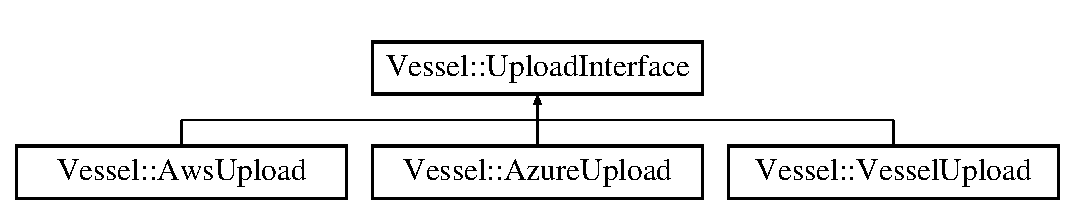
\includegraphics[height=2.000000cm]{class_vessel_1_1_upload_interface}
\end{center}
\end{figure}
\subsection*{Public Member Functions}
\begin{DoxyCompactItemize}
\item 
\mbox{\Hypertarget{class_vessel_1_1_upload_interface_a9608a8f2800d7f8a36bb30df386e4d5a}\label{class_vessel_1_1_upload_interface_a9608a8f2800d7f8a36bb30df386e4d5a}} 
virtual void {\bfseries upload\+\_\+file} (\hyperlink{class_vessel_1_1_file_1_1_file_upload}{File\+Upload} \&upload)
\item 
\mbox{\Hypertarget{class_vessel_1_1_upload_interface_ab2f7c907ca97e28c7e7478faf5135a57}\label{class_vessel_1_1_upload_interface_ab2f7c907ca97e28c7e7478faf5135a57}} 
virtual void {\bfseries resume\+\_\+uploads} ()
\item 
\mbox{\Hypertarget{class_vessel_1_1_upload_interface_a61be77a84133c6ada34c2ac20a536bdc}\label{class_vessel_1_1_upload_interface_a61be77a84133c6ada34c2ac20a536bdc}} 
virtual void {\bfseries complete\+\_\+upload} ()
\end{DoxyCompactItemize}
\subsection*{Protected Member Functions}
\begin{DoxyCompactItemize}
\item 
\mbox{\Hypertarget{class_vessel_1_1_upload_interface_ab69d8698fdeda1c88706ce0e7b96e97d}\label{class_vessel_1_1_upload_interface_ab69d8698fdeda1c88706ce0e7b96e97d}} 
std\+::shared\+\_\+ptr$<$ \hyperlink{class_vessel_1_1_networking_1_1_vessel_client}{Vessel\+Client} $>$ {\bfseries get\+\_\+vessel\+\_\+client} ()
\end{DoxyCompactItemize}


The documentation for this class was generated from the following file\+:\begin{DoxyCompactItemize}
\item 
/home/kyle/cpp/bv-\/backup/include/vessel/vessel/upload\+\_\+manager.\+hpp\end{DoxyCompactItemize}

\hypertarget{class_vessel_1_1_upload_manager}{}\section{Vessel\+:\+:Upload\+Manager Class Reference}
\label{class_vessel_1_1_upload_manager}\index{Vessel\+::\+Upload\+Manager@{Vessel\+::\+Upload\+Manager}}
\subsection*{Public Member Functions}
\begin{DoxyCompactItemize}
\item 
\mbox{\Hypertarget{class_vessel_1_1_upload_manager_a970b8771380570df1b9e806d511b89ec}\label{class_vessel_1_1_upload_manager_a970b8771380570df1b9e806d511b89ec}} 
{\bfseries Upload\+Manager} (const \hyperlink{struct_vessel_1_1_types_1_1_storage_provider}{Storage\+Provider} \&provider)
\item 
\mbox{\Hypertarget{class_vessel_1_1_upload_manager_a784c68f70fe1fc92f5a96eaecd478bb6}\label{class_vessel_1_1_upload_manager_a784c68f70fe1fc92f5a96eaecd478bb6}} 
void {\bfseries run\+\_\+uploader} ()
\end{DoxyCompactItemize}
\subsection*{Protected Member Functions}
\begin{DoxyCompactItemize}
\item 
std\+::shared\+\_\+ptr$<$ \hyperlink{class_vessel_1_1_upload_interface}{Upload\+Interface} $>$ \hyperlink{class_vessel_1_1_upload_manager_af14717ef86433c109f5429671b3ea0fd}{get\+\_\+upload\+\_\+service} (const std\+::string \&provider\+\_\+type)
\begin{DoxyCompactList}\small\item\em Returns upload service interface for a given provider type. \end{DoxyCompactList}\end{DoxyCompactItemize}


\subsection{Member Function Documentation}
\mbox{\Hypertarget{class_vessel_1_1_upload_manager_af14717ef86433c109f5429671b3ea0fd}\label{class_vessel_1_1_upload_manager_af14717ef86433c109f5429671b3ea0fd}} 
\index{Vessel\+::\+Upload\+Manager@{Vessel\+::\+Upload\+Manager}!get\+\_\+upload\+\_\+service@{get\+\_\+upload\+\_\+service}}
\index{get\+\_\+upload\+\_\+service@{get\+\_\+upload\+\_\+service}!Vessel\+::\+Upload\+Manager@{Vessel\+::\+Upload\+Manager}}
\subsubsection{\texorpdfstring{get\+\_\+upload\+\_\+service()}{get\_upload\_service()}}
{\footnotesize\ttfamily std\+::shared\+\_\+ptr$<$ \hyperlink{class_vessel_1_1_upload_interface}{Upload\+Interface} $>$ Vessel\+::\+Upload\+Manager\+::get\+\_\+upload\+\_\+service (\begin{DoxyParamCaption}\item[{const std\+::string \&}]{provider\+\_\+type }\end{DoxyParamCaption})\hspace{0.3cm}{\ttfamily [protected]}}



Returns upload service interface for a given provider type. 

\begin{DoxyReturn}{Returns}
Returns upload service interface for a given provider type 
\end{DoxyReturn}


The documentation for this class was generated from the following file\+:\begin{DoxyCompactItemize}
\item 
/home/kyle/cpp/bv-\/backup/include/vessel/vessel/upload\+\_\+manager.\+hpp\end{DoxyCompactItemize}

\hypertarget{struct_vessel_1_1_types_1_1_upload_tag_set}{}\section{Vessel\+:\+:Types\+:\+:Upload\+Tag\+Set Struct Reference}
\label{struct_vessel_1_1_types_1_1_upload_tag_set}\index{Vessel\+::\+Types\+::\+Upload\+Tag\+Set@{Vessel\+::\+Types\+::\+Upload\+Tag\+Set}}
\subsection*{Public Attributes}
\begin{DoxyCompactItemize}
\item 
\mbox{\Hypertarget{struct_vessel_1_1_types_1_1_upload_tag_set_a3fd14cdd1f64bd9e6fee9a8cc85ffab9}\label{struct_vessel_1_1_types_1_1_upload_tag_set_a3fd14cdd1f64bd9e6fee9a8cc85ffab9}} 
int {\bfseries part\+\_\+number}
\item 
\mbox{\Hypertarget{struct_vessel_1_1_types_1_1_upload_tag_set_a5409400aff1c66c0ed4f1d39d4538bbf}\label{struct_vessel_1_1_types_1_1_upload_tag_set_a5409400aff1c66c0ed4f1d39d4538bbf}} 
std\+::string {\bfseries tag}
\end{DoxyCompactItemize}


The documentation for this struct was generated from the following file\+:\begin{DoxyCompactItemize}
\item 
/home/kyle/cpp/bv-\/backup/include/vessel/types.\+hpp\end{DoxyCompactItemize}

\hypertarget{class_vessel_1_1_networking_1_1_vessel_client}{}\section{Vessel\+:\+:Networking\+:\+:Vessel\+Client Class Reference}
\label{class_vessel_1_1_networking_1_1_vessel_client}\index{Vessel\+::\+Networking\+::\+Vessel\+Client@{Vessel\+::\+Networking\+::\+Vessel\+Client}}
Inheritance diagram for Vessel\+:\+:Networking\+:\+:Vessel\+Client\+:\begin{figure}[H]
\begin{center}
\leavevmode
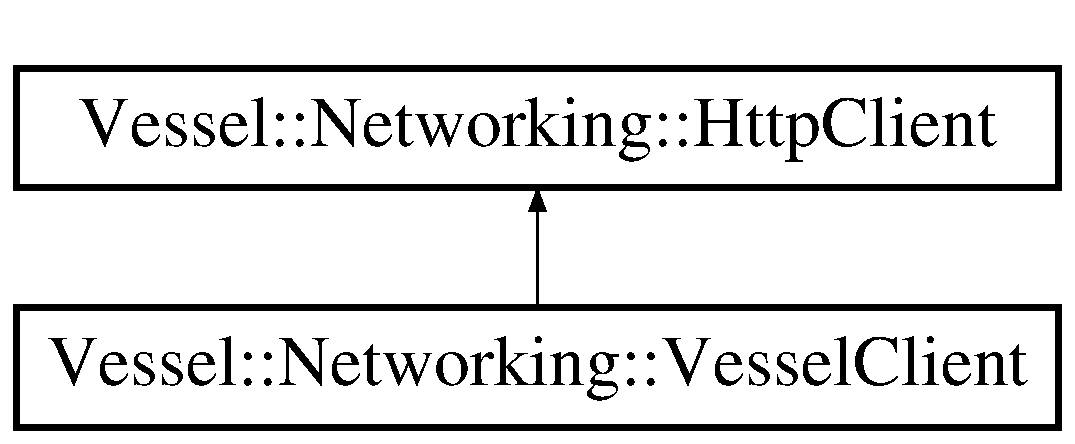
\includegraphics[height=2.000000cm]{class_vessel_1_1_networking_1_1_vessel_client}
\end{center}
\end{figure}
\subsection*{Public Member Functions}
\begin{DoxyCompactItemize}
\item 
\mbox{\Hypertarget{class_vessel_1_1_networking_1_1_vessel_client_a8ab68fa2eff83b6439e92194d2077100}\label{class_vessel_1_1_networking_1_1_vessel_client_a8ab68fa2eff83b6439e92194d2077100}} 
{\bfseries Vessel\+Client} (const std\+::string \&hostname)
\item 
std\+::string \hyperlink{class_vessel_1_1_networking_1_1_vessel_client_af024f2016833bd9887d8717e7902f1f4}{init\+\_\+upload} (const \hyperlink{class_vessel_1_1_file_1_1_backup_file}{Vessel\+::\+File\+::\+Backup\+File} \&bf)
\begin{DoxyCompactList}\small\item\em Initialize a new file upload with the Vessel R\+E\+ST A\+PI. \end{DoxyCompactList}\item 
bool \hyperlink{class_vessel_1_1_networking_1_1_vessel_client_ad24179750d17d6314c1c76b0836935b7}{upload\+\_\+file\+\_\+part} (\hyperlink{class_vessel_1_1_file_1_1_backup_file}{Vessel\+::\+File\+::\+Backup\+File} $\ast$bf, int part\+\_\+number)
\begin{DoxyCompactList}\small\item\em Sends part of a file (or the entire file) to the server with metadata. \end{DoxyCompactList}\item 
\mbox{\Hypertarget{class_vessel_1_1_networking_1_1_vessel_client_a0b2ae6947b82965aa086eed7214a6e38}\label{class_vessel_1_1_networking_1_1_vessel_client_a0b2ae6947b82965aa086eed7214a6e38}} 
void \hyperlink{class_vessel_1_1_networking_1_1_vessel_client_a0b2ae6947b82965aa086eed7214a6e38}{heartbeat} ()
\begin{DoxyCompactList}\small\item\em Sends a heartbeat payload to the Vessel A\+PI. A\+PI returns client settings and other data back to the client. \end{DoxyCompactList}\item 
bool \hyperlink{class_vessel_1_1_networking_1_1_vessel_client_ac9236da3c448454791a1c0dff1103f8a}{has\+\_\+deployment\+\_\+key} ()
\begin{DoxyCompactList}\small\item\em Returns true if the deployment\+\_\+key setting has been set. \end{DoxyCompactList}\item 
bool \hyperlink{class_vessel_1_1_networking_1_1_vessel_client_af517d80b8e5a5941ee532faae46660be}{has\+\_\+client\+\_\+token} ()
\begin{DoxyCompactList}\small\item\em Returns true if the client\+\_\+token setting has been set. \end{DoxyCompactList}\item 
\mbox{\Hypertarget{class_vessel_1_1_networking_1_1_vessel_client_a6f16e4d275f2a4e8e1671b825e708ceb}\label{class_vessel_1_1_networking_1_1_vessel_client_a6f16e4d275f2a4e8e1671b825e708ceb}} 
void \hyperlink{class_vessel_1_1_networking_1_1_vessel_client_a6f16e4d275f2a4e8e1671b825e708ceb}{install\+\_\+client} ()
\begin{DoxyCompactList}\small\item\em Installs and initializes the client application with the Vessel A\+PI using the deployment key. \end{DoxyCompactList}\item 
\hyperlink{struct_vessel_1_1_types_1_1_storage_provider}{Storage\+Provider} \hyperlink{class_vessel_1_1_networking_1_1_vessel_client_abebbf619a43e9d72ba8b6a4868b396e3}{get\+\_\+storage\+\_\+provider} ()
\begin{DoxyCompactList}\small\item\em Returns the highest priority storage provider. \end{DoxyCompactList}\item 
\mbox{\Hypertarget{class_vessel_1_1_networking_1_1_vessel_client_ae4c7ae341a369a4d310998a6a2eb76b9}\label{class_vessel_1_1_networking_1_1_vessel_client_ae4c7ae341a369a4d310998a6a2eb76b9}} 
void {\bfseries refresh\+\_\+client\+\_\+token} ()
\end{DoxyCompactItemize}
\subsection*{Additional Inherited Members}


\subsection{Member Function Documentation}
\mbox{\Hypertarget{class_vessel_1_1_networking_1_1_vessel_client_abebbf619a43e9d72ba8b6a4868b396e3}\label{class_vessel_1_1_networking_1_1_vessel_client_abebbf619a43e9d72ba8b6a4868b396e3}} 
\index{Vessel\+::\+Networking\+::\+Vessel\+Client@{Vessel\+::\+Networking\+::\+Vessel\+Client}!get\+\_\+storage\+\_\+provider@{get\+\_\+storage\+\_\+provider}}
\index{get\+\_\+storage\+\_\+provider@{get\+\_\+storage\+\_\+provider}!Vessel\+::\+Networking\+::\+Vessel\+Client@{Vessel\+::\+Networking\+::\+Vessel\+Client}}
\subsubsection{\texorpdfstring{get\+\_\+storage\+\_\+provider()}{get\_storage\_provider()}}
{\footnotesize\ttfamily \hyperlink{struct_vessel_1_1_types_1_1_storage_provider}{Storage\+Provider} Vessel\+::\+Networking\+::\+Vessel\+Client\+::get\+\_\+storage\+\_\+provider (\begin{DoxyParamCaption}{ }\end{DoxyParamCaption})}



Returns the highest priority storage provider. 

\begin{DoxyReturn}{Returns}
Returns the highest priority storage provider 
\end{DoxyReturn}
\mbox{\Hypertarget{class_vessel_1_1_networking_1_1_vessel_client_af517d80b8e5a5941ee532faae46660be}\label{class_vessel_1_1_networking_1_1_vessel_client_af517d80b8e5a5941ee532faae46660be}} 
\index{Vessel\+::\+Networking\+::\+Vessel\+Client@{Vessel\+::\+Networking\+::\+Vessel\+Client}!has\+\_\+client\+\_\+token@{has\+\_\+client\+\_\+token}}
\index{has\+\_\+client\+\_\+token@{has\+\_\+client\+\_\+token}!Vessel\+::\+Networking\+::\+Vessel\+Client@{Vessel\+::\+Networking\+::\+Vessel\+Client}}
\subsubsection{\texorpdfstring{has\+\_\+client\+\_\+token()}{has\_client\_token()}}
{\footnotesize\ttfamily bool Vessel\+::\+Networking\+::\+Vessel\+Client\+::has\+\_\+client\+\_\+token (\begin{DoxyParamCaption}{ }\end{DoxyParamCaption})}



Returns true if the client\+\_\+token setting has been set. 

\begin{DoxyReturn}{Returns}
Returns true if the client\+\_\+token setting has been set 
\end{DoxyReturn}
\mbox{\Hypertarget{class_vessel_1_1_networking_1_1_vessel_client_ac9236da3c448454791a1c0dff1103f8a}\label{class_vessel_1_1_networking_1_1_vessel_client_ac9236da3c448454791a1c0dff1103f8a}} 
\index{Vessel\+::\+Networking\+::\+Vessel\+Client@{Vessel\+::\+Networking\+::\+Vessel\+Client}!has\+\_\+deployment\+\_\+key@{has\+\_\+deployment\+\_\+key}}
\index{has\+\_\+deployment\+\_\+key@{has\+\_\+deployment\+\_\+key}!Vessel\+::\+Networking\+::\+Vessel\+Client@{Vessel\+::\+Networking\+::\+Vessel\+Client}}
\subsubsection{\texorpdfstring{has\+\_\+deployment\+\_\+key()}{has\_deployment\_key()}}
{\footnotesize\ttfamily bool Vessel\+::\+Networking\+::\+Vessel\+Client\+::has\+\_\+deployment\+\_\+key (\begin{DoxyParamCaption}{ }\end{DoxyParamCaption})}



Returns true if the deployment\+\_\+key setting has been set. 

\begin{DoxyReturn}{Returns}
Returns true if the deployment\+\_\+key setting has been set 
\end{DoxyReturn}
\mbox{\Hypertarget{class_vessel_1_1_networking_1_1_vessel_client_af024f2016833bd9887d8717e7902f1f4}\label{class_vessel_1_1_networking_1_1_vessel_client_af024f2016833bd9887d8717e7902f1f4}} 
\index{Vessel\+::\+Networking\+::\+Vessel\+Client@{Vessel\+::\+Networking\+::\+Vessel\+Client}!init\+\_\+upload@{init\+\_\+upload}}
\index{init\+\_\+upload@{init\+\_\+upload}!Vessel\+::\+Networking\+::\+Vessel\+Client@{Vessel\+::\+Networking\+::\+Vessel\+Client}}
\subsubsection{\texorpdfstring{init\+\_\+upload()}{init\_upload()}}
{\footnotesize\ttfamily std\+::string Vessel\+::\+Networking\+::\+Vessel\+Client\+::init\+\_\+upload (\begin{DoxyParamCaption}\item[{const \hyperlink{class_vessel_1_1_file_1_1_backup_file}{Vessel\+::\+File\+::\+Backup\+File} \&}]{bf }\end{DoxyParamCaption})}



Initialize a new file upload with the Vessel R\+E\+ST A\+PI. 

\begin{DoxyReturn}{Returns}
Returns the Vessel file id from the A\+PI 
\end{DoxyReturn}
\mbox{\Hypertarget{class_vessel_1_1_networking_1_1_vessel_client_ad24179750d17d6314c1c76b0836935b7}\label{class_vessel_1_1_networking_1_1_vessel_client_ad24179750d17d6314c1c76b0836935b7}} 
\index{Vessel\+::\+Networking\+::\+Vessel\+Client@{Vessel\+::\+Networking\+::\+Vessel\+Client}!upload\+\_\+file\+\_\+part@{upload\+\_\+file\+\_\+part}}
\index{upload\+\_\+file\+\_\+part@{upload\+\_\+file\+\_\+part}!Vessel\+::\+Networking\+::\+Vessel\+Client@{Vessel\+::\+Networking\+::\+Vessel\+Client}}
\subsubsection{\texorpdfstring{upload\+\_\+file\+\_\+part()}{upload\_file\_part()}}
{\footnotesize\ttfamily Vessel\+::\+Networking\+::\+Vessel\+Client\+::upload\+\_\+file\+\_\+part (\begin{DoxyParamCaption}\item[{\hyperlink{class_vessel_1_1_file_1_1_backup_file}{Vessel\+::\+File\+::\+Backup\+File} $\ast$}]{bf,  }\item[{int}]{part\+\_\+number }\end{DoxyParamCaption})}



Sends part of a file (or the entire file) to the server with metadata. 


\begin{DoxyParams}{Parameters}
{\em bf} & Backup\+File object \\
\hline
{\em part\+\_\+number} & The part or chunk number of the file content being uploaded \\
\hline
\end{DoxyParams}
\begin{DoxyReturn}{Returns}
Returns true if successful, false if there were errors 
\end{DoxyReturn}


The documentation for this class was generated from the following file\+:\begin{DoxyCompactItemize}
\item 
/home/kyle/cpp/bv-\/backup/include/vessel/vessel/vessel\+\_\+client.\+hpp\end{DoxyCompactItemize}

\hypertarget{class_vessel_1_1_exception_1_1_vessel_exception}{}\section{Vessel\+:\+:Exception\+:\+:Vessel\+Exception Class Reference}
\label{class_vessel_1_1_exception_1_1_vessel_exception}\index{Vessel\+::\+Exception\+::\+Vessel\+Exception@{Vessel\+::\+Exception\+::\+Vessel\+Exception}}
Inheritance diagram for Vessel\+:\+:Exception\+:\+:Vessel\+Exception\+:\begin{figure}[H]
\begin{center}
\leavevmode
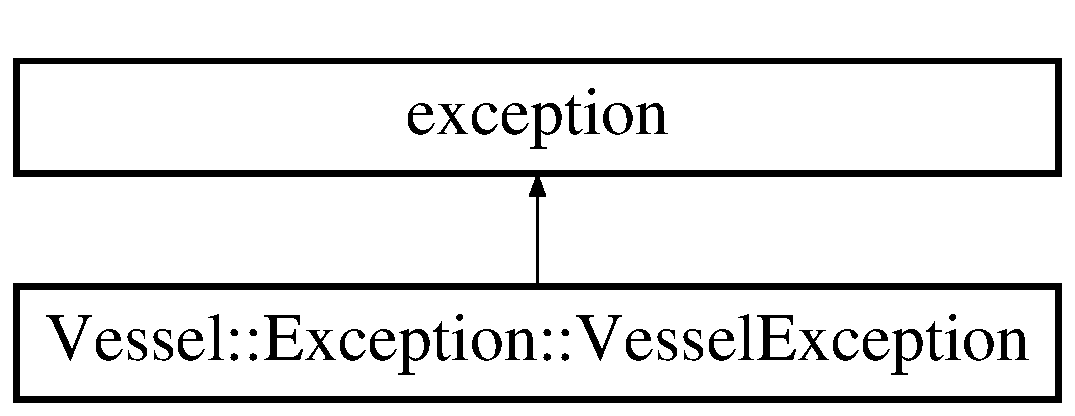
\includegraphics[height=2.000000cm]{class_vessel_1_1_exception_1_1_vessel_exception}
\end{center}
\end{figure}
\subsection*{Public Types}
\begin{DoxyCompactItemize}
\item 
\mbox{\Hypertarget{class_vessel_1_1_exception_1_1_vessel_exception_a5457467e292ffcdd46a30131315c6c0c}\label{class_vessel_1_1_exception_1_1_vessel_exception_a5457467e292ffcdd46a30131315c6c0c}} 
enum {\bfseries Error\+Code} \{ {\bfseries No\+Error} = 0, 
{\bfseries Not\+Installed}, 
{\bfseries Provider\+Error}, 
{\bfseries Bad\+Upload}
 \}
\end{DoxyCompactItemize}
\subsection*{Public Member Functions}
\begin{DoxyCompactItemize}
\item 
\mbox{\Hypertarget{class_vessel_1_1_exception_1_1_vessel_exception_afa4dbc0e78bd83c75a7628ad082a1b64}\label{class_vessel_1_1_exception_1_1_vessel_exception_afa4dbc0e78bd83c75a7628ad082a1b64}} 
{\bfseries Vessel\+Exception} (Error\+Code e, const std\+::string \&msg)
\item 
\mbox{\Hypertarget{class_vessel_1_1_exception_1_1_vessel_exception_a794da64632d4c4898bea4d2ab7cb4944}\label{class_vessel_1_1_exception_1_1_vessel_exception_a794da64632d4c4898bea4d2ab7cb4944}} 
Error\+Code {\bfseries get\+\_\+code} ()
\item 
\mbox{\Hypertarget{class_vessel_1_1_exception_1_1_vessel_exception_acb457998178a3e47c7798eae0fc2e92a}\label{class_vessel_1_1_exception_1_1_vessel_exception_acb457998178a3e47c7798eae0fc2e92a}} 
virtual const char $\ast$ {\bfseries what} () const noexcept override
\end{DoxyCompactItemize}


The documentation for this class was generated from the following file\+:\begin{DoxyCompactItemize}
\item 
/home/kyle/cpp/bv-\/backup/include/vessel/vessel/vessel\+\_\+exception.\+hpp\end{DoxyCompactItemize}

\hypertarget{class_vessel_1_1_vessel_upload}{}\section{Vessel\+:\+:Vessel\+Upload Class Reference}
\label{class_vessel_1_1_vessel_upload}\index{Vessel\+::\+Vessel\+Upload@{Vessel\+::\+Vessel\+Upload}}
Inheritance diagram for Vessel\+:\+:Vessel\+Upload\+:\begin{figure}[H]
\begin{center}
\leavevmode
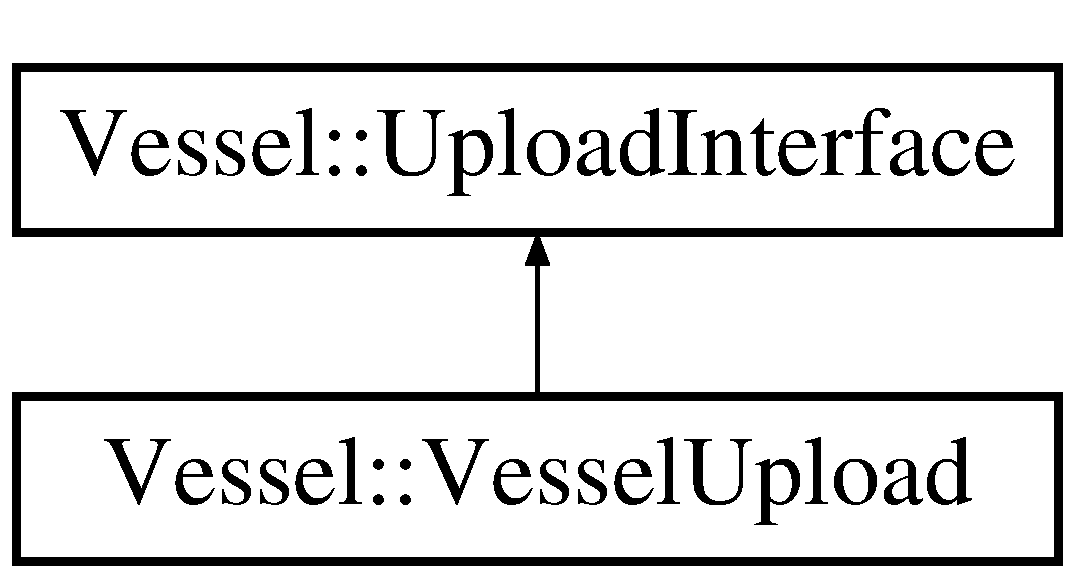
\includegraphics[height=2.000000cm]{class_vessel_1_1_vessel_upload}
\end{center}
\end{figure}
\subsection*{Public Member Functions}
\begin{DoxyCompactItemize}
\item 
\mbox{\Hypertarget{class_vessel_1_1_vessel_upload_af1f2f3fd9ca8d201139b599797fde9c5}\label{class_vessel_1_1_vessel_upload_af1f2f3fd9ca8d201139b599797fde9c5}} 
virtual void {\bfseries upload\+\_\+file} ()
\item 
\mbox{\Hypertarget{class_vessel_1_1_vessel_upload_aa32f2e15f511307c9797287a1770e7a0}\label{class_vessel_1_1_vessel_upload_aa32f2e15f511307c9797287a1770e7a0}} 
virtual void {\bfseries resume\+\_\+uploads} ()
\item 
\mbox{\Hypertarget{class_vessel_1_1_vessel_upload_a0a4b77ac363e86f66138db578ca9ca38}\label{class_vessel_1_1_vessel_upload_a0a4b77ac363e86f66138db578ca9ca38}} 
virtual void {\bfseries complete\+\_\+upload} ()
\end{DoxyCompactItemize}
\subsection*{Additional Inherited Members}


The documentation for this class was generated from the following file\+:\begin{DoxyCompactItemize}
\item 
/home/kyle/cpp/bv-\/backup/include/vessel/vessel/upload\+\_\+manager.\+hpp\end{DoxyCompactItemize}

%--- End generated contents ---

% Index
\backmatter
\newpage
\phantomsection
\clearemptydoublepage
\addcontentsline{toc}{chapter}{Index}
\printindex

\end{document}
